% Options for packages loaded elsewhere
\PassOptionsToPackage{unicode}{hyperref}
\PassOptionsToPackage{hyphens}{url}
%
\documentclass[
  man, donotrepeattitle,floatsintext]{apa6}
\usepackage{amsmath,amssymb}
\usepackage{lmodern}
\usepackage{iftex}
\ifPDFTeX
  \usepackage[T1]{fontenc}
  \usepackage[utf8]{inputenc}
  \usepackage{textcomp} % provide euro and other symbols
\else % if luatex or xetex
  \usepackage{unicode-math}
  \defaultfontfeatures{Scale=MatchLowercase}
  \defaultfontfeatures[\rmfamily]{Ligatures=TeX,Scale=1}
\fi
% Use upquote if available, for straight quotes in verbatim environments
\IfFileExists{upquote.sty}{\usepackage{upquote}}{}
\IfFileExists{microtype.sty}{% use microtype if available
  \usepackage[]{microtype}
  \UseMicrotypeSet[protrusion]{basicmath} % disable protrusion for tt fonts
}{}
\makeatletter
\@ifundefined{KOMAClassName}{% if non-KOMA class
  \IfFileExists{parskip.sty}{%
    \usepackage{parskip}
  }{% else
    \setlength{\parindent}{0pt}
    \setlength{\parskip}{6pt plus 2pt minus 1pt}}
}{% if KOMA class
  \KOMAoptions{parskip=half}}
\makeatother
\usepackage{xcolor}
\usepackage{graphicx}
\makeatletter
\def\maxwidth{\ifdim\Gin@nat@width>\linewidth\linewidth\else\Gin@nat@width\fi}
\def\maxheight{\ifdim\Gin@nat@height>\textheight\textheight\else\Gin@nat@height\fi}
\makeatother
% Scale images if necessary, so that they will not overflow the page
% margins by default, and it is still possible to overwrite the defaults
% using explicit options in \includegraphics[width, height, ...]{}
\setkeys{Gin}{width=\maxwidth,height=\maxheight,keepaspectratio}
% Set default figure placement to htbp
\makeatletter
\def\fps@figure{htbp}
\makeatother
\setlength{\emergencystretch}{3em} % prevent overfull lines
\providecommand{\tightlist}{%
  \setlength{\itemsep}{0pt}\setlength{\parskip}{0pt}}
\setcounter{secnumdepth}{-\maxdimen} % remove section numbering
% Make \paragraph and \subparagraph free-standing
\ifx\paragraph\undefined\else
  \let\oldparagraph\paragraph
  \renewcommand{\paragraph}[1]{\oldparagraph{#1}\mbox{}}
\fi
\ifx\subparagraph\undefined\else
  \let\oldsubparagraph\subparagraph
  \renewcommand{\subparagraph}[1]{\oldsubparagraph{#1}\mbox{}}
\fi
\newlength{\cslhangindent}
\setlength{\cslhangindent}{1.5em}
\newlength{\csllabelwidth}
\setlength{\csllabelwidth}{3em}
\newlength{\cslentryspacingunit} % times entry-spacing
\setlength{\cslentryspacingunit}{\parskip}
\newenvironment{CSLReferences}[2] % #1 hanging-ident, #2 entry spacing
 {% don't indent paragraphs
  \setlength{\parindent}{0pt}
  % turn on hanging indent if param 1 is 1
  \ifodd #1
  \let\oldpar\par
  \def\par{\hangindent=\cslhangindent\oldpar}
  \fi
  % set entry spacing
  \setlength{\parskip}{#2\cslentryspacingunit}
 }%
 {}
\usepackage{calc}
\newcommand{\CSLBlock}[1]{#1\hfill\break}
\newcommand{\CSLLeftMargin}[1]{\parbox[t]{\csllabelwidth}{#1}}
\newcommand{\CSLRightInline}[1]{\parbox[t]{\linewidth - \csllabelwidth}{#1}\break}
\newcommand{\CSLIndent}[1]{\hspace{\cslhangindent}#1}
\ifLuaTeX
\usepackage[bidi=basic]{babel}
\else
\usepackage[bidi=default]{babel}
\fi
\babelprovide[main,import]{english}
% get rid of language-specific shorthands (see #6817):
\let\LanguageShortHands\languageshorthands
\def\languageshorthands#1{}
% Manuscript styling
\usepackage{upgreek}
\captionsetup{font=singlespacing,justification=justified}

% Table formatting
\usepackage{longtable}
\usepackage{lscape}
% \usepackage[counterclockwise]{rotating}   % Landscape page setup for large tables
\usepackage{multirow}		% Table styling
\usepackage{tabularx}		% Control Column width
\usepackage[flushleft]{threeparttable}	% Allows for three part tables with a specified notes section
\usepackage{threeparttablex}            % Lets threeparttable work with longtable

% Create new environments so endfloat can handle them
% \newenvironment{ltable}
%   {\begin{landscape}\centering\begin{threeparttable}}
%   {\end{threeparttable}\end{landscape}}
\newenvironment{lltable}{\begin{landscape}\centering\begin{ThreePartTable}}{\end{ThreePartTable}\end{landscape}}

% Enables adjusting longtable caption width to table width
% Solution found at http://golatex.de/longtable-mit-caption-so-breit-wie-die-tabelle-t15767.html
\makeatletter
\newcommand\LastLTentrywidth{1em}
\newlength\longtablewidth
\setlength{\longtablewidth}{1in}
\newcommand{\getlongtablewidth}{\begingroup \ifcsname LT@\roman{LT@tables}\endcsname \global\longtablewidth=0pt \renewcommand{\LT@entry}[2]{\global\advance\longtablewidth by ##2\relax\gdef\LastLTentrywidth{##2}}\@nameuse{LT@\roman{LT@tables}} \fi \endgroup}

% \setlength{\parindent}{0.5in}
% \setlength{\parskip}{0pt plus 0pt minus 0pt}

% Overwrite redefinition of paragraph and subparagraph by the default LaTeX template
% See https://github.com/crsh/papaja/issues/292
\makeatletter
\renewcommand{\paragraph}{\@startsection{paragraph}{4}{\parindent}%
  {0\baselineskip \@plus 0.2ex \@minus 0.2ex}%
  {-1em}%
  {\normalfont\normalsize\bfseries\itshape\typesectitle}}

\renewcommand{\subparagraph}[1]{\@startsection{subparagraph}{5}{1em}%
  {0\baselineskip \@plus 0.2ex \@minus 0.2ex}%
  {-\z@\relax}%
  {\normalfont\normalsize\itshape\hspace{\parindent}{#1}\textit{\addperi}}{\relax}}
\makeatother

% \usepackage{etoolbox}
\makeatletter
\patchcmd{\HyOrg@maketitle}
  {\section{\normalfont\normalsize\abstractname}}
  {\section*{\normalfont\normalsize\abstractname}}
  {}{\typeout{Failed to patch abstract.}}
\patchcmd{\HyOrg@maketitle}
  {\section{\protect\normalfont{\@title}}}
  {\section*{\protect\normalfont{\@title}}}
  {}{\typeout{Failed to patch title.}}
\makeatother

\usepackage{xpatch}
\makeatletter
\xapptocmd\appendix
  {\xapptocmd\section
    {\addcontentsline{toc}{section}{\appendixname\ifoneappendix\else~\theappendix\fi\\: #1}}
    {}{\InnerPatchFailed}%
  }
{}{\PatchFailed}
\keywords{tool use; technical intelligence; parrots; digital video platforms; phylogenetic modelling}
\usepackage{lineno}

\linenumbers
\usepackage{csquotes}
\usepackage{array}
\usepackage{caption}
\usepackage{graphicx}
\usepackage{siunitx}
\usepackage[normalem]{ulem}
\usepackage{colortbl}
\usepackage{multirow}
\usepackage{hhline}
\usepackage{calc}
\usepackage{tabularx}
\usepackage{threeparttable}
\usepackage{wrapfig}
\usepackage{adjustbox}
\usepackage{hyperref}
\usepackage{setspace}
\raggedbottom
\AtBeginEnvironment{tabular}{\singlespacing}
\AtBeginEnvironment{lltable}{\singlespacing}
\AtBeginEnvironment{tablenotes}{\doublespacing}
\captionsetup[table]{font={stretch=1,small}}
\captionsetup[figure]{font={stretch=1,small}}
\nolinenumbers
\note{\raggedright † These authors contributed equally to this work \par ‡ These authors contributed equally to this work \par * Correspondence concerning this article should be addressed to Scott Claessens, Level 2, Building 302, 23 Symonds Street, Auckland, New Zealand. \text{E-mail:} \href{scott.claessens@gmail.com}{\nolinkurl{scott.claessens@gmail.com}} \par This working paper has not yet been peer-reviewed.}
\ifLuaTeX
  \usepackage{selnolig}  % disable illegal ligatures
\fi
\IfFileExists{bookmark.sty}{\usepackage{bookmark}}{\usepackage{hyperref}}
\IfFileExists{xurl.sty}{\usepackage{xurl}}{} % add URL line breaks if available
\urlstyle{same} % disable monospaced font for URLs
\hypersetup{
  pdftitle={Evidence of self-care tooling on digital video platforms and phylogenetic modelling reveal parrot tool use is not rare},
  pdfauthor={Amalia P. M. Bastos†,1,2, Scott Claessens*†,2, Ximena J. Nelson3, David Welch4, Quentin D. Atkinson‡,2, \& Alex H. Taylor‡,2,3,5,6},
  pdflang={en-EN},
  pdfkeywords={tool use; technical intelligence; parrots; digital video platforms; phylogenetic modelling},
  hidelinks,
  pdfcreator={LaTeX via pandoc}}

\title{Evidence of self-care tooling on digital video platforms and phylogenetic modelling reveal parrot tool use is not rare}
\author{Amalia P. M. Bastos\textsuperscript{†,1,2}, Scott Claessens\textsuperscript{*†,2}, Ximena J. Nelson\textsuperscript{3}, David Welch\textsuperscript{4}, Quentin D. Atkinson\textsuperscript{‡,2}, \& Alex H. Taylor\textsuperscript{‡,2,3,5,6}}
\date{}


\shorttitle{Parrot tool use}

\affiliation{\vspace{0.5cm}\textsuperscript{1} \footnotesize Department of Psychological \& Brain Sciences, Johns Hopkins University, Baltimore, MD, United States\\\textsuperscript{2} \footnotesize School of Psychology, University of Auckland, Auckland, New Zealand\\\textsuperscript{3} \footnotesize School of Biological Sciences, University of Canterbury, Christchurch, New Zealand\\\textsuperscript{4} \footnotesize School of Computer Science, University of Auckland, Auckland, New Zealand\\\textsuperscript{5} \footnotesize ICREA, Pg. Lluís Companys 23, Barcelona, Spain\\\textsuperscript{6} \footnotesize Institute of Neuroscience, Universitat Autònoma de Barcelona, Barcelona, Spain}

\abstract{%
Putatively rare behaviours, such as tool use, are challenging to study because absence of evidence can arise either from a species' inability to produce the behaviour or from insufficient research effort. Here, we tackle this challenge by combining data from digital platforms and phylogenetic modelling to estimate actual rates of tool use in parrots. Videos on a social media platform revealed novel instances of self-care tooling in 17 parrot species, more than doubling the confirmed number of tool-using parrot species from 11 (3\%) to 28 (7\%). Phylogenetic modelling ranked additional species that are most likely to be unobserved tool users, suggesting that between 11\% and 17\% of extant parrot species may be capable of tool use. These discoveries have implications for inferences about the evolutionary drivers and origins of tool use in parrots, revealing associations with relative brain size and feeding generalism and indicating several genera where tool use was likely an ancestral trait. Overall, our findings challenge the assumption that current sampling effort captures the full distribution of putatively rare animal behaviours. Combining our sampling and analysis methods offers a fruitful approach for investigating the distribution, drivers, and origins of other rare behaviours.
}



\begin{document}
\maketitle

\newpage
\linenumbers

\hypertarget{introduction}{%
\section{Introduction}\label{introduction}}

Our understanding of the evolution of animal behaviour is built on the
assumption that we have access to sufficient data\textsuperscript{1--3}. However, this is not always the case. Data on behaviours that are
rare, fleeting, or otherwise difficult to observe are likely to be patchy and
incomplete\textsuperscript{4,5}. Among species for which such behaviours
have not been observed, it can be difficult to differentiate between cases in
which the species is truly incapable of producing the behaviour and cases in
which the species is capable of producing the behaviour but the behaviour has
not yet been observed. Such a distinction can be critical for drawing
conclusions about the rarity and evolution of the behaviour in question.

Comparative work on the evolution of tool use is a paradigmatic example of this
issue. The initial discoveries of tool use in chimpanzees\textsuperscript{6},
birds\textsuperscript{7}, dolphins\textsuperscript{8}, and octopuses\textsuperscript{9} occurred
decades after significant advances on other more easily measurable aspects of
their biology. Since then, scholars have proposed a clear operational
definition of tool use applicable to all species --- the manipulation of an
unattached object as an extension of the animal's body to achieve a
goal\textsuperscript{10} --- and have used the distribution of species meeting this
definition to make various claims about the evolutionary drivers of tool use
behaviours. For example, based on the observation that bird species with
reported tool use tend to have larger brains, researchers have identified
higher relative brain size as a likely precondition for tool using
capabilities\textsuperscript{11--14}. These
researchers argue that larger brains are better able to integrate visual and
somatosensory information when innovating novel behaviours, such as tool use,
in changing environments\textsuperscript{15,16} (but see ref\textsuperscript{17}).
Similarly, researchers have used existing reports of tool use in birds to debate
the roles of generalist versus specialist feeding strategies in driving the
evolution of tool use, with some arguing that feeding generalists require
technical innovations to expand their dietary niche\textsuperscript{15,18,19} and others arguing that feeding
specialists require technical innovations for extractive foraging of specific
foods\textsuperscript{20,21}.

However, before we can make claims of this kind, we need to know whether current
research effort in the literature is sufficient for robust conclusions to be
drawn about the evolution of tool use. In fact, evidence suggests that research
effort is often systematically biased towards particular taxonomic groups, parts
of the world that are easy to access, and species with life history traits that
make them easier to study, such as larger distribution ranges and population
sizes\textsuperscript{22}. This is a crucial limitation because insufficient
observation may lead researchers to miss true instances of tool behaviours and
thus draw premature conclusions about the evolutionary drivers and origins of
tool use. Researchers are keenly aware of this problem and have attempted to
deal with it in different ways, such as controlling for the number of scientific
papers published on different species. But previous work has not yet attempted
to quantify and explicitly model the relationship between actual tool-using
behaviour and what is reported in the scientific literature. If more tool-using
species exist than previously thought, this could have important implications
for theories of the evolutionary drivers and origins of tool use and for our
understanding of how rare this behaviour actually is.

One potentially powerful method for quantifying actual rates of rare animal
behaviours is by collating evidence of the behaviours from digital video
platforms\textsuperscript{23}. With millions of videos posted every day, digital
platforms like YouTube offer a valuable source of data on animal behaviour.
Digital video platforms have already been successfully used to uncover a variety
of rare animal behaviours, including interspecies play in dogs\textsuperscript{23},
novel problem-solving behaviours in horses\textsuperscript{24}, and death-related
behaviours in Asian elephants\textsuperscript{25}. By casting the net wider than the
scientific literature, digital video platforms can provide an indication of the
tool-using species that the literature might be missing.

Even after collating evidence from digital video platforms, some tool-users
could \emph{still} remain unobserved. One principled framework for identifying these
unobserved species is to specify a causal model of the process that generates
the observed data. We propose one such causal model in Figure
\ref{fig:plotDAG}. In this model, we assume that the presence of tool use in
the scientific literature (or on digital video platforms) is caused by both
unobserved tool use capabilities and the number of published studies (or the
number of videos) for any given species. Tool users are more likely to be
observed if they are well studied, but understudied tool users may go
undetected. Furthermore, based on existing theories of the evolution of tool use\textsuperscript{12--16,18--21}, we propose
that the unobserved tool use capabilities are additionally caused by relative
brain size, feeding strategy, and shared phylogenetic ancestry. Expressing this
causal model as a statistical model can suggest further species which are likely
to be unobserved tool-users and, simultaneously, test existing theories of the
evolutionary drivers of tool use without incorrectly assuming that absence of
evidence is evidence of absence.












\begin{figure}
\centering
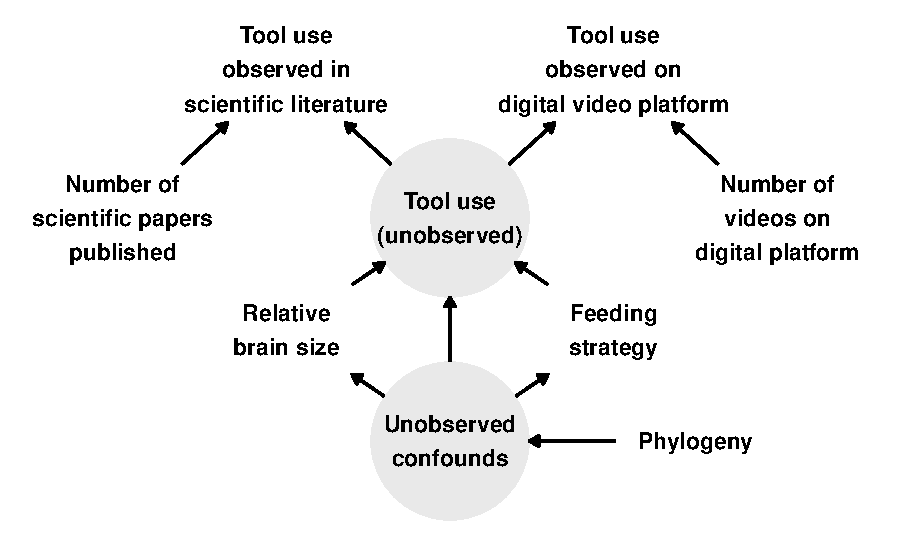
\includegraphics{manuscript_files/figure-latex/plotDAG-1.pdf}
\caption{\label{fig:plotDAG}\emph{Causal model of observed tool use.} Directed acyclic graph
of the causal relationships between observed tool use and other variables.
Available scientific data on tool use is caused both by unobserved tool use
presence and scientific research effort (i.e., number of publications).
Available video data on tool use is caused both by unobserved tool use
presence and video research effort (i.e., number of videos). According to
theory, unobserved tool use presence should be caused by relative brain size
(encephalisation quotient) and feeding strategy (generalist vs.~specialist).
These variables all share unobserved confounds generated by shared phylogenetic
history. Grey circles indicate unobserved variables.}
\end{figure}

Here, we apply these approaches to tool use in the parrot order. We focus on
tool use in parrots for a number of reasons. First, the scientific literature
suggests that only a small proportion of extant parrot species (11 out of 398;
3\%) use tools\textsuperscript{12,26--38}. Parrot tool
use thus provides an ideal test case for examining how robust sampling is in the
scientific literature. Second, parrots are popular as pets. Over 70\% of all
extant parrot species are bred in the aviculture industry and kept as pets
worldwide\textsuperscript{39--45}, enabling us to leverage the power of digital video platforms to
search for evidence of tool use\textsuperscript{23}. Third, detailed data on relative
brain sizes\textsuperscript{46--51}, feeding strategies\textsuperscript{52}, and shared ancestry\textsuperscript{53} exist for parrots, allowing us to fit the statistical model implied
by Figure \ref{fig:plotDAG} to the entire parrot order.

We first present the results from our video survey, in which we collated videos
of tool use in parrots from a digital video platform. This survey reveals that a
number of parrots not previously known to use tools are capable of self-care
tooling. We then map these previously unidentified tool-using species onto the
phylogeny of the parrot order and use a phylogenetic survival cure model to
(\emph{i}) rank further parrot species that are likely unobserved tool users and
(\emph{ii}) re-examine key hypotheses regarding the evolutionary drivers and origins
of tool use in parrots.

\hypertarget{results}{%
\section{Results}\label{results}}

\hypertarget{digital-video-platform-reveals-self-care-tool-use-in-additional-parrot-species}{%
\subsection{Digital video platform reveals self-care tool use in additional parrot species}\label{digital-video-platform-reveals-self-care-tool-use-in-additional-parrot-species}}

We surveyed the digital media platform YouTube for video evidence of tool use in
parrots (see Methods for detailed search criteria). In our search, we used the
standard criteria for identifying tool use in the literature, defining ``true''
tool use behaviour as the manipulation of an unattached object as an extension
of the animal's body to achieve a goal\textsuperscript{10}, while ``borderline'' tool
use involved the use of an object that was still attached to a substrate\textsuperscript{54}.

In total, we found 116 videos of
104 individuals from
25
parrot species performing behaviours that met the definition of either true tool
use (100 videos of
89
individuals from
22
species) or borderline tool use (16 videos of
16
individuals from
7
species). All videos featured pet parrots in captive settings performing
self-care tool use, specifically self-scratching. In
68 of these
videos, owners did not appear to interact with the subjects. In
43 videos,
there was potential human interaction, either from the owners being in close physical
contact with the bird (e.g., bird perching on hand), talking to the bird, or
handing it the tool (which occurred in only two videos). We could not establish
the degree of human interaction in the remaining
5
videos, as sound had been removed or was substituted by music. None of the
videos featured owners directly rewarding tool use behaviours with food. All
borderline tool use cases were excluded from further analyses.

Of the 22
parrot species performing true tool use for self-care,
13
were represented in our video survey by two or more individuals over multiple
independent observations. True tool use always involved the subject using an
object for self-scratching (95
videos involved scratching the head and/or neck). The most common tool (53
videos) was a moulted feather. Human-made objects (e.g., pens, spoons, pieces of
wood, cardboard) were also common. In 66
videos, parrots manipulated the tool while keeping their body still, rather than
holding the tool still and moving towards it.

According to YouTube video descriptions and owner comments,
45
of the individuals performing true tool use for self-care were males and
18
were females. No sex information was provided for the remaining
26
individuals. As owners provided no information on whether sex had been
established through genetic testing, and sexual dimorphism in parrots is
rare\textsuperscript{55,56}, we could not typically ascertain if descriptions
were accurate. It is unclear if the disproportionately large number of males in
the sample is a consequence of owners more readily assuming their parrots are
male when they have not been genetically tested, owners being more likely to own
or film male parrots, or male parrots exhibiting more self-scratching behaviours
than female parrots.

Figure \ref{fig:plotPhylo1} maps the findings from the video survey onto a
maximum clade credibility phylogeny for the parrot order, plotted alongside
species previously identified in the scientific literature. Before the video
survey, 11 parrot species (3\%) had been identified as tool users in the
scientific literature. Across our video survey, we observed true tool use for self-care in
22
species, 5 of which overlapped with the scientific literature and
17
of which were novel species. All of the species identified in the video survey
were cockatoos (\emph{Cacatuidae}), Old World parrots (\emph{Psittacinae}), or neotropical
parrots (\emph{Arinae}). The most common species in our survey, accounting for
41 videos from
37
individuals, was the green-cheeked conure (\emph{Pyrrhura molinae}). In accordance
with the scientific literature, the video survey found no evidence of tool use
in any species of Psittaculidae, despite this family containing some of the most
commonly kept pet species, including lovebirds, lorikeets, and Asian parakeet
species. Combining both the video survey and the scientific literature, we can
thus identify 28 total parrot species (7\%) capable of true tool use as defined
by ref\textsuperscript{10}, compared to the 11 previously reported.














\begin{figure}
\centering
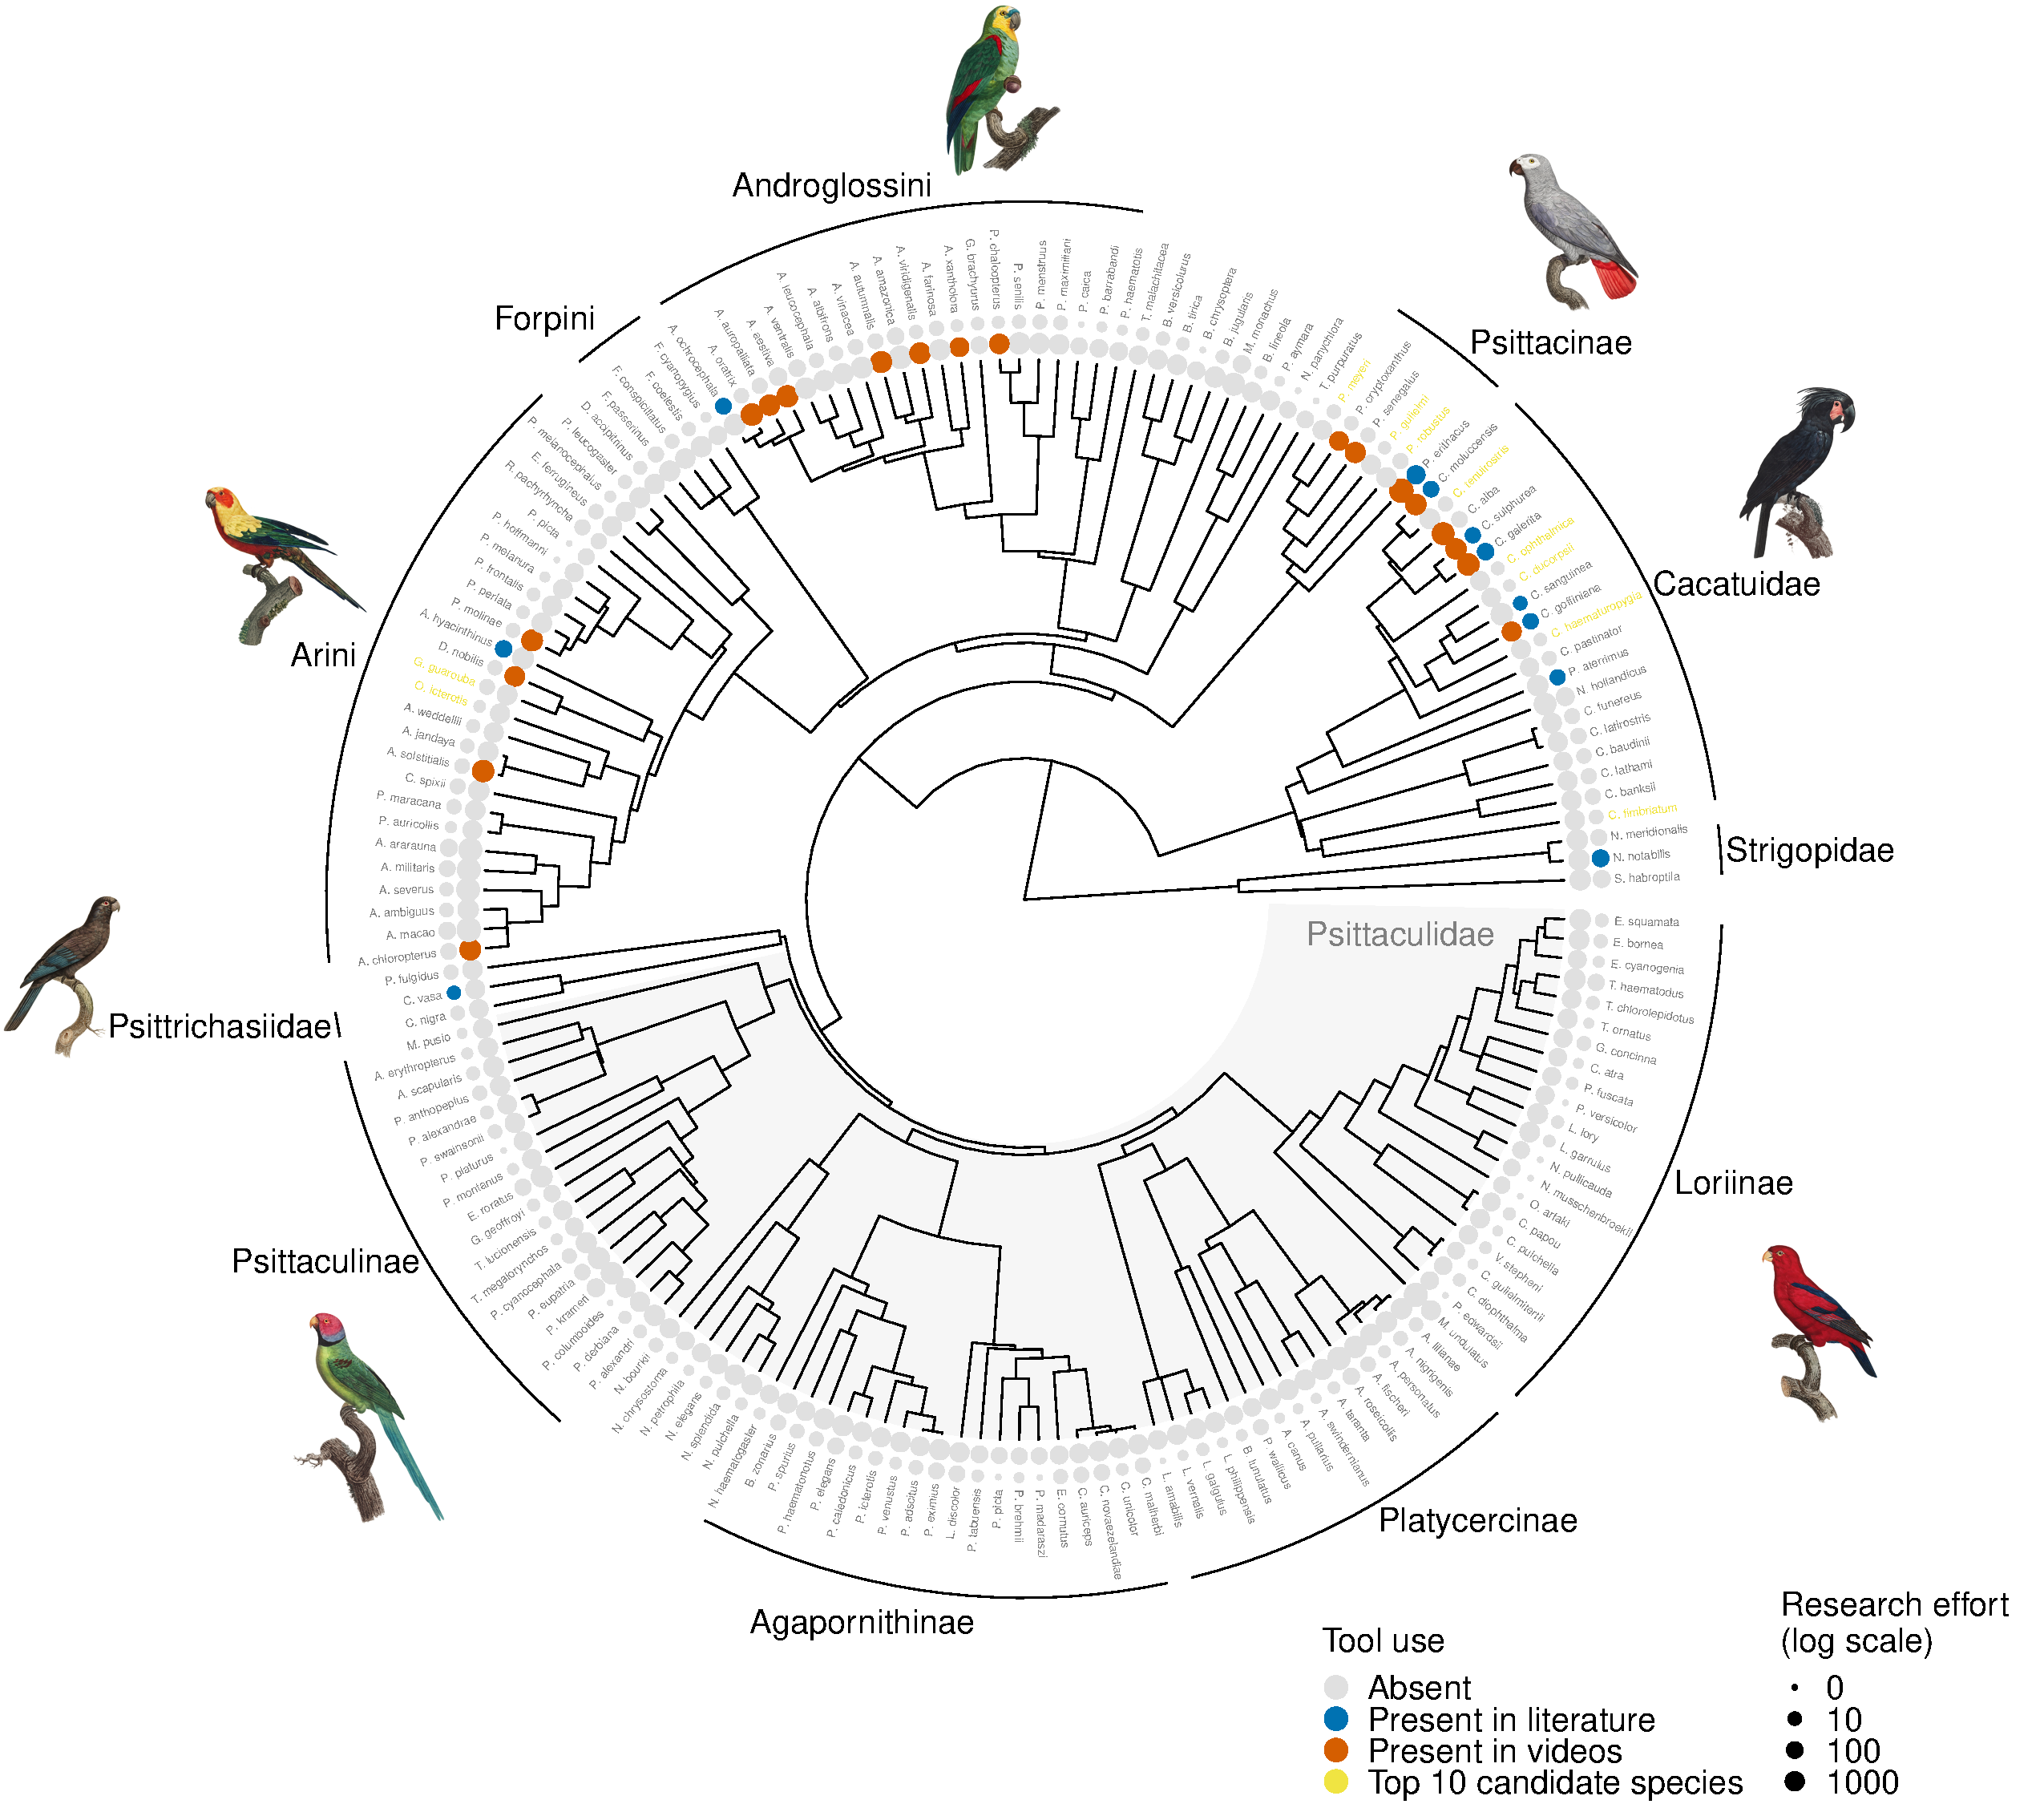
\includegraphics{manuscript_files/figure-latex/plotPhylo1-1.pdf}
\caption{\label{fig:plotPhylo1}\emph{Results of video survey and phylogenetic survival cure
modelling mapped onto a maximum clade credibility phylogeny of the parrot order.}
Orange points in the inner ring indicate species observed in the video survey,
with point size scaled by the number of videos for each species (note that three
species observed only in the video survey are not present in the phylogeny due
to a lack of genomic data: \emph{Psittacara erythrogenys}, \emph{Psittacus timneh}, and
\emph{Aratinga nenday}). Blue points in the outer ring indicate species observed in
the scientific literature, with point size scaled by the number of papers
published on each species. Yellow species names indicate the top ten most likely
tool-using species from our phylogenetic survival cure model which were not
observed in the scientific literature or the video survey. Total \emph{n} =
174 species.}
\end{figure}

The identification of self-care tooling behaviours in several new parrot species
in our video survey increases the extent to which phylogeny can explain the
distribution of a cognitive capacity for tool use in the parrot order. We
estimated the phylogenetic signal (Pagel's \(\lambda\)) of tool use using both the
pre-video-survey and post-video-survey data. Pagel's \(\lambda\) varies between 0
and 1, where 0 implies that the distribution of a trait across species is
unexplained by phylogenetic relatedness and 1 implies that the distribution of a
trait across species is fully explained by phylogeny. Using the evidence of tool
use from the scientific literature alone (pre-video-survey data; 11 tool-using
species), we estimated an average posterior Pagel's \(\lambda\) of
0.60 (95\% credible interval {[}0.00
0.90{]}; total \emph{n} =
174 species). This estimate was moderate-to-strong, but highly
uncertain. In comparison, combining the evidence from both the literature and
the video survey (post-video-survey data; 28 tool-using species) resulted in a
stronger and more certain estimate of phylogenetic signal. With these data, we
estimated Pagel's \(\lambda\) = 0.65 (95\% CI
{[}0.50
0.77{]}; total \emph{n} =
174 species). Thus, the results of our video survey increase
the extent to which the distribution of tool use capabilities across parrot
species can be explained by shared phylogenetic ancestry. This suggests that we
can potentially use phylogenetic information, along with other variables, to
identify further parrot species that are capable of tool use but have remained
undetected.

\hypertarget{phylogenetic-survival-cure-modelling-identifies-further-candidate-tool-users}{%
\subsection{Phylogenetic survival cure modelling identifies further candidate tool users}\label{phylogenetic-survival-cure-modelling-identifies-further-candidate-tool-users}}

If we combine evidence from both the literature and our video survey, 28 parrot
species in total have demonstrated a capacity for some form of tool use, whether
that be self-care tool use in captivity, tool use in a wild foraging context, or
other tool behaviours that fit the criteria for true tool use\textsuperscript{10}.
By analysing these observations alongside data on relative brain size, feeding
strategy, and phylogenetic ancestry, we can (\emph{i}) identify which parrot species
without recorded evidence of tool use are most likely to have a capacity for
tool use that has as yet gone unobserved, and (\emph{ii}) test theories about the
evolutionary drivers and origins of technical intelligence in the parrot order.
To this end, we fitted a Bayesian phylogenetic survival cure model to the data
on parrot tool use from both the literature and our video survey.

Survival cure models\textsuperscript{57}, also known as split population
models\textsuperscript{58}, are used to analyse the time to some event of interest
with the added assumption that a certain proportion of the population will never
experience the event, no matter how long they are measured for. These models
have been used to analyse a variety of right-censored outcomes, from cancer
relapse\textsuperscript{57} to criminal recidivism\textsuperscript{58}. The data are
right-censored because some individuals will have experienced the event when
they are measured (e.g., disease onset, return to prison) while others will have
not experienced the event. For those who have not experienced the event, this
may be because (\emph{i}) the event has not happened to them yet or (\emph{ii}) the event
will \emph{never} happen to them. Survival cure models treat these two processes
separately.

Our tool use problem has the same features. We are modelling a time-to-event;
specifically, the amount of ``time'' (i.e., observation opportunities measured as
the number of published papers or videos) until the capacity for tool use is
identified in some form of tool use behaviour. This is right-censored data
because many species will not have had tool use identified when we measure them.
Moreover, we can assume that a certain proportion of the population will never
experience the event -- that is, they do not have the capacity for tool use and
so we will never observe tool use behaviour no matter how long we measure them
for.

In our model, we infer the tool-using status of each species by allowing each
species to have their own probability of being a non-tool-user. Following our
causal model (Figure \ref{fig:plotDAG}), we predict these probabilities based
on feeding strategy, encephalisation quotient, and phylogenetic history (see
Methods for full model). The model additionally takes research effort into
account by allowing that, among species for which tool use is unobserved, all
else being equal those with fewer published papers and fewer video search hits
have a higher probability of being undetected tool users (Figure
\ref{fig:plotSurvCure3}).

We found that this phylogenetic survival cure model was able to adequately
distinguish between species with and without evidence for tool use, with an
area-under-the-curve classification statistic of
0.95 (Figure
\ref{fig:plotSurvCure9}). To further estimate the accuracy of the model's
predictions, we also used a leave-one-species-out approach with known tool
users. For each of the 25 tool-using species that were represented on the
phylogeny and for which we had brain size and genomic data (we lacked data for
three tool-using species), we fitted the model to a modified dataset which set
tool use to be absent for the target species in both the scientific literature
and the video survey. Across 25 cross-validation models,
18 models (72\%)
continued to predict the target species as having a median posterior probability
of tool use that was within the range of all other tool users. This
classification rate was greater than the baseline classification rate of
26\%
for species without evidence of tool use in the full model
(38
of 149 species without
evidence of tool use had a median posterior probability of tool use that was
within the range of the tool-using species). Together, the area-under-the-curve
statistic and the leave-one-species-out approach suggest that the model is able
to adequately classify known tool users, with some error.

Figure \ref{fig:plotSurvCure1} visualises the ranked posterior probabilities of
tool use from the phylogenetic survival cure model for all parrot species. As
expected, the known tool users are ranked towards the top of this list. However,
several ``tool use absent'' species also rank highly on the list, despite not
being identified as tool users in the scientific literature or in our video
survey. In fact, according to the model, the most likely tool user is a species
for which tool use is unobserved in our data: the blue-eyed cockatoo (\emph{Cacatua
ophthalmica}). This species is endemic to Papua New Guinea and is relatively
understudied, with only 6 published papers
and 596 video search hits, which is fewer than the
model expects are necessary to discover tool use when it is present (Figure
\ref{fig:plotSurvCure2}). This species is also found in the \emph{Cacatua} genus, a
clade containing several known tool users. This prediction makes sense given the
high phylogenetic signal for tool use reported by the model (
Figures \ref{fig:plotSurvCure5} and \ref{fig:plotSurvCure6}). Beyond the
blue-eyed cockatoo, other highly ranked species without observed evidence of
tool use are the Meyer's parrot (\emph{Poicephalus meyeri}), the golden parakeet
(\emph{Guaruba guarouba}), the long-billed corella (\emph{Cacatua tenuirostris}), the
Solomons cockatoo (\emph{Cacatua ducorpsii}), the red-fronted parrot (\emph{Poicephalus
gulielmi}), the Cape parrot (\emph{Poicephalus robustus}), the yellow-eared parrot
(\emph{Ognorhynchus icterotis}), the red-vented cockatoo (\emph{Cacatua haematuropygia}),
and the gang-gang cockatoo (\emph{Callocephalon fimbriatum}). Figure
\ref{fig:plotPhylo1} plots these species on the parrot phylogeny, using the top
ten highest ranked species without observed evidence of tool use as an arbitrary
cutoff for visualisation purposes.






\begin{figure}
\centering
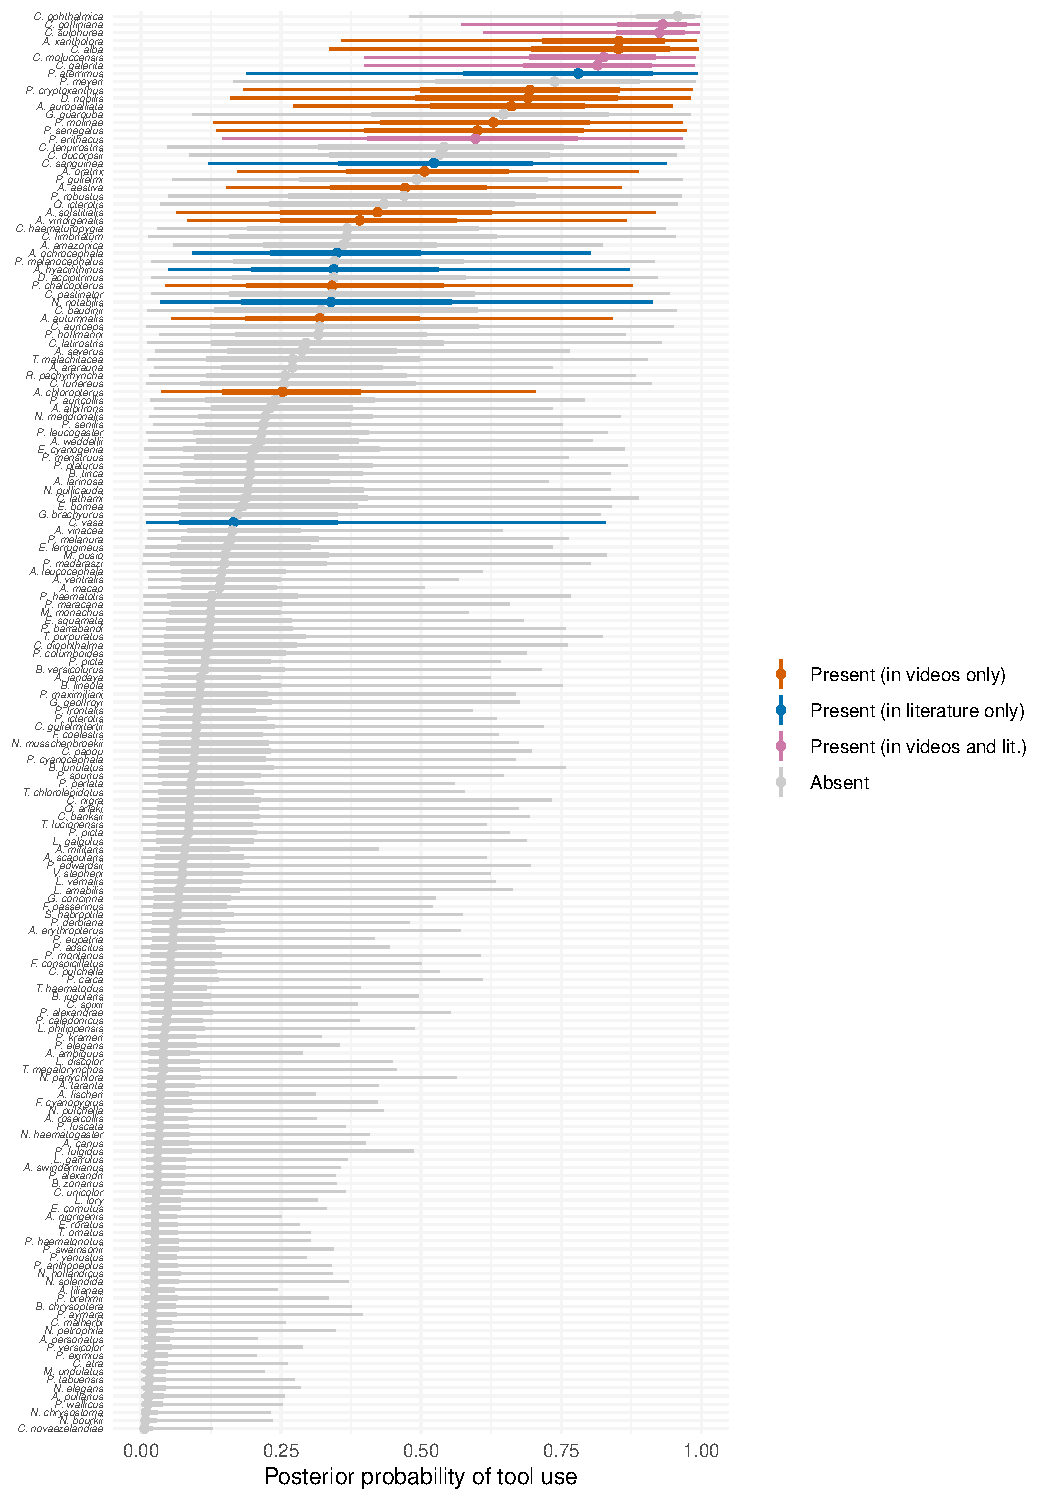
\includegraphics{manuscript_files/figure-latex/plotSurvCure1-1.pdf}
\caption{\label{fig:plotSurvCure1}\emph{Posterior predicted probabilities of tool use for
each species from our phylogenetic survival cure model.} Points are posterior
medians and lines are 50\% and 95\% credible intervals. Total \emph{n} =
174 species.}
\end{figure}






\begin{figure}
\centering
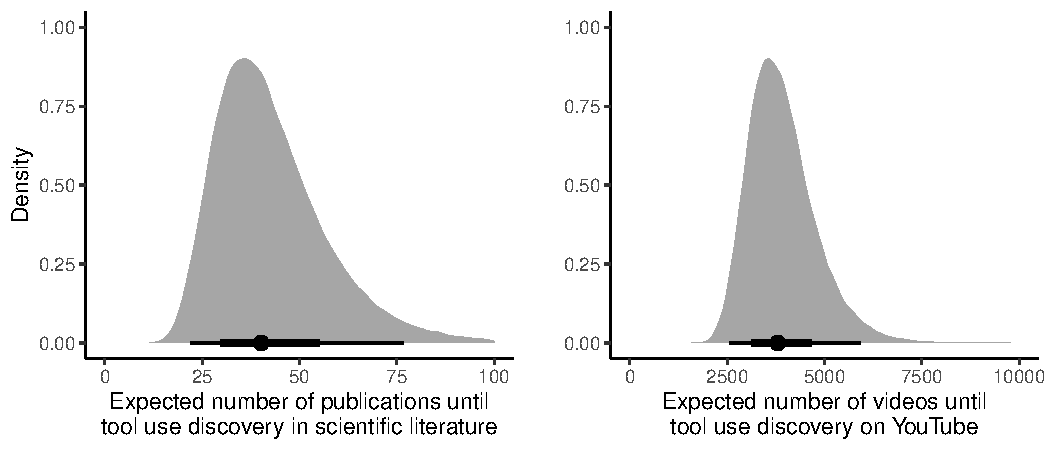
\includegraphics{manuscript_files/figure-latex/plotSurvCure2-1.pdf}
\caption{\label{fig:plotSurvCure2}\emph{Expected number of published papers and videos until
tool use discovery, according to the survival component of the phylogenetic
survival cure model.} Densities are full posterior distributions, points are
posterior medians, and lines are 50\% and 95\% credible intervals.}
\end{figure}

The posterior probabilities shown in Figure \ref{fig:plotSurvCure1} are
estimated with uncertainty, so it is difficult to ``identify'' any particular
species as having an undetected capacity for tool use. Nevertheless, taking the
sum of all the posterior probabilities for the
149 species without
observed evidence of tool use, we can estimate that around
26 of those species are likely to be
undetected tool users (median sum of probabilities =
25.68, 95\% CI
{[}15.15
41.33{]}). When combined with the
species known to use tools, this implies that between 11\% and 17\% of extant
parrot species may be tool users.

\hypertarget{implications-for-the-evolutionary-drivers-and-origins-of-tool-use}{%
\subsection{Implications for the evolutionary drivers and origins of tool use}\label{implications-for-the-evolutionary-drivers-and-origins-of-tool-use}}

The predicted probabilities from our phylogenetic survival cure model have
implications for inferences about the evolutionary drivers and origins of tool
use in the parrot order. Regarding the drivers of tool use hypothesised in
Figure \ref{fig:plotDAG}, the phylogenetic survival cure model revealed that
encephalisation quotient strongly positively predicted the probability of tool
use (median posterior log odds slope = 1.12, 95\%
CI {[}0.39
2.00{]}; total \emph{n} = 174
species; Figure \ref{fig:plotSurvCure4}). This helps explain the ranking in
Figure \ref{fig:plotSurvCure1}: the blue-eyed cockatoo has the largest relative
brain size in the dataset. We also found that feeding generalist species were
slightly more likely to be tool users, though the posterior difference between
generalists and specialists was quite uncertain (median posterior log odds
difference = 0.33, 95\% CI {[}
-1.13 1.76{]}; total
\emph{n} = 174 species). These results from the survival cure model
differed from the results of models fitted to pre-video-survey and
post-video-survey data without the survival cure component, which found no
effect of relative brain size and no difference between feeding strategies,
respectively (Figure \ref{fig:plotComparison}).













\begin{figure}
\centering
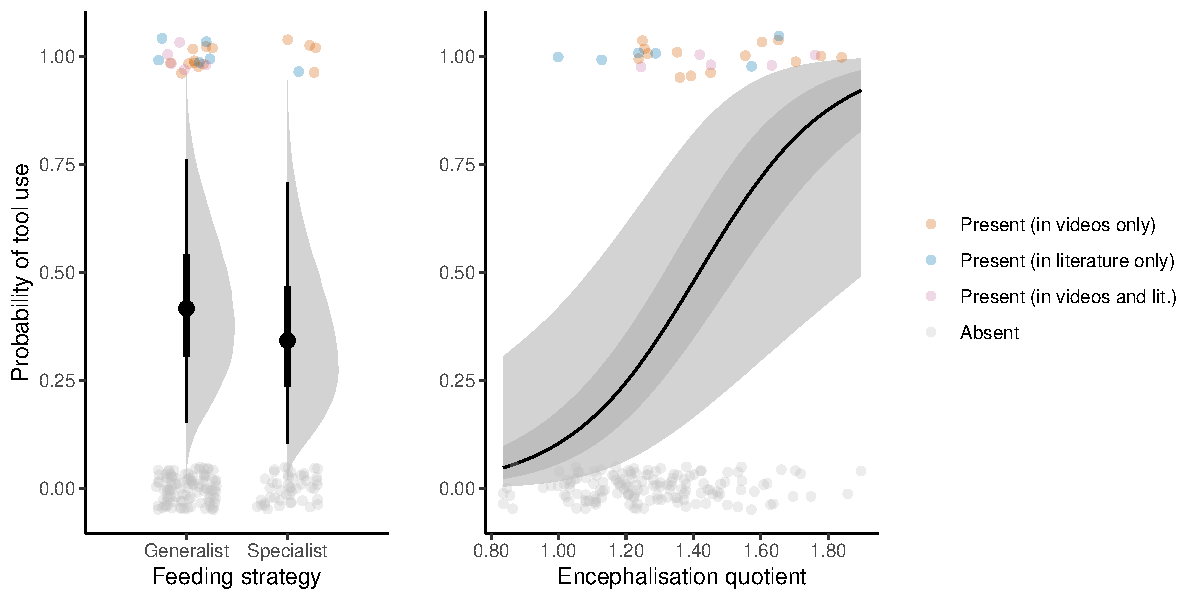
\includegraphics{manuscript_files/figure-latex/plotSurvCure4-1.pdf}
\caption{\label{fig:plotSurvCure4}\emph{Posterior predictions for the effects of feeding
strategy and encephalisation quotient on the probability of tool use from the
phylogenetic survival cure model.} In the left plot, points and lines represent
posterior medians and 50\% and 95\% credible intervals, with densities
representing full posterior distributions. In the right plot, the line and
shaded areas represent the posterior median regression line with 50\% and 95\%
credible intervals. In both plots, individual species are coloured according to
the presence / absence of tool use in the video survey and the scientific
literature. Total \emph{n} = 174 species, generalist \emph{n} =
121 species, specialist \emph{n} =
53 species.}
\end{figure}

Regarding the origins of tool use, we fitted exploratory ancestral state
reconstruction models to the pre-video-survey data, the post-video-survey data,
and the predicted probabilities from the phylogenetic survival cure model. The
discoveries from our video survey and from our phylogenetic modelling increased
the likelihood that the capacity for tool use was present in the most recent
common ancestors for several parrot genera. These include the most recent common
ancestor of amazon parrots native to the Americas (\emph{Amazona}), the most recent
common ancestor of the true white cockatoos and corellas found in South East
Asia and Australasia (\emph{Cacatua}), the most recent common ancestor of the kea and
the kākā from New Zealand (\emph{Nestor}), and the most recent common ancestor for
the \emph{Poicephalus} genus native to Africa (Table \ref{tab:tableASR};
Figures \ref{fig:plotASR1} - \ref{fig:plotASR3}).







\begin{table}[tbp]

\begin{center}
\begin{threeparttable}

\caption{\label{tab:tableASR}Estimated probabilities of tool use for most recent common
ancestors of several parrot genera. \emph{Probabilities estimated using exploratory
ancestral state reconstruction models fitted to the pre-video-survey data,
post-video-survey data, and predicted probabilities from the phylogenetic
survival cure model. Total} n \emph{= 174 species.}}

\begin{tabular}{llll}
\toprule
Genus & \multicolumn{1}{c}{Pre-video-survey} & \multicolumn{1}{c}{Post-video-survey} & \multicolumn{1}{c}{Survival cure probabilities}\\
\midrule
\textit{Amazona} & 0.06, 95\% CI [0.01 0.17] & 0.21, 95\% CI [0.04 0.66] & 0.48, 95\% CI [0.05 0.84]\\
\textit{Cacatua} & 0.08, 95\% CI [0.03 0.20] & 0.17, 95\% CI [0.03 0.45] & 0.81, 95\% CI [0.23 0.99]\\
\textit{Nestor} & 0.11, 95\% CI [0.05 0.29] & 0.21, 95\% CI [0.12 0.37] & 0.53, 95\% CI [0.29 0.66]\\
\textit{Poicephalus} & 0.06, 95\% CI [0.02 0.11] & 0.19, 95\% CI [0.12 0.41] & 0.72, 95\% CI [0.16 0.90]\\
\bottomrule
\end{tabular}

\end{threeparttable}
\end{center}

\end{table}

\hypertarget{discussion}{%
\section{Discussion}\label{discussion}}

Since the earliest anecdotes of parrots using tools by Wallace in the 1880s\textsuperscript{59} and more systematic anecdotal reports in the 1970s\textsuperscript{60},
only 11 parrot species (3\% of all extant parrots) have been documented as tool
users in the scientific literature. Our study collated data from a digital video
platform and revealed capabilities for self-care tool use in 17 additional
parrot species, more than doubling the overall count of tool-using parrots to
28 species (7\%). These species consisted of cockatoos (\emph{Cacatuidae}), Old World
parrots (\emph{Psittacinae}), and neotropical parrots (\emph{Arinae}). Beyond the video
survey, the strong phylogenetic signal in our dataset allowed us to use
phylogenetic information, along with other variables, to infer the unobserved
probabilities of tool use across the parrot order. Our phylogenetic survival
cure model incorporated information on phylogenetic history, research effort,
relative brain size, and feeding specialisation to rank parrot species that were
most likely to be undetected tool users. The sum of probabilities from this
model implied that between 15 and 41 of the species without evidence of tool use
are likely to have an unobserved capacity for tool use, suggesting that the true
proportion of tool users in the parrot order may be as high as 17\%.

All instances of tool use in our video survey met the established criteria for
tool use in the literature: the manipulation of an unattached object as an
extension of the animal's body to achieve a goal\textsuperscript{10}. However, a
striking feature of the dataset is that the 17 additional species identified in
the video survey were exclusively observed using tools for self-scratching.
While parrots in the wild use tools to achieve a variety of goals, including
extractive foraging and courtship\textsuperscript{34,35,38,61}, parrots in captivity rarely ever require tools in an environment
where food is readily available and there is little or no competition for mates.
Instead, the most commonly observed form of tool use in captive parrots is
self-scratching. It could be argued that self-scratching is a more cognitively
simple form of tool use than extractive foraging as it is egocentric, meaning
that the tool is directed towards oneself rather than an external object.
Nevertheless, self-scratching meets the definition for a more complex type of
embodied tool use known as `tooling', the deliberate generation of a mechanical
interface by using an object to manipulate another target or surface\textsuperscript{62}. In our dataset, most self-scratching tooling instances involved
manipulating the tool while keeping the body still, suggesting that these were
goal-directed, deliberate movements by individuals. Moreover, the fact that we
found strong phylogenetic clustering of self-scratching tool use from the video
survey with other examples of tool use from the literature supports a common
underlying cognitive mechanism. In line with this, some of the species of
parrots that use tools for self-scratching in captivity also use tools for other
purposes in the wild\textsuperscript{30,31,34,38}. For
these reasons, we believe that self-care tool use in captivity is no less
indicative of a cognitive capacity for tool use than other tool behaviours in
the wild or in captivity. Indeed, if this is not the case, then the field will
need to re-evaluate current working definitions of true tool use and their
implications for animal cognition. This justifies our use of self-scratching,
alongside other wild observations of tool use, to make claims about the
evolutionary drivers and origins of technical intelligence in the parrot order.

Our data raise the question of why such a wide range of parrot species exhibit
self-scratching tool use behaviours in captive environments. It is possible that
these self-care behaviours emerge more often in captivity because pet parrots
are kept with few or no conspecifics, and therefore must innovate tool use to
preen inaccessible body areas, such as their heads and necks, which would have
been otherwise preened by flock members. This may indicate that human
interaction and allopreening in the absence of a conspecific is insufficient for
pet parrots, as suggested by studies on welfare and chronic stress in lone
captive parrots\textsuperscript{63--66}. Beyond
social isolation in captivity, other factors that reduce preening efficacy by an
individual might also lead to the innovation of self-care tooling: for example,
a captive kea housed with conspecifics in a naturalistic environment was shown
to have innovated the use of a pebble tool for self-care likely as a consequence
of a missing upper mandible\textsuperscript{31}. These behaviours might therefore be
innovated by individuals when ecologically necessary. Critically, however, a
capacity to innovate a behaviour such as tool use must exist in a species in
order to manifest in any environment, whether that be captive or in the wild.
The fact that only a subset of parrot species are innovating self-care tooling
in response to their captive setting and that self-care tooling is predicted by
phylogenetic history and encephalisation strongly suggests that self-scratching
indicates a capacity to produce tool use, which is expressed in different ways
in captive and wild settings.

Our findings have a number of important implications. First, our findings show
that current research effort in the scientific literature is insufficient to
capture the real world occurrence of parrot tool use. If the scientific
literature had sampled the natural world sufficiently, we would expect to see
close correspondence between those species reported as tool users in the
literature and those species the public have filmed performing tool use.
Instead, we discovered a large discrepancy between these two data sources, both
in the prevalence of tool use and the species identified, likely due to the
numerous difficulties inherent to conducting observations in the wild. This
raises the possibility that other rare behaviours remain yet to be discovered in
the scientific literature.

Second, in terms of the evolution of tool use in parrots, our study challenges a
key assumption made in the literature to date: that only a minority of parrots
are tool users\textsuperscript{30,31,34,37,38}.
The paucity of evidence for tool use across parrots in the literature initially
implied that the capacity for tool use may have evolved independently in
different parrot species. Our discovery of the widespread distribution of tool
use across the parrot phylogeny, along with the strong phylogenetic signal in
this expanded dataset, challenges this and suggests that, at least for some
parrot clades, the capacity for tool use might be a homologous trait that has
been evolutionarily conserved. Our exploratory ancestral state reconstruction
analysis provides preliminary support for this hypothesis, revealing an
increased probability of the capacity for tool use among the most recent common
ancestors for the \emph{Amazona}, \emph{Cacatua}, \emph{Nestor}, and \emph{Poicephalus} genera. The
complexity of tool use behaviour that such a basic capacity might afford, and
the conditions under which it emerges in the wild, are yet to be established.
However, even at this preliminary stage, our analysis raises an alternative
hypothesis for the observed tool use in \emph{Cacatua}\textsuperscript{30,38}
and \emph{Nestor}\textsuperscript{26--29,31,34}, namely that tool behaviours have arisen due to the
common ancestor having the capacity to use tools, rather than from independent
evolution or behavioural innovation within species.

Third, our results support existing theories of the drivers of tool use. We
found that encephalisation was strongly positively related to the probability of
tool use in our phylogenetic model, supporting previous theories linking
relative brain size to increased tool innovation in birds\textsuperscript{12--14} and primates\textsuperscript{67}. We acknowledge that
encephalisation quotient is not a perfect measure due to measurement error and
challenges with interpretation\textsuperscript{3,4}. However, encephalisation
quotient has much greater coverage across the parrot phylogeny than more
fine-grained measures like whole neuron count\textsuperscript{68} and there is no reason
to think that measurement error would produce the consistent patterns across our
study and prior work. To understand the causal mechanisms responsible for these
relationships, we encourage further work on the specific neural correlates of
technical intelligence in parrots, e.g.,\textsuperscript{69}. In our phylogenetic
model, we also found that tool use was somewhat more likely among feeding
generalists compared to feeding specialists, although this difference was
uncertain. This trend supports previous suggestions that increased cognitive
abilities and technical innovation rates are required to expand a generalist
species' dietary niche\textsuperscript{18,20,70}. However, the trend contradicts theories linking tool use to
dietary specialisation, whereby species eating specific foods that require
extractive foraging have higher cognitive ability and are especially prone to
using tools\textsuperscript{20}.

A potential concern with data originating from digital video platforms is its
reliability\textsuperscript{23,71--75}.
In particular, the self-care tool use instances detected in our video survey
might be attributable to training or unintentional cueing by the birds' owners.
However, there was little evidence to suggest that the observations of
self-scratching tool use in the video survey were merely unintentional accidents
or explicitly trained behaviours. Individual parrots often used tools slowly and
repetitively over long periods of time, even across multiple different videos,
suggesting that their behaviour was not random or accidental\textsuperscript{74}.
Parrots preferentially employed self-scratching tools on areas of their body
that were otherwise inaccessible, with 96\% of all instances involving scratching
of the head or neck, suggesting intentional tool use. For 60\% of the species in
the video survey, we found two or more videos of repetitive and sustained
scratching by different individuals of the same species in separate households,
suggesting that the manipulations were intentional and recurring events that did
not represent unusual stereotypies of any single individual. Regarding the
possibility of training or cueing from owners, over half of the videos contained
no evidence of human interaction aside from filming the behaviour. Humans only
handed parrots their tools in two of the videos, and none of the videos featured
owners directly rewarding tool use behaviours with food. It is unlikely that
owners would specifically train parrots to scratch themselves with tools.
Finally, the high levels of phylogenetic signal in our data provide strong
evidence that the observations from our video survey reflect
biologically-endowed capacities for tool use rather than accidental or trained
behaviours, which would likely appear uniformly across the phylogeny.
Nevertheless, future work using data such as this should choose target
behaviours carefully and examine videos for evidence of training or cueing.

While missing data imputation is becoming more common in phylogenetic
analyses\textsuperscript{76}, the important distinction between absence of
evidence and evidence of absence has not been given as much attention. Our
phylogenetic analysis provides one approach to this problem by distinguishing
between true absences of tool use and absences of tool use due to a lack of
research effort in the scientific literature or in videos. To achieve this, we
explicitly modelled the measurement of the outcome variable along a research
effort time series, such that species with lower research effort in the
literature or in videos were likely to be censored. In line with our causal
model, we also included relative brain size, feeding strategy, and phylogenetic
history as predictors of unobserved tool use. We encourage researchers to test
this model by directing future study efforts towards the parrot species with the
highest probabilities of being undetected tool-users. Future work should also
refine the causal model in Figure \ref{fig:plotDAG} to provide more certain
estimates of tool use probabilities, either by including additional predictor
variables or modelling further causes of measurement error in the taxonomic
record, such as species abundance and geographic accessibility\textsuperscript{22}.

In conclusion, we have shown that the scientific literature has insufficiently
captured the full distribution of tool use in the parrot order. Our
digital video survey identified novel observations of self-care tool use in
several parrot species, more than doubling the number of known tool using parrot
species from 11 to 28. Our phylogenetic model suggested that the true
proportion of parrot tool users could be as high as 17\% of all species in this
order. These discoveries have implications for theories of the evolutionary
drivers and origins of tool use in parrots. Beyond parrot tool use, the
methods used in this study have the potential to be applied to other rarely
observed behaviours, including tool use in other taxa\textsuperscript{77}, rhythmic
entrainment in birds\textsuperscript{78--81},
teasing behaviours in primates\textsuperscript{82}, and tactical deception across all
animals\textsuperscript{83--85}. We hope that these methods
will continue to uncover a diverse array of ephemeral behaviours that have as
yet gone undetected in the scientific literature.

\newpage
\nolinenumbers

\hypertarget{acknowledgements}{%
\section{Acknowledgements}\label{acknowledgements}}

This project was made possible through the support of a grant from the Templeton
World Charity Foundation (A.H.T., X.J.N.). The authors would like to thank
Daniel Sol for providing feedback on a previous version of the manuscript.

\hypertarget{author-contributions}{%
\section{Author Contributions}\label{author-contributions}}

All authors contributed to the conceptualisation of the paper. A.P.M.B., X.J.N.,
and A.H.T. developed the video search methodology. S.C., D.W., and Q.A.D.
developed the statistical models and analysed the data. All the authors wrote
the manuscript and approved the final version for submission.

\hypertarget{declaration-of-interests}{%
\section{Declaration of Interests}\label{declaration-of-interests}}

The authors declare no competing interests.

\newpage

\hypertarget{references}{%
\section{References}\label{references}}

\begingroup

\hypertarget{refs}{}
\begin{CSLReferences}{0}{0}
\leavevmode\vadjust pre{\hypertarget{ref-MacLean2012}{}}%
\CSLLeftMargin{1. }%
\CSLRightInline{MacLean, E.L., Matthews, L.J., Hare, B.A., Nunn, C.L., Anderson, R.C., Aureli, F., Brannon, E.M., Call, J., Drea, C.M., Emery, N.J., et al. (2012). How does cognition evolve? Phylogenetic comparative psychology. Animal Cognition \emph{15}, 223--238. \url{https://doi.org/10.1007/s10071-011-0448-8}.}

\leavevmode\vadjust pre{\hypertarget{ref-Lefebvre2011}{}}%
\CSLLeftMargin{2. }%
\CSLRightInline{Lefebvre, L. (2011). Taxonomic counts of cognition in the wild. Biology Letters \emph{7}, 631--633. \url{https://doi.org/10.1098/rsbl.2010.0556}.}

\leavevmode\vadjust pre{\hypertarget{ref-Logan2018}{}}%
\CSLLeftMargin{3. }%
\CSLRightInline{Logan, C.J., Avin, S., Boogert, N., Buskell, A., Cross, F.R., Currie, A., Jelbert, S., Lukas, D., Mares, R., Navarrete, A.F., et al. (2018). Beyond brain size: Uncovering the neural correlates of behavioral and cognitive specialization. Comparative Cognition \& Behavior Reviews \emph{13}, 55--89. \url{https://doi.org/10.3819/CCBR.2018.130008}.}

\leavevmode\vadjust pre{\hypertarget{ref-Healy2007}{}}%
\CSLLeftMargin{4. }%
\CSLRightInline{Healy, S.D., and Rowe, C. (2007). A critique of comparative studies of brain size. Proceedings of the Royal Society B: Biological Sciences \emph{274}, 453--464. \url{https://doi.org/10.1098/rspb.2006.3748}.}

\leavevmode\vadjust pre{\hypertarget{ref-Powell2017}{}}%
\CSLLeftMargin{5. }%
\CSLRightInline{Powell, L.E., Isler, K., and Barton, R.A. (2017). Re-evaluating the link between brain size and behavioural ecology in primates. Proceedings of the Royal Society B: Biological Sciences \emph{284}, 20171765. \url{https://doi.org/10.1098/rspb.2017.1765}.}

\leavevmode\vadjust pre{\hypertarget{ref-Goodall1964}{}}%
\CSLLeftMargin{6. }%
\CSLRightInline{Goodall, J. (1964). Tool-using and aimed throwing in a community of free-living chimpanzees. Nature \emph{201}, 1264--1266.}

\leavevmode\vadjust pre{\hypertarget{ref-Hunt1996}{}}%
\CSLLeftMargin{7. }%
\CSLRightInline{Hunt, G.R. (1996). Manufacture and use of hook-tools by {N}ew {C}aledonian crows. Nature \emph{379}, 249--251. \url{https://doi.org/10.1038/379249a0}.}

\leavevmode\vadjust pre{\hypertarget{ref-Smolker1997}{}}%
\CSLLeftMargin{8. }%
\CSLRightInline{Smolker, R., Richards, A., Connor, R., Mann, J., and Berggren, P. (1997). Sponge carrying by dolphins ({D}elphinidae, \emph{{T}ursiops} sp.): A foraging specialization involving tool use? Ethology \emph{103}, 454--465. \url{https://doi.org/10.1111/j.1439-0310.1997.tb00160.x}.}

\leavevmode\vadjust pre{\hypertarget{ref-Finn2009}{}}%
\CSLLeftMargin{9. }%
\CSLRightInline{Finn, J.K., Tregenza, T., and Norman, M.D. (2009). Defensive tool use in a coconut-carrying octopus. Current Biology \emph{19}, R1069--R1070. \url{https://doi.org/10.1016/j.cub.2009.10.052}.}

\leavevmode\vadjust pre{\hypertarget{ref-Shumaker2011}{}}%
\CSLLeftMargin{10. }%
\CSLRightInline{Shumaker, R.W., Walkup, K.R., Beck, B.B., and Burghardt, G.M. (2011). Animal tool behavior: The use and manufacture of tools by animals (Johns Hopkins University Press) \url{https://doi.org/10.1353/book.98237}.}

\leavevmode\vadjust pre{\hypertarget{ref-Audet2024}{}}%
\CSLLeftMargin{11. }%
\CSLRightInline{Audet, J.-N., Couture, M., Lefebvre, L., and Jarvis, E.D. (2024). Problem-solving skills are predicted by technical innovations in the wild and brain size in passerines. Nature Ecology \& Evolution \emph{8}, 806--816. \url{https://doi.org/10.1038/s41559-024-02342-7}.}

\leavevmode\vadjust pre{\hypertarget{ref-Lefebvre2002}{}}%
\CSLLeftMargin{12. }%
\CSLRightInline{Lefebvre, L., Nicolakakis, N., and Boire, D. (2002). Tools and brains in birds. Behaviour \emph{139}, 939--973. \url{https://doi.org/10.1163/156853902320387918}.}

\leavevmode\vadjust pre{\hypertarget{ref-Lefebvre1997}{}}%
\CSLLeftMargin{13. }%
\CSLRightInline{Lefebvre, L., Whittle, P., Lascaris, E., and Finkelstein, A. (1997). Feeding innovations and forebrain size in birds. Animal Behaviour \emph{53}, 549--560. \url{https://doi.org/10.1006/anbe.1996.0330}.}

\leavevmode\vadjust pre{\hypertarget{ref-Lefebvre2004}{}}%
\CSLLeftMargin{14. }%
\CSLRightInline{Lefebvre, L., Reader, S.M., and Sol, D. (2004). Brains, innovations and evolution in birds and primates. Brain, Behavior and Evolution \emph{63}, 233--246. \url{https://doi.org/10.1159/000076784}.}

\leavevmode\vadjust pre{\hypertarget{ref-Sol2005}{}}%
\CSLLeftMargin{15. }%
\CSLRightInline{Sol, D., Duncan, R.P., Blackburn, T.M., Cassey, P., and Lefebvre, L. (2005). Big brains, enhanced cognition, and response of birds to novel environments. Proceedings of the National Academy of Sciences \emph{102}, 5460--5465. \url{https://doi.org/10.1073/pnas.0408145102}.}

\leavevmode\vadjust pre{\hypertarget{ref-Sol2009}{}}%
\CSLLeftMargin{16. }%
\CSLRightInline{Sol, D. (2009). Revisiting the cognitive buffer hypothesis for the evolution of large brains. Biology Letters \emph{5}, 130--133. \url{https://doi.org/10.1098/rsbl.2008.0621}.}

\leavevmode\vadjust pre{\hypertarget{ref-Kaplan2020}{}}%
\CSLLeftMargin{17. }%
\CSLRightInline{Kaplan, G. (2020). Play behaviour, not tool using, relates to brain mass in a sample of birds. Scientific Reports \emph{10}, 20437. \url{https://doi.org/10.1038/s41598-020-76572-7}.}

\leavevmode\vadjust pre{\hypertarget{ref-Ducatez2015}{}}%
\CSLLeftMargin{18. }%
\CSLRightInline{Ducatez, S., Clavel, J., and Lefebvre, L. (2015). Ecological generalism and behavioural innovation in birds: Technical intelligence or the simple incorporation of new foods? Journal of Animal Ecology \emph{84}, 79--89. \url{https://doi.org/10.1111/1365-2656.12255}.}

\leavevmode\vadjust pre{\hypertarget{ref-Overington2011}{}}%
\CSLLeftMargin{19. }%
\CSLRightInline{Overington, S.E., Griffin, A.S., Sol, D., and Lefebvre, L. (2011). Are innovative species ecological generalists? A test in {N}orth {A}merican birds. Behavioral Ecology \emph{22}, 1286--1293. \url{https://doi.org/10.1093/beheco/arr130}.}

\leavevmode\vadjust pre{\hypertarget{ref-HenkeVonDerMalsburg2020}{}}%
\CSLLeftMargin{20. }%
\CSLRightInline{Henke-von der Malsburg, J., Kappeler, P.M., and Fichtel, C. (2020). Linking ecology and cognition: Does ecological specialisation predict cognitive test performance? Behavioral Ecology and Sociobiology \emph{74}, 154.}

\leavevmode\vadjust pre{\hypertarget{ref-MettkeHofmann2014}{}}%
\CSLLeftMargin{21. }%
\CSLRightInline{Mettke-Hofmann, C. (2014). Cognitive ecology: Ecological factors, life-styles, and cognition. WIREs Cognitive Science \emph{5}, 345--360. \url{https://doi.org/10.1002/wcs.1289}.}

\leavevmode\vadjust pre{\hypertarget{ref-Ducatez2014}{}}%
\CSLLeftMargin{22. }%
\CSLRightInline{Ducatez, S., and Lefebvre, L. (2014). Patterns of research effort in birds. PLOS ONE \emph{9}, e89955. \url{https://doi.org/10.1371/journal.pone.0089955}.}

\leavevmode\vadjust pre{\hypertarget{ref-Nelson2013}{}}%
\CSLLeftMargin{23. }%
\CSLRightInline{Nelson, X.J., and Fijn, N. (2013). The use of visual media as a tool for investigating animal behaviour. Animal Behaviour \emph{85}, 525--536. \url{https://doi.org/10.1016/j.anbehav.2012.12.009}.}

\leavevmode\vadjust pre{\hypertarget{ref-Krueger2019}{}}%
\CSLLeftMargin{24. }%
\CSLRightInline{Krueger, K., Esch, L., and Byrne, R. (2019). Animal behaviour in a human world: A crowdsourcing study on horses that open door and gate mechanisms. PLOS ONE \emph{14}, 1--20. \url{https://doi.org/10.1371/journal.pone.0218954}.}

\leavevmode\vadjust pre{\hypertarget{ref-Pokharel2022}{}}%
\CSLLeftMargin{25. }%
\CSLRightInline{Pokharel, S.S., Sharma, N., and Sukumar, R. (2022). Viewing the rare through public lenses: Insights into dead calf carrying and other thanatological responses in {A}sian elephants using YouTube videos. Royal Society Open Science \emph{9}, 211740. \url{https://doi.org/10.1098/rsos.211740}.}

\leavevmode\vadjust pre{\hypertarget{ref-Auersperg2009}{}}%
\CSLLeftMargin{26. }%
\CSLRightInline{Auersperg, A.M.I., Gajdon, G.K., and Huber, L. (2009). Kea (\emph{{N}estor notabilis}) consider spatial relationships between objects in the support problem. Biology Letters \emph{5}, 455--458. \url{https://doi.org/10.1098/rsbl.2009.0114}.}

\leavevmode\vadjust pre{\hypertarget{ref-Auersperg2010}{}}%
\CSLLeftMargin{27. }%
\CSLRightInline{Auersperg, A.M.I., Gajdon, G.K., and Huber, L. (2010). Kea, \emph{{N}estor notabilis}, produce dynamic relationships between objects in a second-order tool use task. Animal Behaviour \emph{80}, 783--789. \url{https://doi.org/10.1016/j.anbehav.2010.08.007}.}

\leavevmode\vadjust pre{\hypertarget{ref-Auersperg2011a}{}}%
\CSLLeftMargin{28. }%
\CSLRightInline{Auersperg, A.M.I., Huber, L., and Gajdon, G.K. (2011). Navigating a tool end in a specific direction: Stick-tool use in kea (\emph{{N}estor notabilis}). Biology Letters \emph{7}, 825--828. \url{https://doi.org/10.1098/rsbl.2011.0388}.}

\leavevmode\vadjust pre{\hypertarget{ref-Auersperg2011b}{}}%
\CSLLeftMargin{29. }%
\CSLRightInline{Auersperg, A.M.I., Bayern, A.M.P. von, Gajdon, G.K., Huber, L., and Kacelnik, A. (2011). Flexibility in problem solving and tool use of kea and {N}ew {C}aledonian crows in a multi access box paradigm. PLOS ONE \emph{6}, 1--8. \url{https://doi.org/10.1371/journal.pone.0020231}.}

\leavevmode\vadjust pre{\hypertarget{ref-Auersperg2012}{}}%
\CSLLeftMargin{30. }%
\CSLRightInline{Auersperg, A.M.I., Szabo, B., von Bayern, A.M.P., and Kacelnik, A. (2012). Spontaneous innovation in tool manufacture and use in a {G}offin's cockatoo. Current Biology \emph{22}, R903--R904. \url{https://doi.org/10.1016/j.cub.2012.09.002}.}

\leavevmode\vadjust pre{\hypertarget{ref-Bastos2021}{}}%
\CSLLeftMargin{31. }%
\CSLRightInline{Bastos, A.P., Horváth, K., Webb, J.L., Wood, P.M., and Taylor, A.H. (2021). Self-care tooling innovation in a disabled kea (\emph{{N}estor notabilis}). Scientific Reports \emph{11}, 18035.}

\leavevmode\vadjust pre{\hypertarget{ref-BentleyCondit2010}{}}%
\CSLLeftMargin{32. }%
\CSLRightInline{Bentley-Condit, V., and Smith, E.O. (2010). Animal tool use: Current definitions and an updated comprehensive catalog. Behaviour \emph{147}, 185--32A. \url{https://doi.org/10.1163/000579509X12512865686555}.}

\leavevmode\vadjust pre{\hypertarget{ref-Borsari2005}{}}%
\CSLLeftMargin{33. }%
\CSLRightInline{Borsari, A., and Ottoni, E.B. (2005). Preliminary observations of tool use in captive hyacinth macaws (\emph{{A}nodorhynchus hyacinthinus}). Animal Cognition \emph{8}, 48--52. \url{https://doi.org/10.1007/s10071-004-0221-3}.}

\leavevmode\vadjust pre{\hypertarget{ref-Goodman2018}{}}%
\CSLLeftMargin{34. }%
\CSLRightInline{Goodman, M., Hayward, T., and Hunt, G.R. (2018). Habitual tool use innovated by free-living {N}ew {Z}ealand kea. Scientific Reports \emph{8}, 13935. \url{https://doi.org/10.1038/s41598-018-32363-9}.}

\leavevmode\vadjust pre{\hypertarget{ref-Heinsohn2017}{}}%
\CSLLeftMargin{35. }%
\CSLRightInline{Heinsohn, R., Zdenek, C.N., Cunningham, R.B., Endler, J.A., and Langmore, N.E. (2017). Tool-assisted rhythmic drumming in palm cockatoos shares key elements of human instrumental music. Science Advances \emph{3}, e1602399. \url{https://doi.org/10.1126/sciadv.1602399}.}

\leavevmode\vadjust pre{\hypertarget{ref-Janzen1976}{}}%
\CSLLeftMargin{36. }%
\CSLRightInline{Janzen, M.J., Janzen, D.H., and Pond, C.M. (1976). Tool-using by the {A}frican grey parrot (\emph{{P}sittacus erithacus}). Biotropica \emph{8}, 70.}

\leavevmode\vadjust pre{\hypertarget{ref-Lambert2015}{}}%
\CSLLeftMargin{37. }%
\CSLRightInline{Lambert, M.L., Seed, A.M., and Slocombe, K.E. (2015). A novel form of spontaneous tool use displayed by several captive greater vasa parrots (\emph{{C}oracopsis vasa}). Biology Letters \emph{11}, 20150861. \url{https://doi.org/10.1098/rsbl.2015.0861}.}

\leavevmode\vadjust pre{\hypertarget{ref-OHara2021}{}}%
\CSLLeftMargin{38. }%
\CSLRightInline{O'Hara, M., Mioduszewska, B., Mundry, R., Yohanna, Haryoko, T., Rachmatika, R., Prawiradilaga, D.M., Huber, L., and Auersperg, A.M.I. (2021). Wild {G}offin's cockatoos flexibly manufacture and use tool sets. Current Biology \emph{31}, 4512--4520.e6. \url{https://doi.org/10.1016/j.cub.2021.08.009}.}

\leavevmode\vadjust pre{\hypertarget{ref-Anderson2003}{}}%
\CSLLeftMargin{39. }%
\CSLRightInline{Anderson, P. (2003). A bird in the house: An anthropological perspective on companion parrots. Society \& Animals \emph{11}, 393--418. \url{https://doi.org/10.1163/156853003322796109}.}

\leavevmode\vadjust pre{\hypertarget{ref-Carrete2008}{}}%
\CSLLeftMargin{40. }%
\CSLRightInline{Carrete, M., and Tella, J. (2008). Wild-bird trade and exotic invasions: A new link of conservation concern? Frontiers in Ecology and the Environment \emph{6}, 207--211. \url{https://doi.org/10.1890/070075}.}

\leavevmode\vadjust pre{\hypertarget{ref-Drews2001}{}}%
\CSLLeftMargin{41. }%
\CSLRightInline{Drews, C. (2001). Wild animals and other pets kept in {C}osta {R}ican households: Incidence, species and numbers. Society \& Animals \emph{9}, 107--126. \url{https://doi.org/10.1163/156853001753639233}.}

\leavevmode\vadjust pre{\hypertarget{ref-Kelly2014}{}}%
\CSLLeftMargin{42. }%
\CSLRightInline{Kelly, D., McCarthy, E., Menzel, K., and Engebretson, M. (2014). \href{https://www.avianwelfare.org/issues/overview.htm}{How many captive birds: Are population studies giving us a clear picture?}}

\leavevmode\vadjust pre{\hypertarget{ref-Li2014}{}}%
\CSLLeftMargin{43. }%
\CSLRightInline{Li, L., and Jiang, Z. (2014). International trade of {CITES} listed bird species in {C}hina. PLOS ONE \emph{9}, 1--8. \url{https://doi.org/10.1371/journal.pone.0085012}.}

\leavevmode\vadjust pre{\hypertarget{ref-Su2015}{}}%
\CSLLeftMargin{44. }%
\CSLRightInline{Su, S., Cassey, P., Vall-llosera, M., and Blackburn, T.M. (2015). Going cheap: Determinants of bird price in the {T}aiwanese pet market. PLOS ONE \emph{10}, 1--17. \url{https://doi.org/10.1371/journal.pone.0127482}.}

\leavevmode\vadjust pre{\hypertarget{ref-Young2012}{}}%
\CSLLeftMargin{45. }%
\CSLRightInline{Young, A.M., Hobson, E.A., Lackey, L.B., and Wright, T.F. (2012). Survival on the ark: Life-history trends in captive parrots. Animal Conservation \emph{15}, 28--43. \url{https://doi.org/10.1111/j.1469-1795.2011.00477.x}.}

\leavevmode\vadjust pre{\hypertarget{ref-Flammer2001}{}}%
\CSLLeftMargin{46. }%
\CSLRightInline{Flammer, K., Whitt-Smith, D., and Papich, M. (2001). Plasma concentrations of doxycycline in selected psittacine birds when administered in water for potential treatment of \emph{{C}hlamydophila psittaci} infection. Journal of Avian Medicine and Surgery \emph{15}, 276--282. \url{https://doi.org/10.1647/1082-6742(2001)015\%5B0276:PCODIS\%5D2.0.CO;2}.}

\leavevmode\vadjust pre{\hypertarget{ref-Iwaniuk2005}{}}%
\CSLLeftMargin{47. }%
\CSLRightInline{Iwaniuk, A.N., Dean, K.M., and Nelson, J.E. (2005). Interspecific allometry of the brain and brain regions in parrots ({P}sittaciformes): Comparisons with other birds and primates. Brain, Behavior and Evolution \emph{65}, 40--59.}

\leavevmode\vadjust pre{\hypertarget{ref-Mazengenya2018}{}}%
\CSLLeftMargin{48. }%
\CSLRightInline{Mazengenya, P., Bhagwandin, A., Manger, P.R., and Ihunwo, A.O. (2018). Putative adult neurogenesis in {O}ld {W}orld parrots: The {C}ongo {A}frican grey parrot (\emph{{P}sittacus erithacus}) and {T}imneh grey parrot (\emph{{P}sittacus timneh}). Frontiers in Neuroanatomy \emph{12}, 7. \url{https://doi.org/10.3389/fnana.2018.00007}.}

\leavevmode\vadjust pre{\hypertarget{ref-Olkowicz2016}{}}%
\CSLLeftMargin{49. }%
\CSLRightInline{Olkowicz, S., Kocourek, M., Lučan, R.K., Porteš, M., Fitch, W.T., Herculano-Houzel, S., and Němec, P. (2016). Birds have primate-like numbers of neurons in the forebrain. Proceedings of the National Academy of Sciences \emph{113}, 7255--7260. \url{https://doi.org/10.1073/pnas.1517131113}.}

\leavevmode\vadjust pre{\hypertarget{ref-Schuck2008}{}}%
\CSLLeftMargin{50. }%
\CSLRightInline{Schuck-Paim, C., Alonso, W.J., and Ottoni, E.B. (2008). Cognition in an ever-changing world: Climatic variability is associated with brain size in neotropical parrots. Brain, Behavior and Evolution \emph{71}, 200--215. \url{https://doi.org/10.1159/000119710}.}

\leavevmode\vadjust pre{\hypertarget{ref-Silva2017}{}}%
\CSLLeftMargin{51. }%
\CSLRightInline{Silva, T., Guzmán, A., Urantówka, A.D., and Mackiewicz, P. (2017). A new parrot taxon from the {Y}ucat{á}n {P}eninsula, {M}exico---its position within genus \emph{{A}mazona} based on morphology and molecular phylogeny. PeerJ \emph{5}, e3475. \url{https://doi.org/10.7717/peerj.3475}.}

\leavevmode\vadjust pre{\hypertarget{ref-Wilman2016}{}}%
\CSLLeftMargin{52. }%
\CSLRightInline{Wilman, H., Belmaker, J., Simpson, J., Rosa, C. de la, Rivadeneira, M.M., and Jetz, W. (2016). EltonTraits 1.0: Species-level foraging attributes of the world's birds and mammals. \url{https://doi.org/10.6084/m9.figshare.c.3306933.v1}.}

\leavevmode\vadjust pre{\hypertarget{ref-Jetz2012}{}}%
\CSLLeftMargin{53. }%
\CSLRightInline{Jetz, W., Thomas, G.H., Joy, J.B., Hartmann, K., and Mooers, A.O. (2012). The global diversity of birds in space and time. Nature \emph{491}, 444--448.}

\leavevmode\vadjust pre{\hypertarget{ref-Seed2010}{}}%
\CSLLeftMargin{54. }%
\CSLRightInline{Seed, A., and Byrne, R. (2010). Animal tool-use. Current Biology \emph{20}, R1032--R1039. \url{https://doi.org/10.1016/j.cub.2010.09.042}.}

\leavevmode\vadjust pre{\hypertarget{ref-Bercovitz1987}{}}%
\CSLLeftMargin{55. }%
\CSLRightInline{Bercovitz, A.B. (1987). Avian sex identification techniques. In Companion bird medicine, E. W. Burr, ed. (Iowa State University Press).}

\leavevmode\vadjust pre{\hypertarget{ref-Hoyo2011}{}}%
\CSLLeftMargin{56. }%
\CSLRightInline{Hoyo, J.D., and Bierregaard, R. (2011). Handbook of the birds of the world (Lynx Edicions).}

\leavevmode\vadjust pre{\hypertarget{ref-Amico2018}{}}%
\CSLLeftMargin{57. }%
\CSLRightInline{Amico, M., and Van Keilegom, I. (2018). Cure models in survival analysis. Annual Review of Statistics and Its Application \emph{5}, 311--342. \url{https://doi.org/10.1146/annurev-statistics-031017-100101}.}

\leavevmode\vadjust pre{\hypertarget{ref-Schmidt1989}{}}%
\CSLLeftMargin{58. }%
\CSLRightInline{Schmidt, P., and Witte, A.D. (1989). Predicting criminal recidivism using {``split population''} survival time models. Journal of Econometrics \emph{40}, 141--159. \url{https://doi.org/10.1016/0304-4076(89)90034-1}.}

\leavevmode\vadjust pre{\hypertarget{ref-Wallace1869}{}}%
\CSLLeftMargin{59. }%
\CSLRightInline{Wallace, A.R. (1869). The {M}alay {A}rchipelago: The land of the orang-utan and the bird of paradise; a narrative of travel, with the studies of man and nature (MacMillan; Co.).}

\leavevmode\vadjust pre{\hypertarget{ref-Goodall1971}{}}%
\CSLLeftMargin{60. }%
\CSLRightInline{Goodall, J. (1971). Tool-using in primates and other vertebrates. In Advances in the study of behavior., D. S. Lehrman, R. A. Hinde, and E. Shaw, eds. (Academic Press), pp. 195--249. \url{https://doi.org/10.1016/S0065-3454(08)60157-6}.}

\leavevmode\vadjust pre{\hypertarget{ref-Wood1984}{}}%
\CSLLeftMargin{61. }%
\CSLRightInline{Wood, G.A. (1984). Tool use by the palm cockatoo \emph{{P}robosciger aterrimus} during display. Corella \emph{8}, 94--95.}

\leavevmode\vadjust pre{\hypertarget{ref-Fragaszy2018}{}}%
\CSLLeftMargin{62. }%
\CSLRightInline{Fragaszy, D.M., and Mangalam, M. (2018). Tooling. In Advances in the study of behavior., M. Naguib, L. Barrett, S. D. Healy, J. Podos, L. W. Simmons, and M. Zuk, eds. (Academic Press), pp. 177--241. \url{https://doi.org/10.1016/bs.asb.2018.01.001}.}

\leavevmode\vadjust pre{\hypertarget{ref-Aydinonat2014}{}}%
\CSLLeftMargin{63. }%
\CSLRightInline{Aydinonat, D., Penn, D.J., Smith, S., Moodley, Y., Hoelzl, F., Knauer, F., and Schwarzenberger, F. (2014). Social isolation shortens telomeres in {A}frican {G}rey parrots (\emph{{P}sittacus erithacus erithacus}). PLOS ONE \emph{9}, e93839.}

\leavevmode\vadjust pre{\hypertarget{ref-Engebretson2006}{}}%
\CSLLeftMargin{64. }%
\CSLRightInline{Engebretson, M. (2006). The welfare and suitability of parrots as companion animals: A review. Animal Welfare \emph{15}, 263--276. \url{https://doi.org/10.1017/S0962728600030475}.}

\leavevmode\vadjust pre{\hypertarget{ref-Mason2010}{}}%
\CSLLeftMargin{65. }%
\CSLRightInline{Mason, G.J. (2010). Species differences in responses to captivity: Stress, welfare and the comparative method. Trends in Ecology \& Evolution \emph{25}, 713--721. \url{https://doi.org/10.1016/j.tree.2010.08.011}.}

\leavevmode\vadjust pre{\hypertarget{ref-Meehan2003}{}}%
\CSLLeftMargin{66. }%
\CSLRightInline{Meehan, C., Garner, J., and Mench, J. (2003). Isosexual pair housing improves the welfare of young amazon parrots. Applied Animal Behaviour Science \emph{81}, 73--88. \url{https://doi.org/10.1016/S0168-1591(02)00238-1}.}

\leavevmode\vadjust pre{\hypertarget{ref-Reader2002}{}}%
\CSLLeftMargin{67. }%
\CSLRightInline{Reader, S.M., and Laland, K.N. (2002). Social intelligence, innovation, and enhanced brain size in primates. Proceedings of the National Academy of Sciences \emph{99}, 4436--4441. \url{https://doi.org/10.1073/pnas.062041299}.}

\leavevmode\vadjust pre{\hypertarget{ref-Sol2022}{}}%
\CSLLeftMargin{68. }%
\CSLRightInline{Sol, D., Olkowicz, S., Sayol, F., Kocourek, M., Zhang, Y., Marhounová, L., Osadnik, C., Corssmit, E., Garcia-Porta, J., Martin, T.E., et al. (2022). Neuron numbers link innovativeness with both absolute and relative brain size in birds. Nature Ecology \& Evolution \emph{6}, 1381--1389.}

\leavevmode\vadjust pre{\hypertarget{ref-Alvarez2020}{}}%
\CSLLeftMargin{69. }%
\CSLRightInline{Cabrera-Álvarez, M.J., and Clayton, N.S. (2020). Neural processes underlying tool use in humans, macaques, and corvids. Frontiers in Psychology \emph{11}, 560669. \url{https://doi.org/10.3389/fpsyg.2020.560669}.}

\leavevmode\vadjust pre{\hypertarget{ref-HenkeVonDerMalsburg2021}{}}%
\CSLLeftMargin{70. }%
\CSLRightInline{Henke-von der Malsburg, J., Kappeler, P.M., and Fichtel, C. (2021). Linking cognition to ecology in wild sympatric mouse lemur species. Proceedings of the Royal Society B: Biological Sciences \emph{288}, 20211728. \url{https://doi.org/10.1098/rspb.2021.1728}.}

\leavevmode\vadjust pre{\hypertarget{ref-Auersperg2020}{}}%
\CSLLeftMargin{71. }%
\CSLRightInline{Auersperg, A.M.I., Schwing, R., Mioduszewska, B., O'Hara, M., and Huber, L. (2020). Do puffins use tools? Proceedings of the National Academy of Sciences \emph{117}, 11859--11859. \url{https://doi.org/10.1073/pnas.2001988117}.}

\leavevmode\vadjust pre{\hypertarget{ref-DechaumeMoncharmont2020}{}}%
\CSLLeftMargin{72. }%
\CSLRightInline{Dechaume-Moncharmont, F.-X. (2020). Touchy matter: The delicate balance between {M}organ's canon and open-minded description of advanced cognitive skills in the animal. Peer Community in Ecology, 100042. \url{https://doi.org/10.24072/pci.ecology.100042}.}

\leavevmode\vadjust pre{\hypertarget{ref-Farrar2020}{}}%
\CSLLeftMargin{73. }%
\CSLRightInline{Farrar, B.G. (2020). Evidence of tool use in a seabird? PsyArXiv. \url{https://doi.org/10.31234/osf.io/463hk}.}

\leavevmode\vadjust pre{\hypertarget{ref-Sandor2020}{}}%
\CSLLeftMargin{74. }%
\CSLRightInline{Sándor, K., and Miklósi, Á. (2020). How to report anecdotal observations? A new approach based on a lesson from "puffin tool use". Frontiers in Psychology \emph{11}, 555487. \url{https://doi.org/10.3389/fpsyg.2020.555487}.}

\leavevmode\vadjust pre{\hypertarget{ref-vonBayern2020}{}}%
\CSLLeftMargin{75. }%
\CSLRightInline{von Bayern, A.M., Jacobs, I., and Osvath, M. (2020). Tool-using puffins prickle the puzzle of cognitive evolution. Proceedings of the National Academy of Sciences \emph{117}, 2737--2739. \url{https://doi.org/10.1073/pnas.1922117117}.}

\leavevmode\vadjust pre{\hypertarget{ref-Debastiani2021}{}}%
\CSLLeftMargin{76. }%
\CSLRightInline{Debastiani, V.J., Bastazini, V.A.G., and Pillar, V.D. (2021). Using phylogenetic information to impute missing functional trait values in ecological databases. Ecological Informatics \emph{63}, 101315. \url{https://doi.org/10.1016/j.ecoinf.2021.101315}.}

\leavevmode\vadjust pre{\hypertarget{ref-Hunt2013}{}}%
\CSLLeftMargin{77. }%
\CSLRightInline{Hunt, G.R., Gray, R.D., and Taylor, A.H. (2013). Why is tool use rare in animals? In Tool use in animals: Cognition and ecology, C. M. Sanz, J. Call, and C. Boesch, eds. (Cambridge University Press), pp. 89--118. \url{https://doi.org/10.1017/CBO9780511894800.007}.}

\leavevmode\vadjust pre{\hypertarget{ref-Benichov2016}{}}%
\CSLLeftMargin{78. }%
\CSLRightInline{Benichov, J.I., Globerson, E., and Tchernichovski, O. (2016). Finding the beat: From socially coordinated vocalizations in songbirds to rhythmic entrainment in humans. Frontiers in Human Neuroscience \emph{10}. \url{https://doi.org/10.3389/fnhum.2016.00255}.}

\leavevmode\vadjust pre{\hypertarget{ref-Patel2009}{}}%
\CSLLeftMargin{79. }%
\CSLRightInline{Patel, A.D., Iversen, J.R., Bregman, M.R., and Schulz, I. (2009). Experimental evidence for synchronization to a musical beat in a nonhuman animal. Current Biology \emph{19}, 827--830. \url{https://doi.org/10.1016/j.cub.2009.03.038}.}

\leavevmode\vadjust pre{\hypertarget{ref-tenCate2016}{}}%
\CSLLeftMargin{80. }%
\CSLRightInline{ten Cate, C., Spierings, M., Hubert, J., and Honing, H. (2016). Can birds perceive rhythmic patterns? A review and experiments on a songbird and a parrot species. Frontiers in Psychology \emph{7}. \url{https://doi.org/10.3389/fpsyg.2016.00730}.}

\leavevmode\vadjust pre{\hypertarget{ref-Wilson2016}{}}%
\CSLLeftMargin{81. }%
\CSLRightInline{Wilson, M., and Cook, P.F. (2016). Rhythmic entrainment: Why humans want to, fireflies can't help it, pet birds try, and sea lions have to be bribed. Psychonomic Bulletin \& Review \emph{23}, 1647--1659. \url{https://doi.org/10.3758/s13423-016-1013-x}.}

\leavevmode\vadjust pre{\hypertarget{ref-Eckert2020}{}}%
\CSLLeftMargin{82. }%
\CSLRightInline{Eckert, J., Winkler, S.L., and Cartmill, E.A. (2020). Just kidding: The evolutionary roots of playful teasing. Biology Letters \emph{16}, 20200370. \url{https://doi.org/10.1098/rsbl.2020.0370}.}

\leavevmode\vadjust pre{\hypertarget{ref-BroJorgensen2010}{}}%
\CSLLeftMargin{83. }%
\CSLRightInline{Bro-Jørgensen, J., and Pangle, W.M. (2010). Male topi antelopes alarm snort deceptively to retain females for mating. The American Naturalist \emph{176}, E33--E39. \url{https://doi.org/10.1086/653078}.}

\leavevmode\vadjust pre{\hypertarget{ref-Byrne1988}{}}%
\CSLLeftMargin{84. }%
\CSLRightInline{Byrne, R.W., and Whiten, A. (1988). Toward the next generation in data quality: A new survey of primate tactical deception. Behavioral and Brain Sciences \emph{11}, 267--273. \url{https://doi.org/10.1017/S0140525X00049955}.}

\leavevmode\vadjust pre{\hypertarget{ref-Byrne1991}{}}%
\CSLLeftMargin{85. }%
\CSLRightInline{Byrne, R.W., and Whiten, A. (1991). Computation and mindreading in primate tactical deception. In Natural theories of mind: Evolution, development and simulation of everyday mindreading, A. Whiten, ed. (Basil Blackwell), pp. 127--141.}

\leavevmode\vadjust pre{\hypertarget{ref-GlobalGfkSurvey}{}}%
\CSLLeftMargin{86. }%
\CSLRightInline{\href{http://www.gfk.com/global-studies/global-studies-pet-ownership}{Global GfK survey: Pet ownership} (2016).}

\leavevmode\vadjust pre{\hypertarget{ref-Jerison1973}{}}%
\CSLLeftMargin{87. }%
\CSLRightInline{Jerison, H.J. (1973). Evolution of the brain and intelligence (Academic Press).}

\leavevmode\vadjust pre{\hypertarget{ref-Paradis2019}{}}%
\CSLLeftMargin{88. }%
\CSLRightInline{Paradis, E., and Schliep, K. (2019). {ape} 5.0: An environment for modern phylogenetics and evolutionary analyses in {R}. Bioinformatics \emph{35}, 526--528. \url{https://doi.org/10.1093/bioinformatics/bty633}.}

\leavevmode\vadjust pre{\hypertarget{ref-McElreath2020}{}}%
\CSLLeftMargin{89. }%
\CSLRightInline{McElreath, R. (2020). \href{http://xcelab.net/rm/statistical-rethinking/}{Statistical rethinking: A {Bayesian} course with examples in {R} and {Stan}, 2nd edition} 2nd ed. (CRC Press).}

\leavevmode\vadjust pre{\hypertarget{ref-Stan2020}{}}%
\CSLLeftMargin{90. }%
\CSLRightInline{Stan Development Team (2020). \href{http://mc-stan.org/}{{RStan}: The {R} interface to {Stan}}.}

\leavevmode\vadjust pre{\hypertarget{ref-phytools}{}}%
\CSLLeftMargin{91. }%
\CSLRightInline{Revell, L.J. (2012). {phytools}: An {R} package for phylogenetic comparative biology (and other things). Methods in Ecology and Evolution \emph{3}, 217--223. \url{https://doi.org/10.1111/j.2041-210X.2011.00169.x}.}

\leavevmode\vadjust pre{\hypertarget{ref-RCoreTeam}{}}%
\CSLLeftMargin{92. }%
\CSLRightInline{R Core Team (2022). \href{https://www.R-project.org/}{R: A language and environment for statistical computing} (R Foundation for Statistical Computing).}

\leavevmode\vadjust pre{\hypertarget{ref-ggtree}{}}%
\CSLLeftMargin{93. }%
\CSLRightInline{Yu, G., Smith, D., Zhu, H., Guan, Y., and Lam, T.T.-Y. (2017). {ggtree}: An {R} package for visualization and annotation of phylogenetic trees with their covariates and other associated data. Methods in Ecology and Evolution \emph{8}, 28--36. \url{https://doi.org/10.1111/2041-210X.12628}.}

\leavevmode\vadjust pre{\hypertarget{ref-Wickham2016}{}}%
\CSLLeftMargin{94. }%
\CSLRightInline{Wickham, H. (2016). \href{https://ggplot2.tidyverse.org}{{ggplot2}: Elegant graphics for data analysis} (Springer-Verlag New York).}

\leavevmode\vadjust pre{\hypertarget{ref-Wilke2020}{}}%
\CSLLeftMargin{95. }%
\CSLRightInline{Wilke, C.O. (2020). \href{https://CRAN.R-project.org/package=cowplot}{{cowplot}: Streamlined plot theme and plot annotations for 'ggplot2'}.}

\leavevmode\vadjust pre{\hypertarget{ref-Landau2021}{}}%
\CSLLeftMargin{96. }%
\CSLRightInline{Landau, W.M. (2021). The targets {R} package: A dynamic {M}ake-like function-oriented pipeline toolkit for reproducibility and high-performance computing. Journal of Open Source Software \emph{6}, 2959. \url{https://doi.org/10.21105/joss.02959}.}

\leavevmode\vadjust pre{\hypertarget{ref-Aust2022}{}}%
\CSLLeftMargin{97. }%
\CSLRightInline{Aust, F., and Barth, M. (2022). \href{https://github.com/crsh/papaja}{{papaja}: {Prepare} reproducible {APA} journal articles with {R Markdown}}.}

\end{CSLReferences}

\endgroup

\newpage
\linenumbers

\hypertarget{star-methods}{%
\section{STAR Methods}\label{star-methods}}

\hypertarget{resource-availability}{%
\subsection{Resource Availability}\label{resource-availability}}

\hypertarget{lead-contact}{%
\subsubsection{Lead contact}\label{lead-contact}}

Further information about resources should be directed to Scott Claessens
(\href{mailto:scott.claessens@gmail.com}{\nolinkurl{scott.claessens@gmail.com}}).

\hypertarget{materials-availability}{%
\subsubsection{Materials availability}\label{materials-availability}}

This study did not generate new unique materials.

\hypertarget{data-and-code-availability}{%
\subsubsection{Data and code availability}\label{data-and-code-availability}}

All data have been deposited on GitHub and are publicly available as of the date
of publication. DOIs are listed in the key resources table.

All original code has been deposited on GitHub and is publicly available as of
the date of publication. DOIs are listed in the key resources table.

\hypertarget{method-details}{%
\subsection{Method Details}\label{method-details}}

\hypertarget{video-searches-and-coding}{%
\subsubsection{Video searches and coding}\label{video-searches-and-coding}}

Our video search was conducted on YouTube in July 2020. Searches were conducted
manually by the first author over a month-long period, using the same IP address
and not logged in with a YouTube user account. Search terms included
``parrot using tool'' and variants (e.g., ``macaw using tool'', ``lorikeet using
tool'', ``parakeet using tool''), ``tool use in parrot'', ``parrot tool use'', ``parrot
scratching itself'' (included after we found several videos demonstrating
self-care tool use in previous searches) and equivalent terms (e.g., ``parrot
preening itself'', ``parrot grooming itself'', ``parrot scratching''). For all
species that did not display results including object manipulation or scratching
behaviours, we also searched the species' common name(s) + ``tool use'', as well
as the species' common name(s) + ``scratching''. We also searched for translations
of the terms ``parrot tool use'' and ``parrot scratching'' in languages for all
countries where bird ownership was reported as \textgreater5\%\textsuperscript{86}, namely,
Turkish, Czech, Polish, French, Italian, Dutch, German, Russian, Spanish,
Portuguese, and Mandarin. Browser search histories were not cleared between
searches.

When we found a relevant video, we also searched for similar content uploaded by
the same person/channel. For each YouTube search conducted, we watched all
relevant videos until we reached five consecutive videos that did not feature
any parrots. At this point, we ended that search and initiated the next search.
In line with previous recommendations\textsuperscript{23}, we planned to exclude any
videos that consisted of four or more shots edited together so as to ensure the
behaviours being observed were not edited or manipulated, but none of the videos
obtained qualified for exclusion.

All videos featuring parrots manipulating objects were investigated for
potential tool use or borderline tool use. We defined tool use as the
manipulation of an unattached object as an extension of the beak or foot to
achieve a goal towards another object, individual, or oneself\textsuperscript{10}.
Borderline tool use was similarly defined, except that it involved the use of an
object that was still attached to a substrate\textsuperscript{54}. For example, if
individuals used a fallen feather or stick for self-scratching this was defined
as tool use, but using one's currently attached tail feathers or cage
furnishings for the same purpose was defined as borderline tool use.
Self-scratching had to involve slow and repeated movements of touching an object
to one's body (or, in the case of borderline tool use, rubbing repetitively
against an attached object\textsuperscript{74}).

All relevant videos were coded for video length, species, tool use presence
(yes/borderline), tool use type (e.g., scratching, feeding), the object being
used (e.g., feather, stick), tool use target, human interaction
(talking or handing object to parrot, holding parrot), and the number of shots
within each video. Our complete dataset also includes the name for each video,
link, subject name, sex (as declared by owner, as most parrot species are not
sexually dimorphic), publishing date, and dates found and coded.

Since YouTube is constantly growing and evolving in both its uploaded content
and its proprietary recommendation algorithms, the same search strategy today
would not return exactly the same videos as our search in July 2020. It is
possible that some videos have since been deleted or more videos of parrot tool
use have since been uploaded. However, this does not affect our conclusions
about the number of parrot species found to use tools in our initial search.

\hypertarget{data-for-parrot-species}{%
\subsubsection{Data for parrot species}\label{data-for-parrot-species}}

We collected data for 194 parrot species (Figures
\ref{fig:plotPhylo2} - \ref{fig:plotPhylo4}). We gathered feeding strategy
data as a dichotomous variable (``generalist'' or ``specialist'') from the
EltonTraits ecological database\textsuperscript{52}. As per the database, specialists
were defined as species whose diet comprised at least 70\% of a single food
source. To calculate relative brain size, we collated data from the literature
for all known body mass (g) and brain mass (g) values across
parrots\textsuperscript{46--51}. For all species for which we obtained body and brain mass data, we
calculated the encephalisation quotient (EQ) using the following
formula\textsuperscript{87}: \(BrainWeight / (0.12 * BodyWeight(\frac{2}{3}))\). We
found body mass and brain mass data for a total of 194 parrot species. This
included all tool-using species in our video dataset, with the exception of
three species: \emph{Diopsittaca nobilis}, \emph{Psittacara erythrogenys}, and \emph{Coracopsis
vasa}. For the latter, we used values for the closely related \emph{Coracopsis
nigra}. The other two species were excluded from the final dataset.

For modelling purposes, we coded research effort in both the scientific
literature and the YouTube videos. For the scientific literature, we
operationalised research effort as the number of papers published for each
species' Latin name up to and including the first paper containing tool use for
that species. If no tool use had been identified in the scientific literature
for a species, then we coded the total number of papers published to date. We
used the scientific database Scopus for coding the number of published papers.
For the videos, we coded research effort as the number of search hits for each
species on YouTube. If tool use had been identified on YouTube, we estimated the
number of search hits when the first video of tool use was published on YouTube,
assuming linear growth of search hits since the inception of YouTube. If tool
use had not been identified, we used the current number of search hits.

For phylogenetic data, we used the phylogenetic tool at www.birdtree.org\textsuperscript{53} to compile 1000 posterior draws of phylogenetic trees for 174 of the
194 parrot species for which both EQ and genomic data exist. A single maximum
clade credibility tree was generated from these posterior draws for
visualisation purposes. In our analyses, we iterated over posterior draws of the
phylogeny to account for phylogenetic uncertainty.

\hypertarget{quantification-and-statistical-analysis}{%
\subsection{Quantification and Statistical Analysis}\label{quantification-and-statistical-analysis}}

\hypertarget{phylogenetic-signal}{%
\subsubsection{Phylogenetic signal}\label{phylogenetic-signal}}

We used the \emph{fitDiscrete} function in the \emph{ape} R package\textsuperscript{88} to
calculate phylogenetic signal, for both the pre-survey and post-survey tool use
data. We iterated the model over 100 posterior parrot phylogenies to incorporate
phylogenetic uncertainty.

\hypertarget{causal-model-of-tool-use}{%
\subsubsection{Causal model of tool use}\label{causal-model-of-tool-use}}

To infer unobserved probabilities of tool use across parrots, we proposed a
causal model of observed tool use (Figure \ref{fig:plotDAG}). We assumed that
observed tool use in the scientific literature and in the videos is caused by
both the unobserved presence or absence of tool use and research effort, proxied
by the number of papers published on a species and the number of videos
published on a species. Tool users are more likely to be observed if they are
well studied, but understudied tool users may go undetected. In addition, based
on theory, we also assumed that unobserved tool use is caused by feeding
strategy and relative brain size\textsuperscript{12--15,18--20}. Finally, we
assumed that shared phylogenetic history causes unobserved confounding and
non-independence in unobserved tool use, feeding strategy, and relative brain
size across the parrot phylogeny.

\hypertarget{bayesian-phylogenetic-survival-cure-model}{%
\subsubsection{Bayesian phylogenetic survival cure model}\label{bayesian-phylogenetic-survival-cure-model}}

Given our proposed causal model, we constructed a statistical model to impute
unobserved probabilities of tool use and test existing theories of the evolution
of tool use in parrots. To understand the model, suppose that we have the
following observed variables for parrot species \(i\). For the scientific
literature, we declare \(\text{N}_{\text{Lit},i}\) as the number of papers
published before and up to tool use identification for species \(i\) (or, if tool
use has not been identified, the total number of papers published for species
\(i\)) and \(\text{T}_{\text{Lit},i}\) as a binary variable stating whether (1) or
not (0) tool use has yet been observed in the scientific literature for species
\(i\). For the videos, we declare \(\text{N}_{\text{Vid},i}\) as the
number of videos published before and up to tool use identification for species
\(i\) (or, if tool use has not been identified, the total number of videos
published for species \(i\)) and \(\text{T}_{\text{Vid},i}\) as a binary variable
stating whether (1) or not (0) tool use has yet been observed in the
videos for species \(i\). Additionally, \(\text{F}_i\) and
\(\text{EQ}_i\) are feeding strategy and encephalisation quotient values for
species \(i\) and we have a phylogenetic distance matrix \(D\) that describes the
patristic distances between all parrot species.

We assume that species \(i\) is a non-tool-user with some
probability \(p_i\). We also assume that tool use is identified in the scientific
literature and the videos at constant rates \(\lambda_{\text{Lit}}\)
and \(\lambda_{\text{Vid}}\) following exponential survival functions. Given these
assumptions, we can then describe the different ways in which variables
\(\text{N}_\text{Lit}\) and \(\text{N}_\text{Vid}\) can be distributed. Focusing on
the scientific literature, if tool use has been observed
(\(\text{T}_{\text{Lit},i} = 1\)), then the likelihood for
\(\text{N}_{\text{Lit},i}\) is:

\begin{align}
\text{Pr}(\text{N}_{\text{Lit},i}|\text{T}_{\text{Lit},i} = 1,p_i,\lambda_\text{Lit}) = (1-p_i)\cdot\text{Exponential}(\text{N}_{\text{Lit},i}|\lambda_\text{Lit})
\end{align}

On the other hand, if tool use has not yet been observed
(\(\text{T}_{\text{Lit},i} = 0\)), there are two ways that the outcome variable
could have been realised. First, the species could be a non-tool-user with
probability \(p_i\). Second, the species could be a tool-user with probability
(\(1 - p_i\)) that has been censored and has not had its tool use measured yet.
Together, then, the likelihood for \(\text{N}_{\text{Lit},i}\) is:

\begin{align}
\text{Pr}(\text{N}_{\text{Lit},i}|\text{T}_{\text{Lit},i} = 0,p_i,\lambda_\text{Lit}) = p_i + ((1-p_i)\cdot\text{Exponential-CCDF}(\text{N}_{\text{Lit},i}|\lambda_\text{Lit}))
\end{align}

The Exponential-CCDF function allows for the censored nature of the data. The
same data generating process is assumed to underlie the videos.

We define the mixture likelihood \(\text{SurvivalCure}\) as the distribution
above, with parameters \(p\) (the probability of being a non-tool-user)
and \(\lambda\) (the rate of the exponential distribution). We use an
Ornstein-Uhlenbeck Gaussian process\textsuperscript{89} to model phylogenetic
covariance. Below, we specify the full model with priors:

\begin{align}
\text{T}_{\text{Lit},i}, \text{N}_{\text{Lit},i} &\sim \text{SurvivalCure}(\lambda_{\text{Lit},i}, p_{i}) \\
\text{T}_{\text{Vid},i}, \text{N}_{\text{Vid},i} &\sim \text{SurvivalCure}(\lambda_{\text{Vid},i}, p_{i}) \nonumber \\
\lambda_{\text{Lit},i} &= 1 / \text{exp}(\gamma_\text{Lit}) \nonumber \\
\lambda_{\text{Vid},i} &= 1 / \text{exp}(\gamma_\text{Vid}) \nonumber \\
\text{logit}(p_{i}) &= \alpha_{\text{FEEDING}[i]} + \beta\text{EQ}_{i} +  k_{\text{SPECIES}[i]} \nonumber \\
\begin{pmatrix}k_{1}\\k_{2}\\...\\k_{n}\\\end{pmatrix}
&\sim \text{MVNormal}
\begin{pmatrix}\begin{pmatrix}0\\0\\...\\0\\\end{pmatrix},\bf{K}\end{pmatrix} \nonumber \\
\bf{K}_{ij} &= \eta^2\text{exp}(-\rho^2D_{ij}) \nonumber \\
\gamma_\text{Lit}, \gamma_\text{Vid}, \alpha_{1,2}, \beta &\sim \text{Normal(0, 1)} \nonumber \\
\eta^2, \rho^2 &\sim \text{Exponential(0.5)} \nonumber
\end{align}

The priors for this model produce reasonable prior predictions of the
probabilities of tool use for each parrot species (Figure
\ref{fig:plotSurvCure7}), but a sensitivity analysis revealed that the ranking
and posterior probabilities reported in the main text were robust to modifying
these priors (Figure \ref{fig:plotSurvCure8}). We estimated the
posterior distribution of this model using Hamiltonian Monte Carlo as
implemented in Stan version 2.26.1\textsuperscript{90}. We ran the model for 4000
samples, with 2000 warmup samples, and iterated the model over 100 posterior
parrot phylogenies to incorporate phylogenetic uncertainty. R-hat values and
effective sample sizes suggested that the model converged normally. Trace plots
are reported in Figure \ref{fig:plotTrace}. We report
equal-tailed credible intervals to describe the posterior distribution of this
model in the main text.

To validate our method, we fitted the model to 100 simulated datasets with known
parameters. The model was able to successfully recover those parameters
(Figure \ref{fig:plotSurvCureSim}). We also ran a
leave-one-species-out exercise to ensure that we could accurately predict known
tool users. We repeated this approach for each known tool user by setting
observed tool use to zero. Cross-validation results are reported in the main
text.

\hypertarget{ancestral-state-reconstruction}{%
\subsubsection{Ancestral state reconstruction}\label{ancestral-state-reconstruction}}

To determine whether the identification of novel tool-using species has
implications for our understanding of the evolutionary origins of tool use in
parrots, we fitted three exploratory ancestral state reconstruction models. We
used the \emph{ancThresh} function from the \emph{phytools} R package\textsuperscript{91},
iterating the function over 100 posterior parrot phylogenies. This function
estimates discrete ancestral states by assuming the evolution of a latent
continuous variable following an Ornstein-Uhlenbeck process. We fitted this
model to three different outcome variables: (\emph{i}) presence vs.~absence of tool
use in scientific literature only, (\emph{ii}) presence vs.~absence of tool use in
literature and/or videos, and (\emph{iii}) the median predicted probabilities of tool
use from the phylogenetic survival cure model.

\hypertarget{reproducibility}{%
\subsubsection{Reproducibility}\label{reproducibility}}

All analyses were conducted in R v4.2.1.\textsuperscript{92}. Visualisations were
produced using the \emph{ggtree}\textsuperscript{93}, \emph{ggplot2}\textsuperscript{94}, and \emph{cowplot}\textsuperscript{95} packages. The manuscript was reproducibly generated using the
\emph{targets}\textsuperscript{96} and \emph{papaja}\textsuperscript{97} packages. Code to reproduce all
analyses and figures can be found here:
\url{https://github.com/ScottClaessens/phyloParrot}

\newpage
\nolinenumbers
\vspace*{60mm}

\renewcommand{\figurename}{Figure}
\renewcommand{\tablename}{Table}
\renewcommand{\thefigure}{S\arabic{figure}} \setcounter{figure}{0}
\renewcommand{\thetable}{S\arabic{table}} \setcounter{table}{0}
\renewcommand{\theequation}{S\arabic{equation}} \setcounter{equation}{0}

\hypertarget{supplemental-information}{%
\section{\texorpdfstring{\textbf{Supplemental Information}}{Supplemental Information}}\label{supplemental-information}}

\setcounter{page}{1}
\centering

\noindent \hspace*{5mm} \small Digital video platforms and phylogenetic modelling reveal parrot tool use is not rare \newline
\hspace*{1cm} \small Amalia P. M. Bastos\textsuperscript{1,2}, Scott Claessens\textsuperscript{2}, Ximena J. Nelson\textsuperscript{3}, David Welch\textsuperscript{4}, \newline
\hspace*{25mm} Quentin D. Atkinson\textsuperscript{2}, Alex H. Taylor\textsuperscript{2,3,5,6} \newline

\raggedright

\noindent \footnotesize \textsuperscript{1} Department of Psychological \& Brain Sciences, Johns Hopkins University, Baltimore, MD, United States \newline
\noindent \footnotesize \textsuperscript{2} School of Psychology, University of Auckland, Auckland, New Zealand \newline
\noindent \footnotesize \textsuperscript{3} School of Biological Sciences, University of Canterbury, Christchurch, New Zealand \newline
\noindent \footnotesize \textsuperscript{4} School of Computer Science, University of Auckland, Auckland, New Zealand \newline
\noindent \footnotesize \textsuperscript{5} ICREA, Pg. Lluís Companys 23, Barcelona, Spain \newline
\noindent \footnotesize \textsuperscript{6} Institute of Neuroscience, Universitat Autònoma de Barcelona, Barcelona, Spain \newline
\normalsize
\newpage

\hypertarget{supplemental-figures}{%
\subsection{Supplemental Figures}\label{supplemental-figures}}



\begin{figure}
\centering
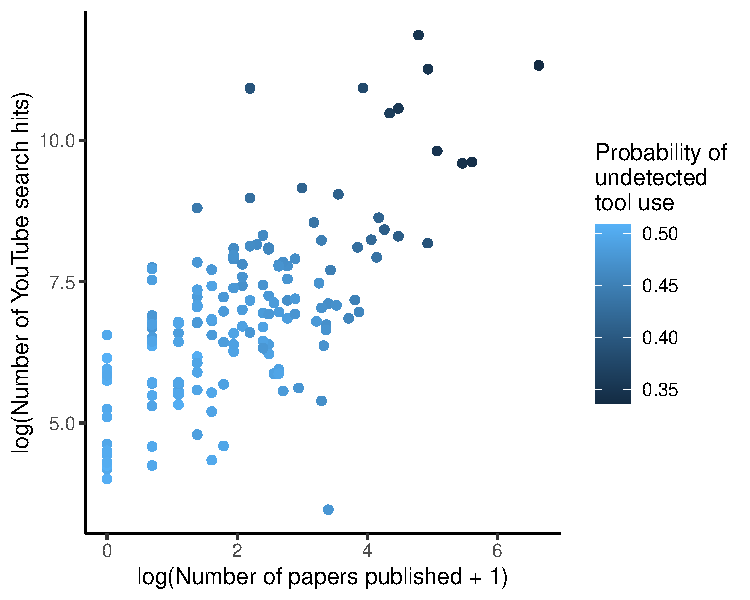
\includegraphics{manuscript_files/figure-latex/plotSurvCure3-1.pdf}
\caption{\label{fig:plotSurvCure3}\emph{Median posterior probabilities of undetected tool use for each parrot species without observed evidence of tool use from reduced model.} This reduced version of the phylogenetic survival cure model does not contain relative brain size or feeding strategy as predictors, nor does it contain any phylogenetic covariance. The only information included in the model is the number of papers published and the number of YouTube search hits for each species. Each point is a parrot species without observed evidence of tool use, and the colour of the points scales with the probability of undetected tool use. All else being equal, those species with fewer published papers and fewer YouTube search hits have a higher probability of being undetected tool users.}
\end{figure}

\newpage



\begin{figure}
\centering
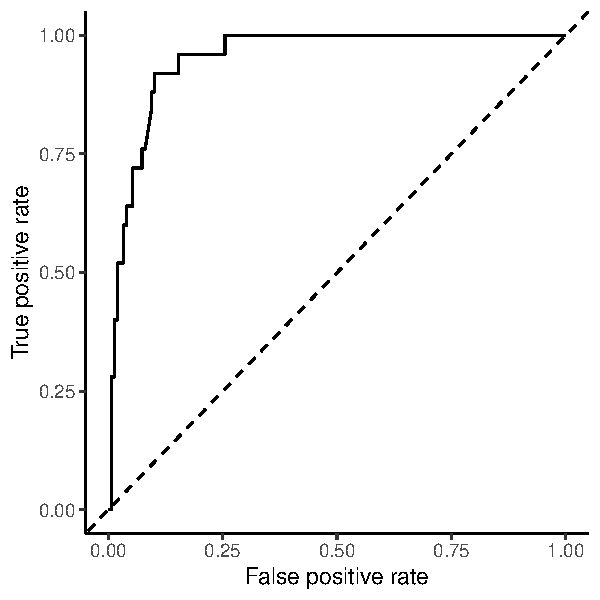
\includegraphics{manuscript_files/figure-latex/plotSurvCure9-1.pdf}
\caption{\label{fig:plotSurvCure9}\emph{Receiver operating characteristic (ROC) curve for the phylogenetic survival cure model.} The area-under-the-curve in this plot is 0.95, suggesting that the model is able to adequately classify observed tool users and non-tool users.}
\end{figure}

\newpage



\begin{figure}
\centering
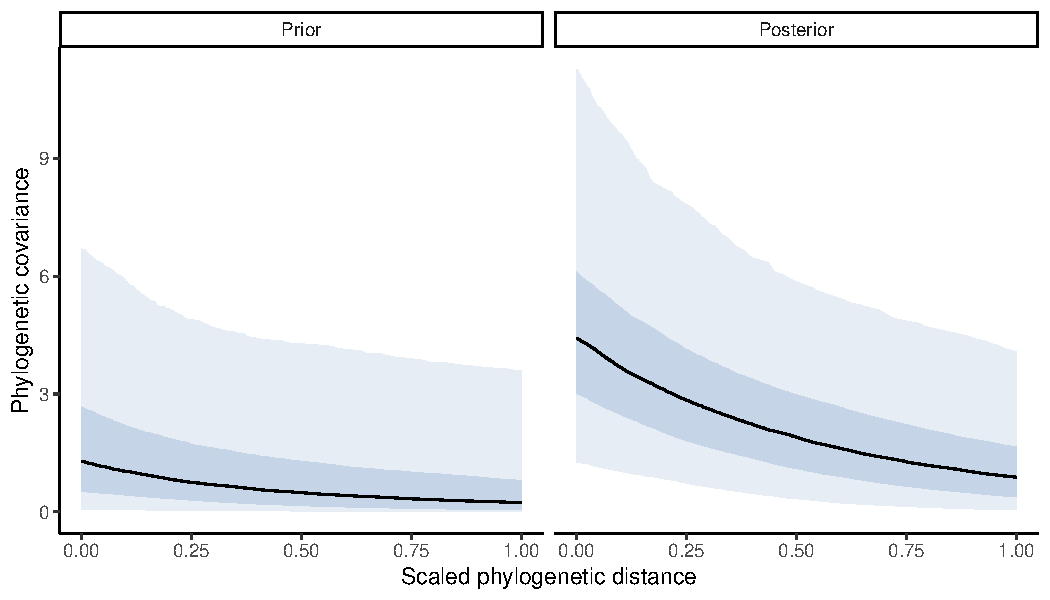
\includegraphics{manuscript_files/figure-latex/plotSurvCure5-1.pdf}
\caption{\label{fig:plotSurvCure5}\emph{Prior and posterior phylogenetic covariance functions from the Bayesian survival cure model fitted to the full dataset.} Lines are median posterior functions and shaded areas are 50\% and 95\% credible intervals.}
\end{figure}

\newpage



\begin{figure}
\centering
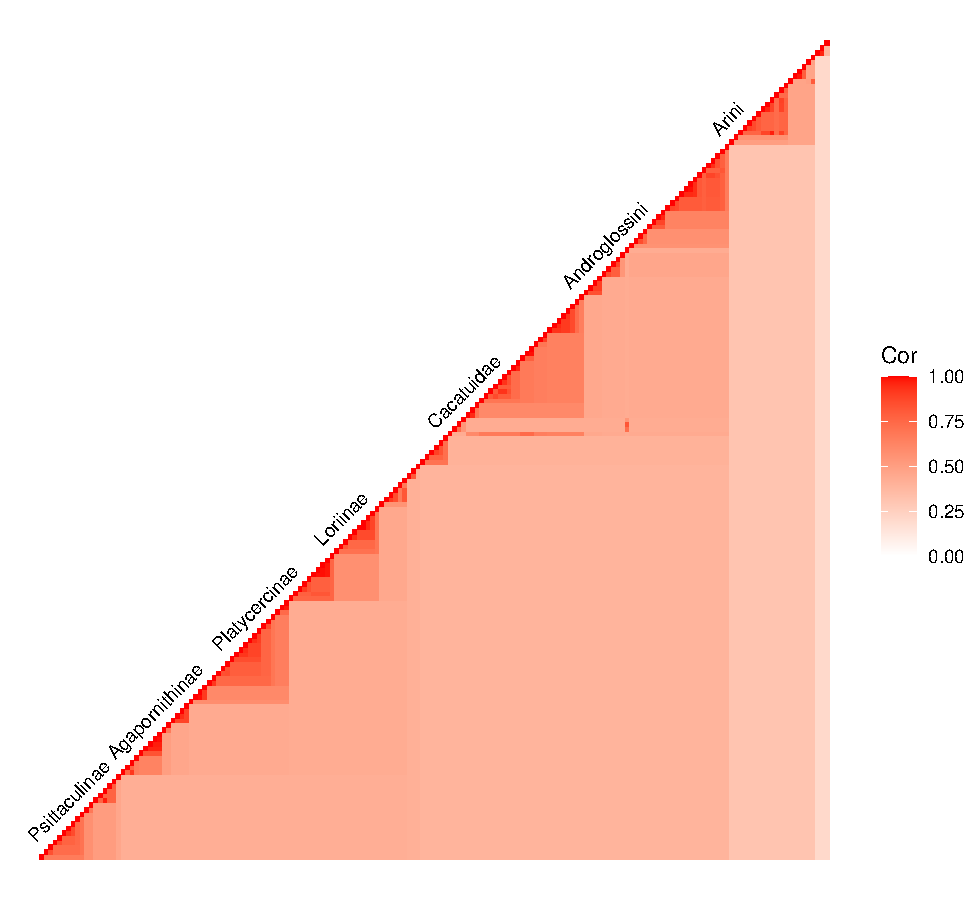
\includegraphics{manuscript_files/figure-latex/plotSurvCure6-1.pdf}
\caption{\label{fig:plotSurvCure6}\emph{Between-species correlation matrix implied by the posterior phylogenetic covariance function from the Bayesian survival cure model.} Correlations are median posterior estimates. Individual species names omitted for space reasons.}
\end{figure}

\newpage



\begin{figure}
\centering
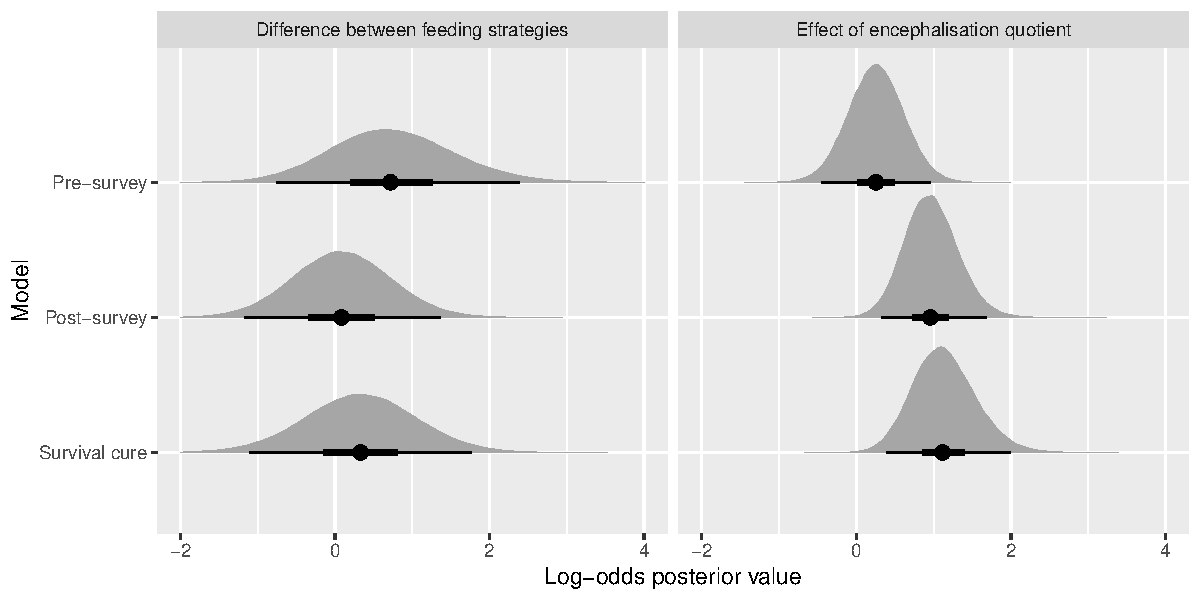
\includegraphics{manuscript_files/figure-latex/plotComparison-1.pdf}
\caption{\label{fig:plotComparison}\emph{Comparing results between the survival cure model and models fitted to the pre-survey and post-survey data without any survival cure component.} Densities are full posterior distributions from three separate models iterated over 100 posterior parrot phylogenies. Points represent posterior medians, and lines represent 50\% and 95\% credible intervals.}
\end{figure}

\newpage



\begin{figure}
\centering
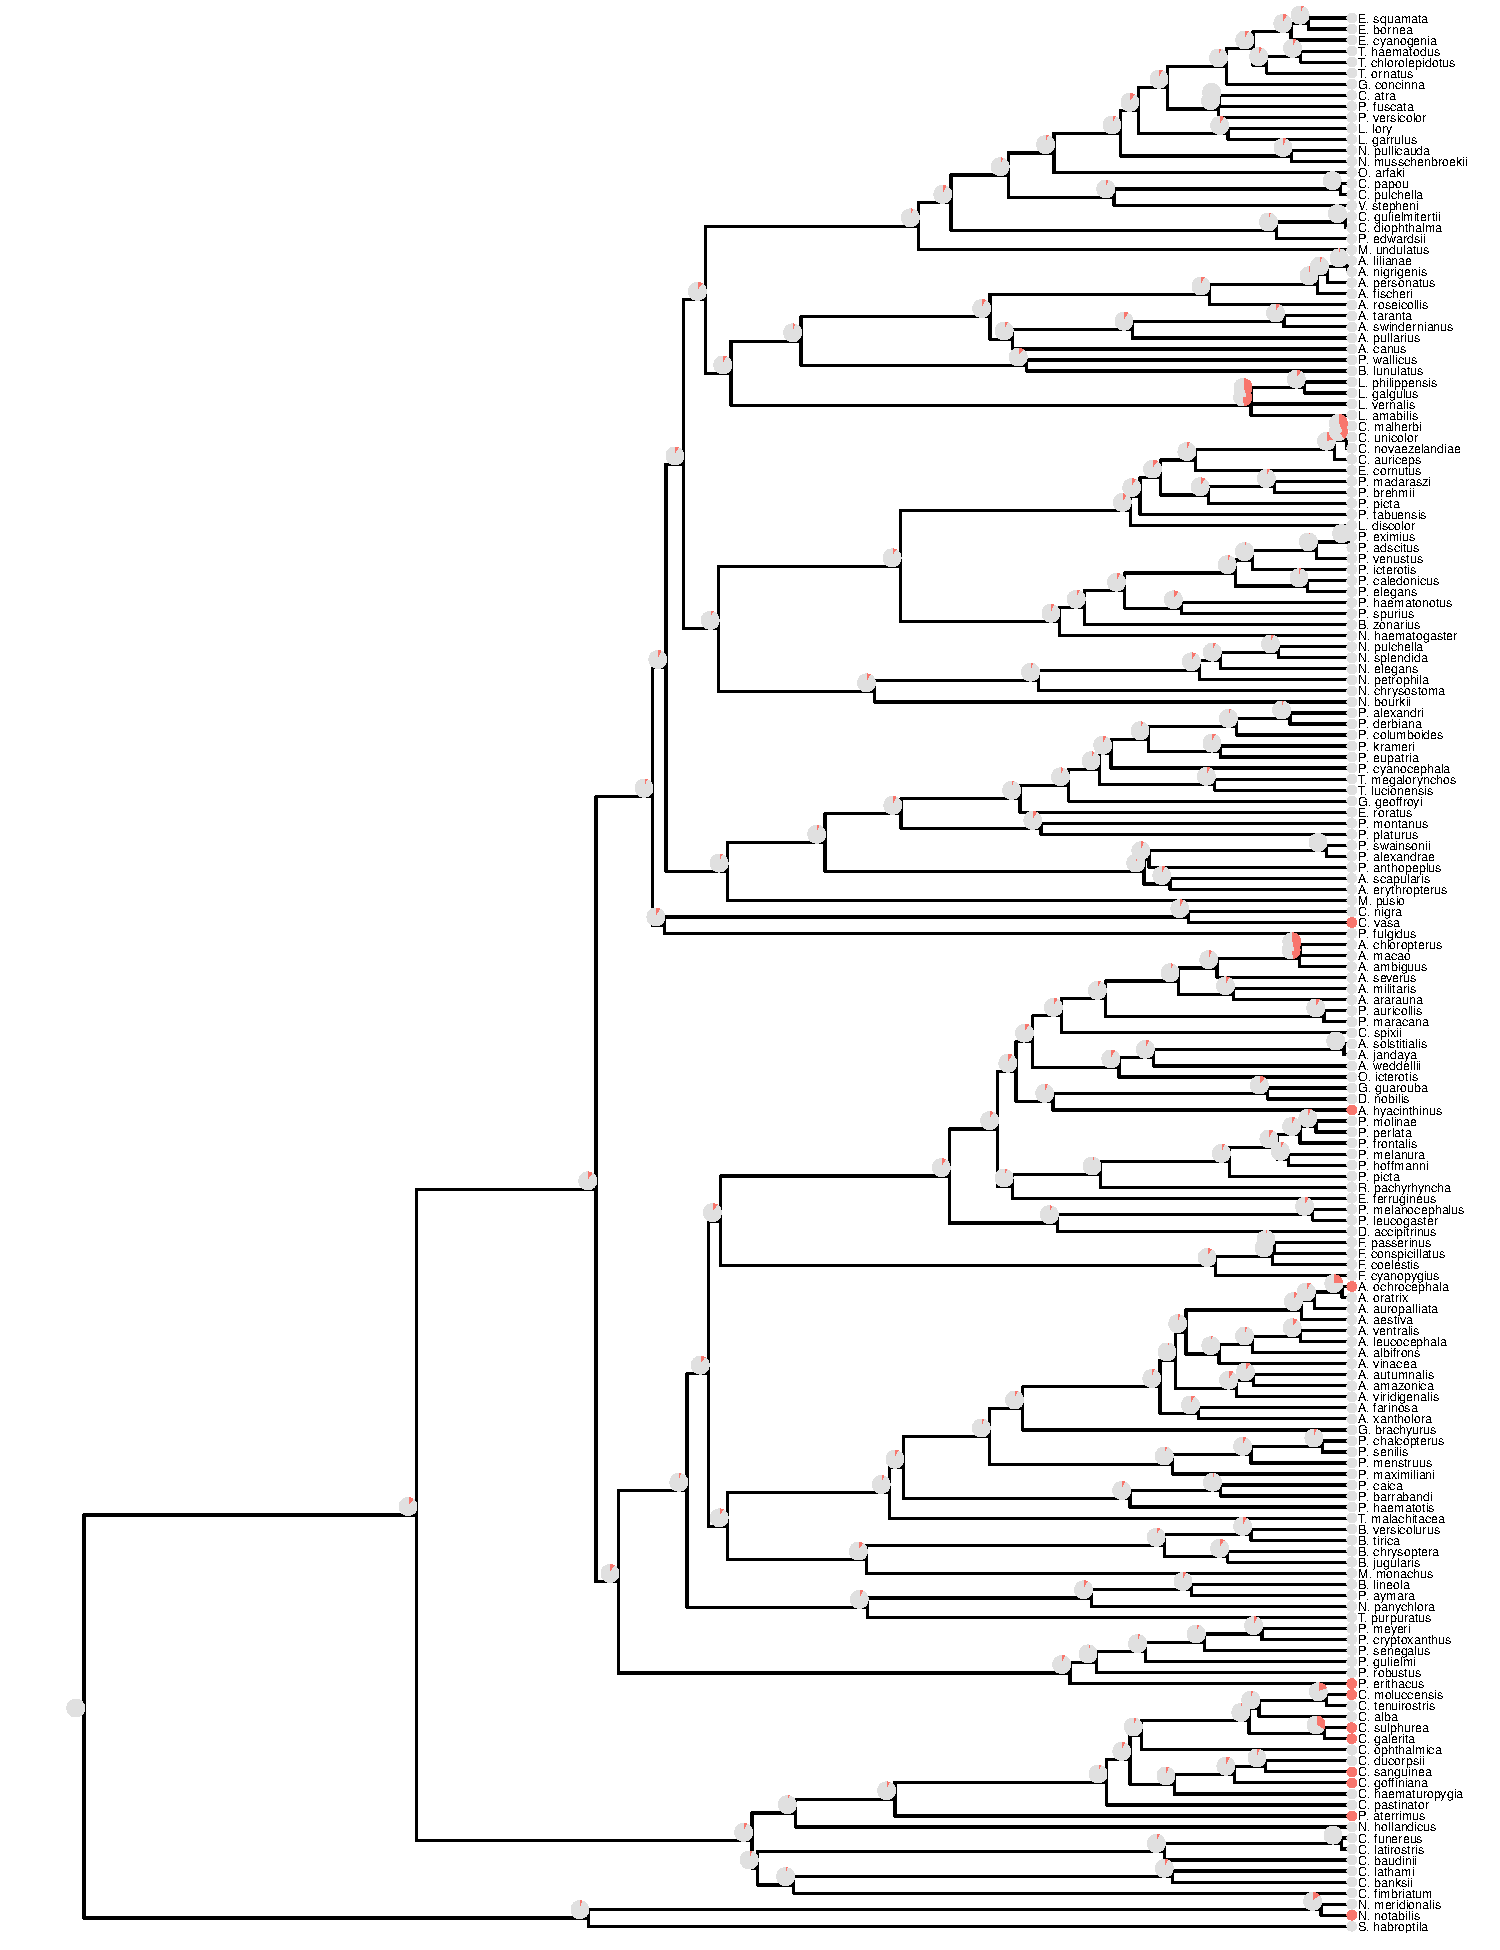
\includegraphics{manuscript_files/figure-latex/plotASR1-1.pdf}
\caption{\label{fig:plotASR1}\emph{Results of exploratory ancestral state reconstruction analysis fitted to pre-video-survey data, represented on a maximum clade credibility tree.} Tip nodes represent the presence (red) or absence (grey) of observed tool use in the scientific literature. Pie charts represent the posterior probability of tool use presence at each ancestral node.}
\end{figure}

\newpage



\begin{figure}
\centering
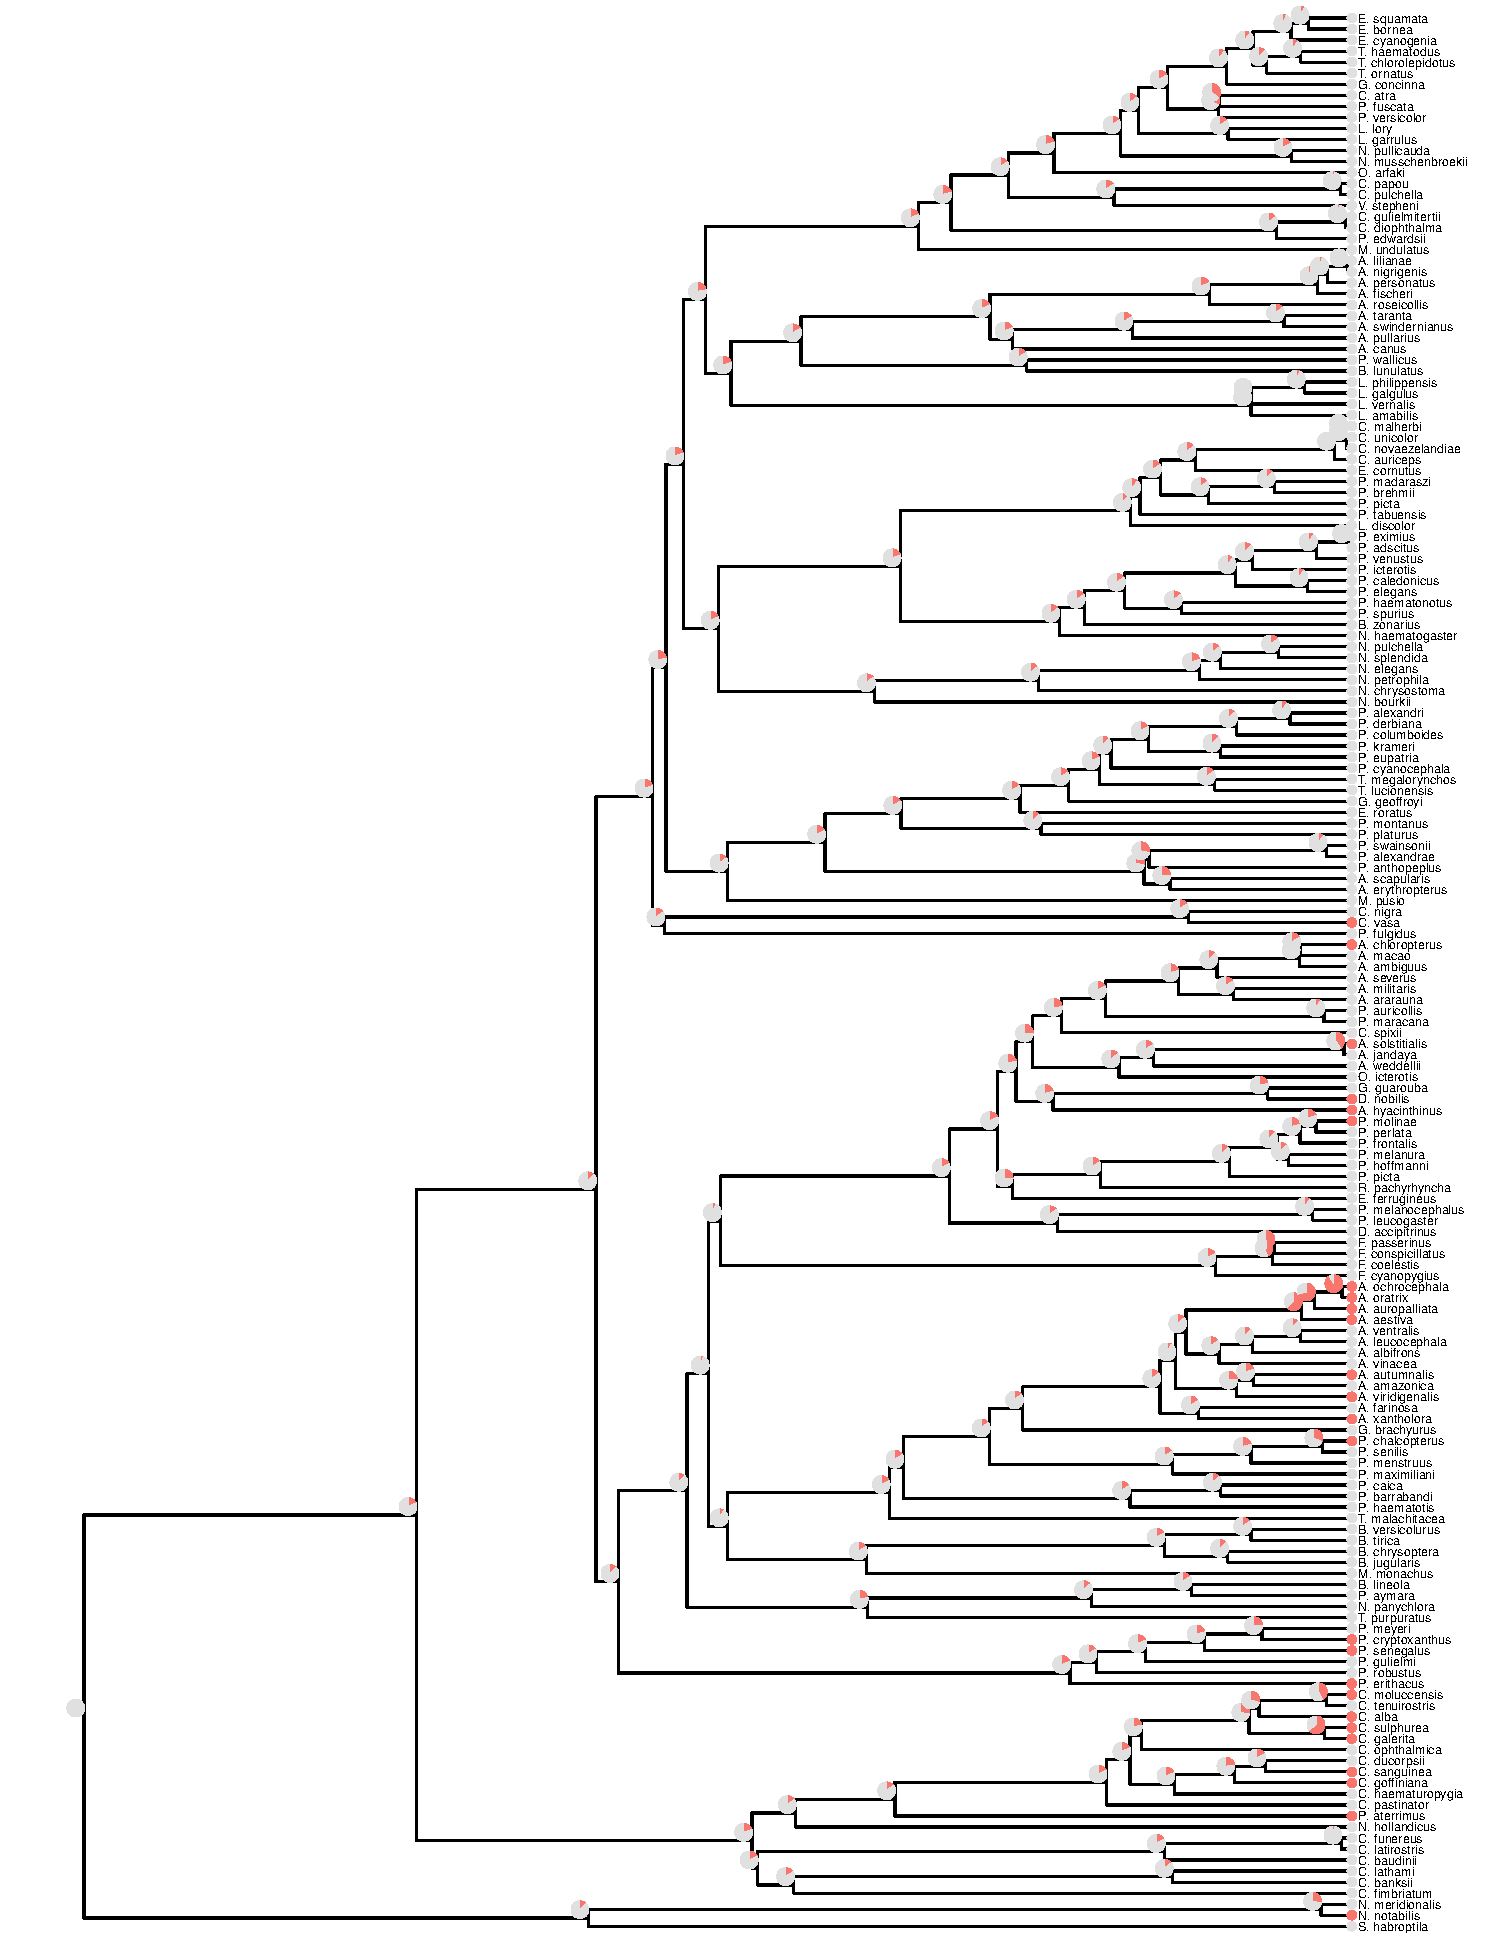
\includegraphics{manuscript_files/figure-latex/plotASR2-1.pdf}
\caption{\label{fig:plotASR2}\emph{Results of exploratory ancestral state reconstruction analysis fitted to post-video-survey data, represented on a maximum clade credibility tree.} Tip nodes represent the presence (red) or absence (grey) of observed tool use in the scientific literature and the video survey. Pie charts represent the posterior probability of tool use presence at each ancestral node.}
\end{figure}

\newpage



\begin{figure}
\centering
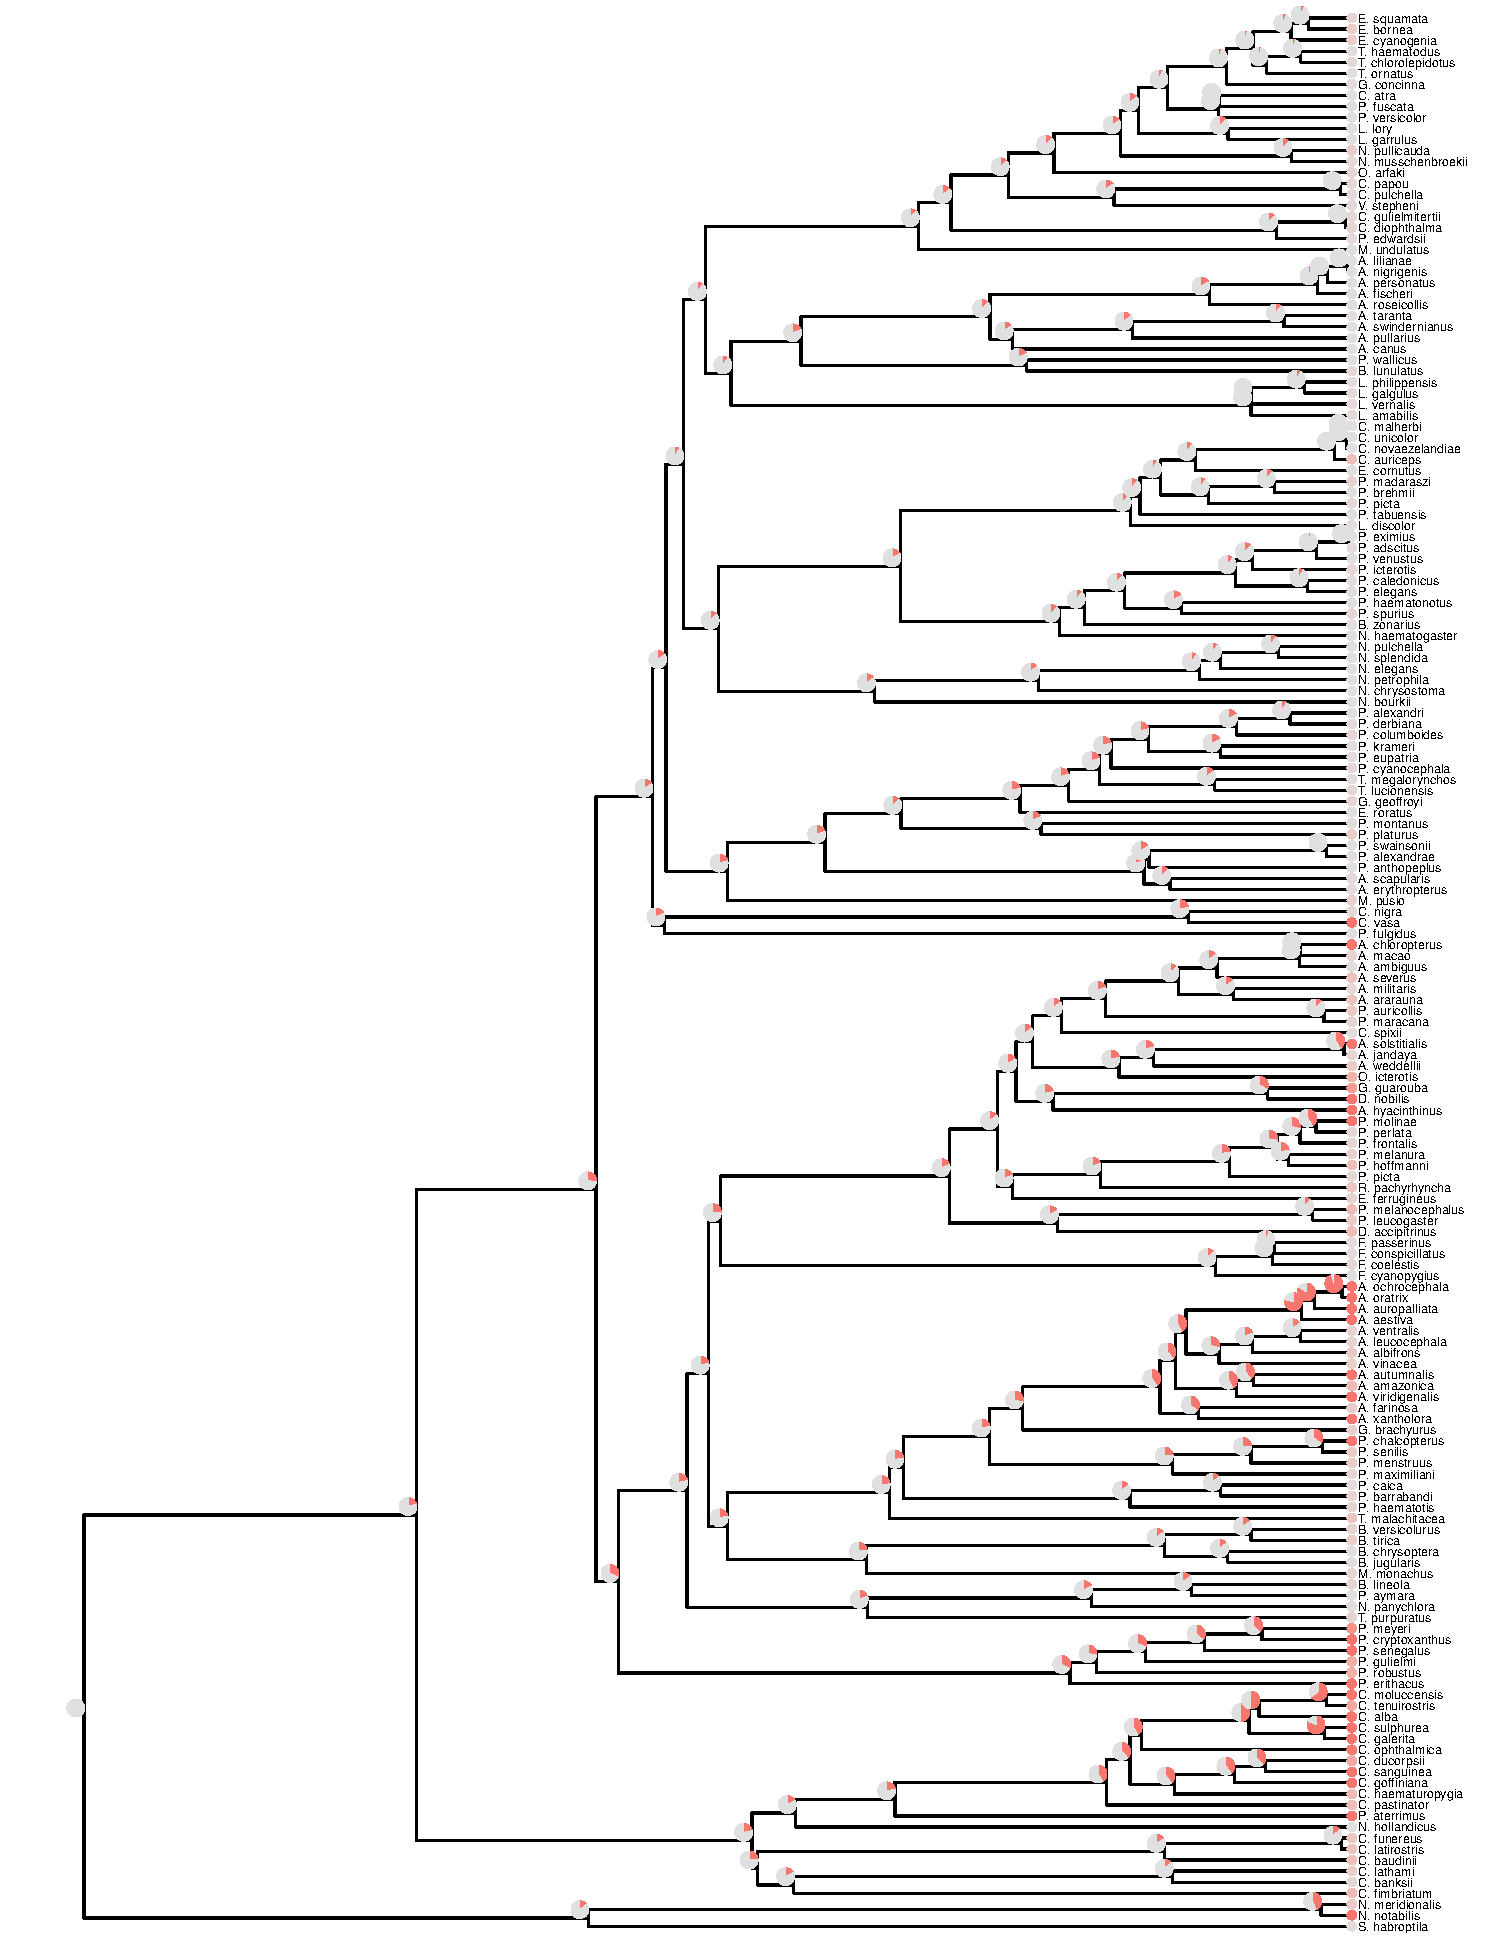
\includegraphics{manuscript_files/figure-latex/plotASR3-1.pdf}
\caption{\label{fig:plotASR3}\emph{Results of exploratory ancestral state reconstruction analysis fitted to predicted probabilities from the phylogenetic survival cure model, represented on a maximum clade credibility tree.} Tip nodes represent the median posterior predicted probabilities of tool use from the phylogenetic survival cure model, with more red indicating an increasing probability of tool use presence and more grey indicating a decreasing probability of tool use presence. Pie charts represent the posterior probability of tool use presence at each ancestral node.}
\end{figure}

\newpage



\begin{figure}
\centering
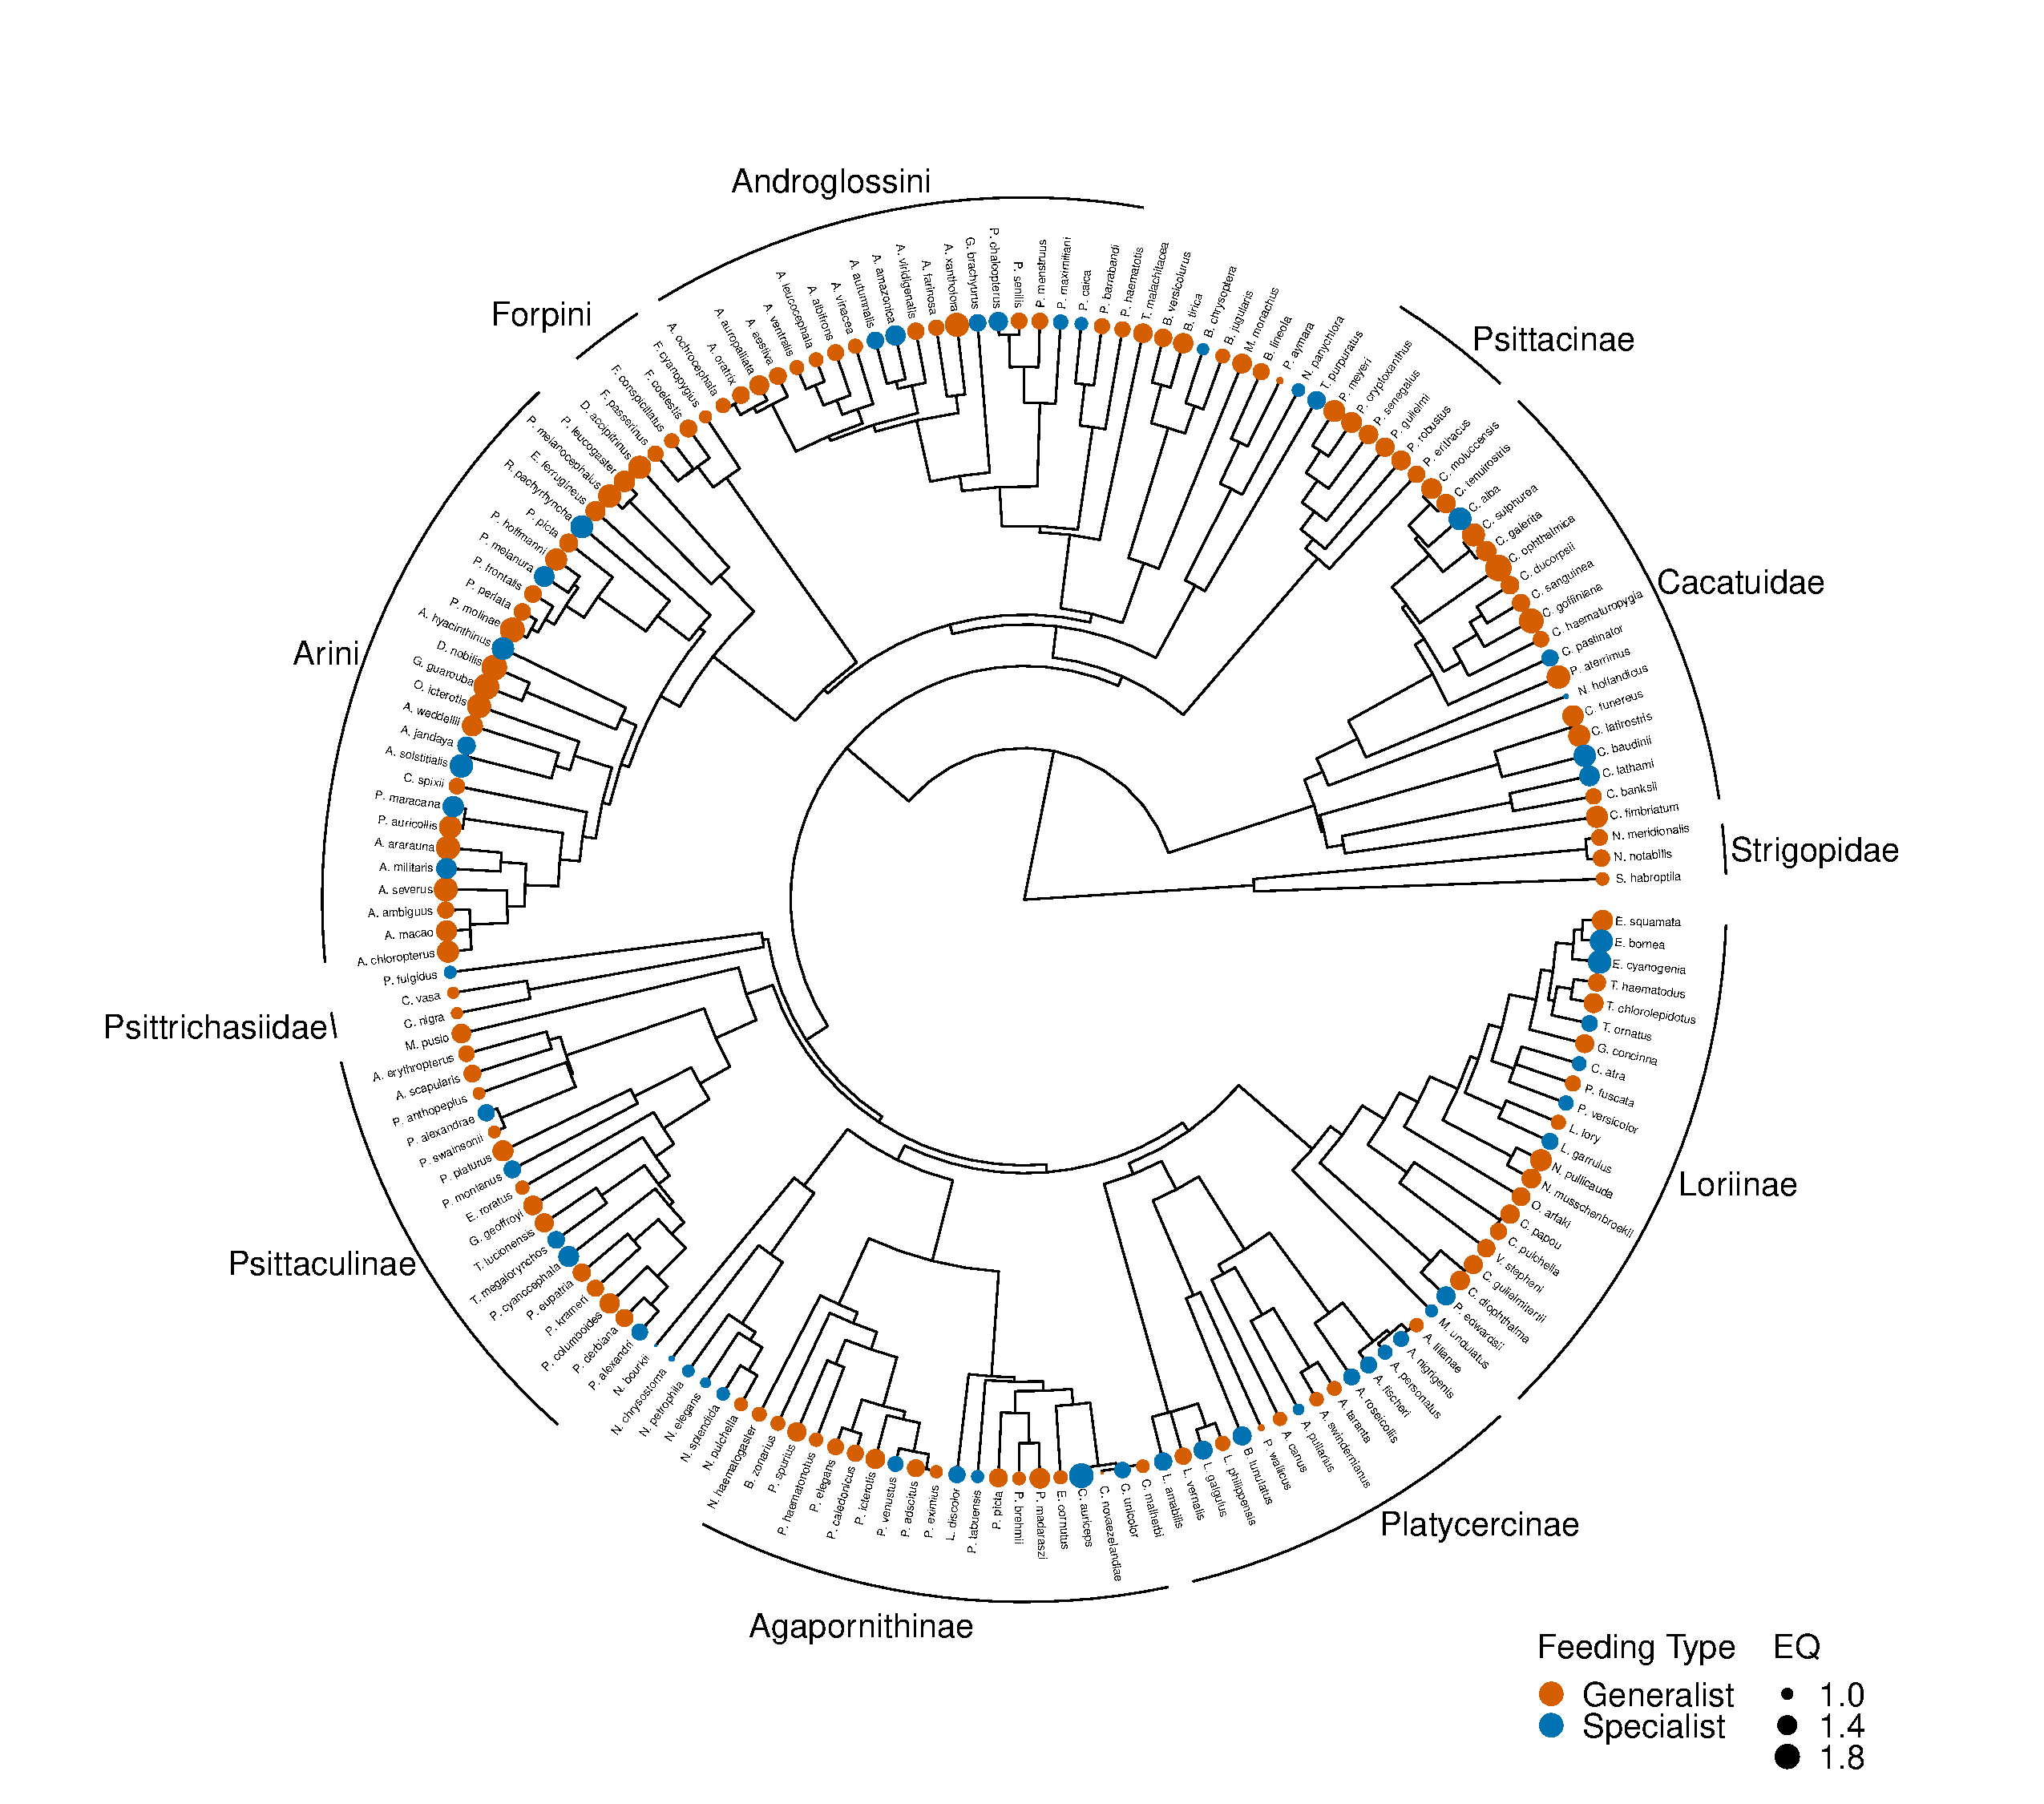
\includegraphics{manuscript_files/figure-latex/plotPhylo2-1.pdf}
\caption{\label{fig:plotPhylo2}\emph{Data on encephalisation quotient and feeding strategy for all parrots, presented on a maximum clade credibility tree.} Tip points are coloured according to feeding generalism (orange) and specialism (blue), and scaled according to encephalisation quotient (EQ).}
\end{figure}

\newpage



\begin{figure}
\centering
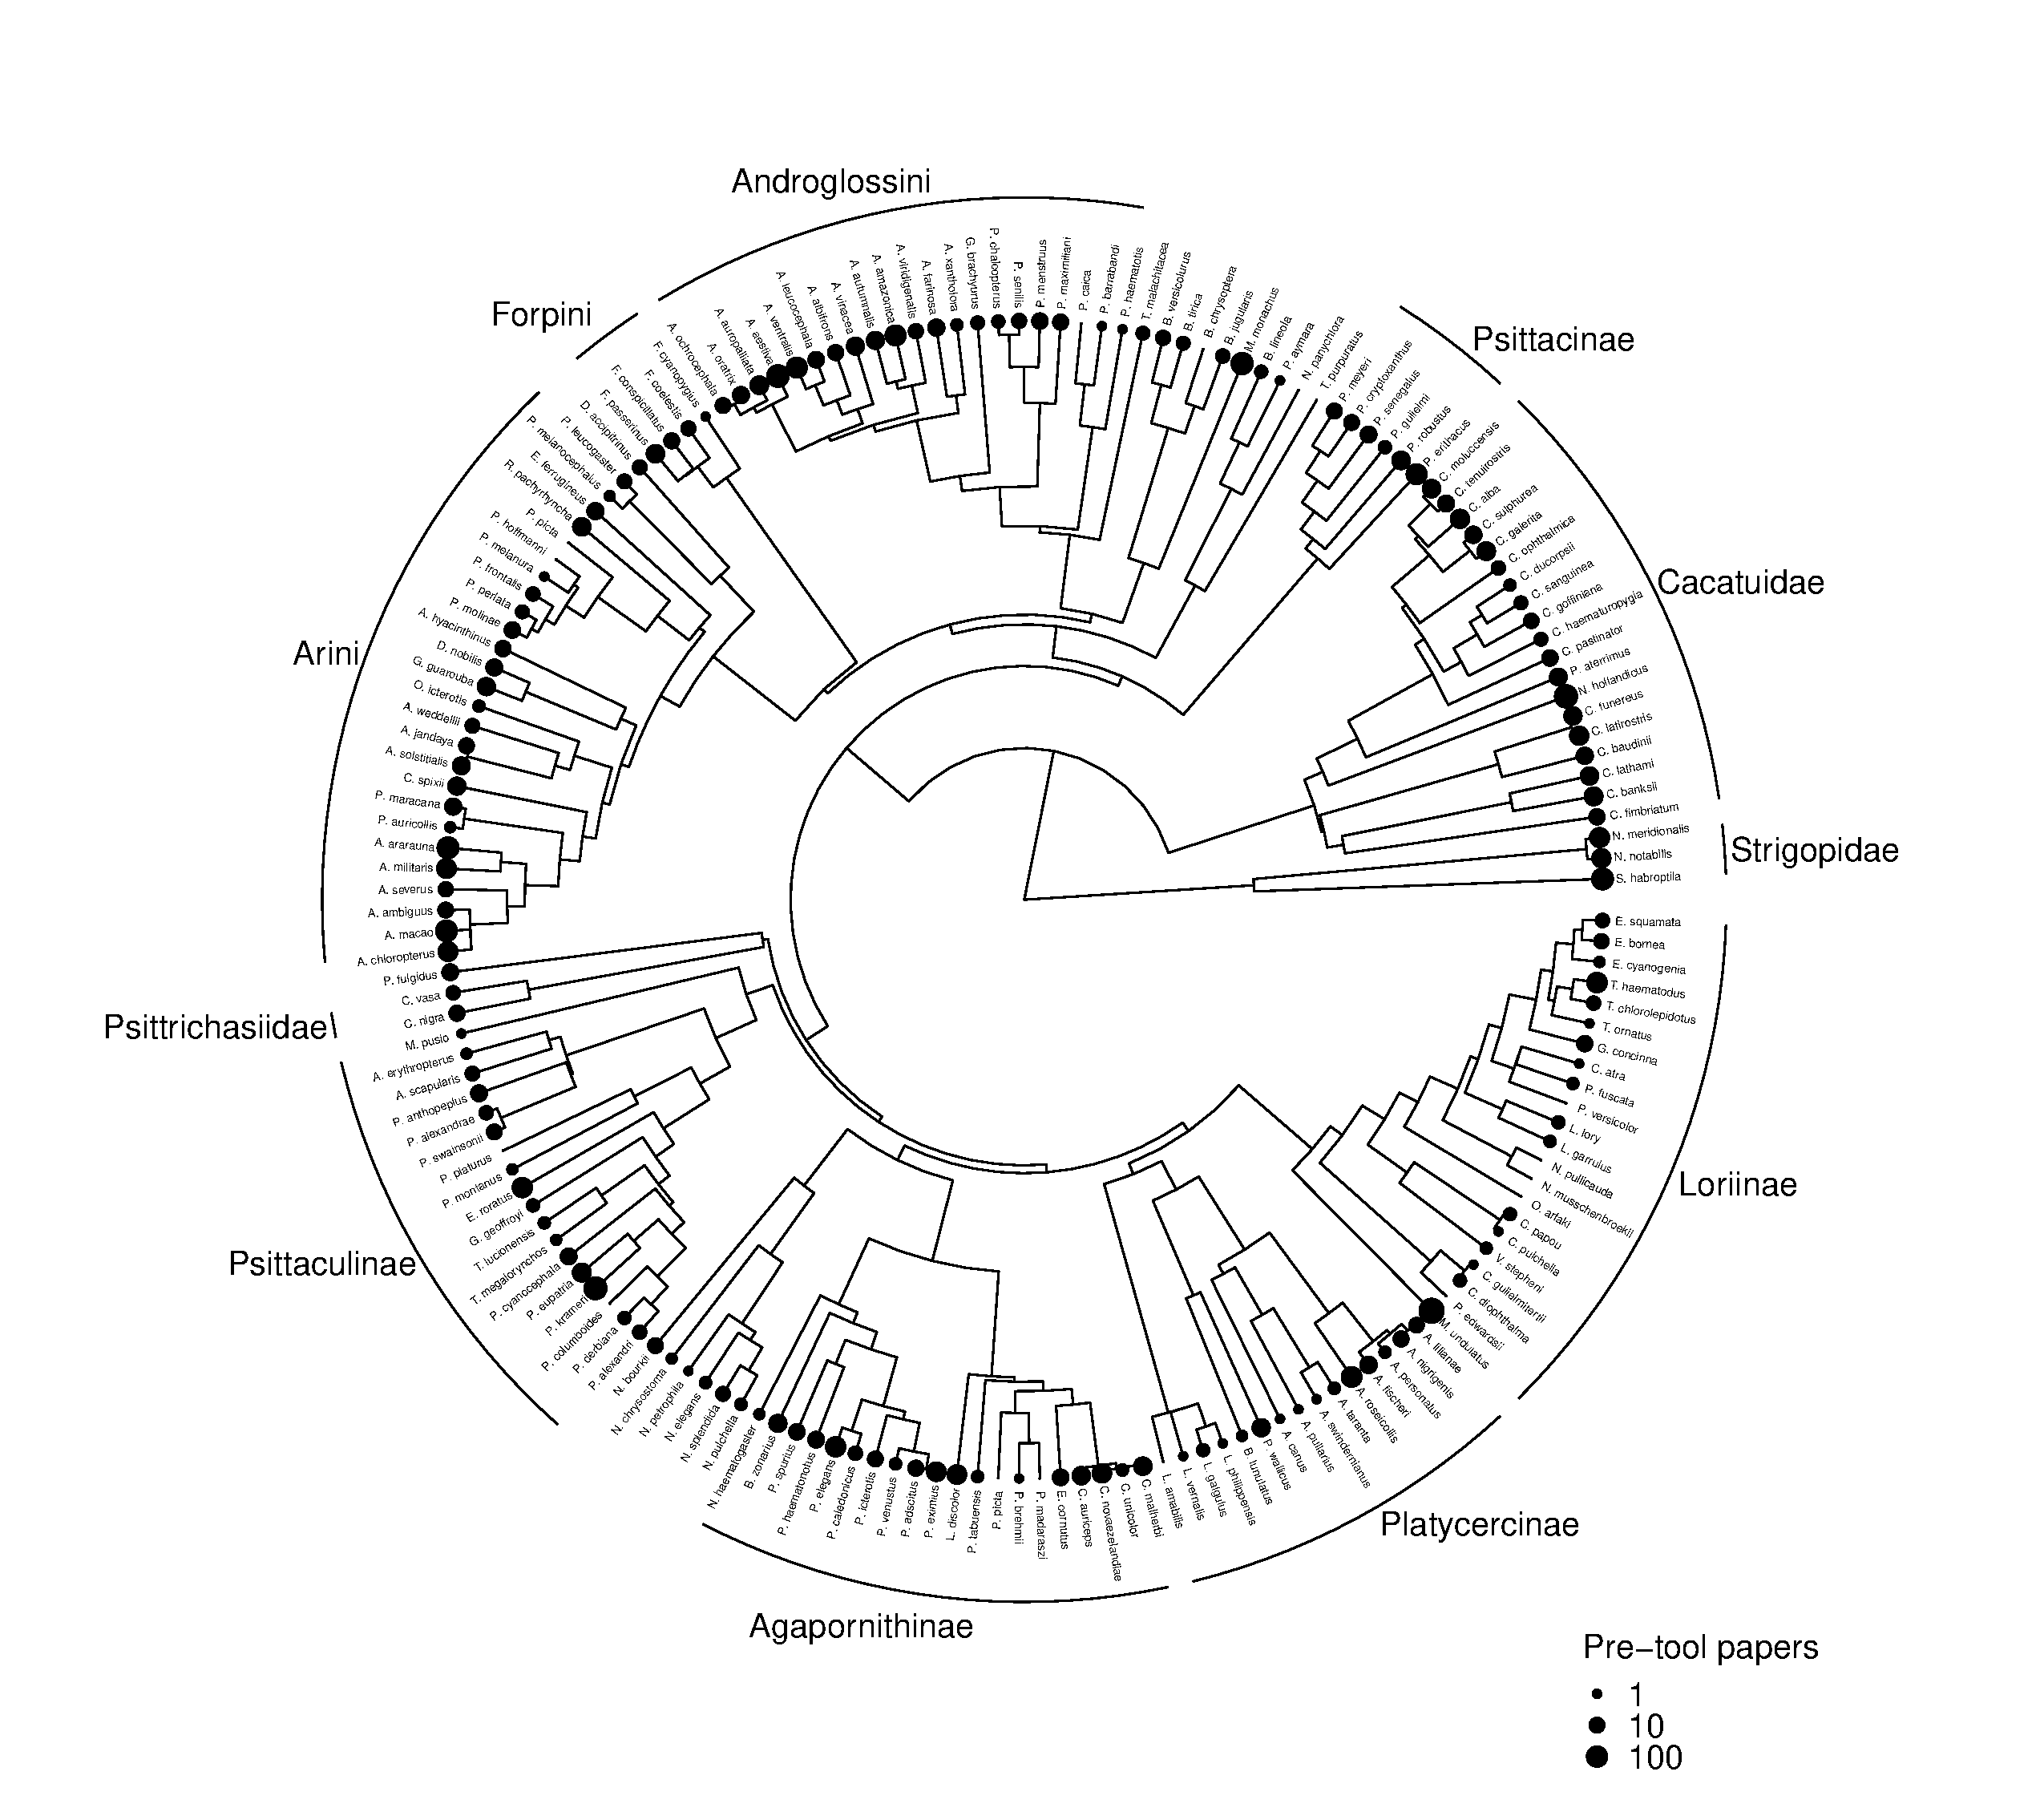
\includegraphics{manuscript_files/figure-latex/plotPhylo3-1.pdf}
\caption{\label{fig:plotPhylo3}\emph{Data on number of scientific publications until tool use discovery for all parrots, presented on a maximum clade credibility tree.} Tip points are scaled according to the number of published papers up until tool use discovery (or, if tool use has not been observed, the current number of published papers).}
\end{figure}

\newpage



\begin{figure}
\centering
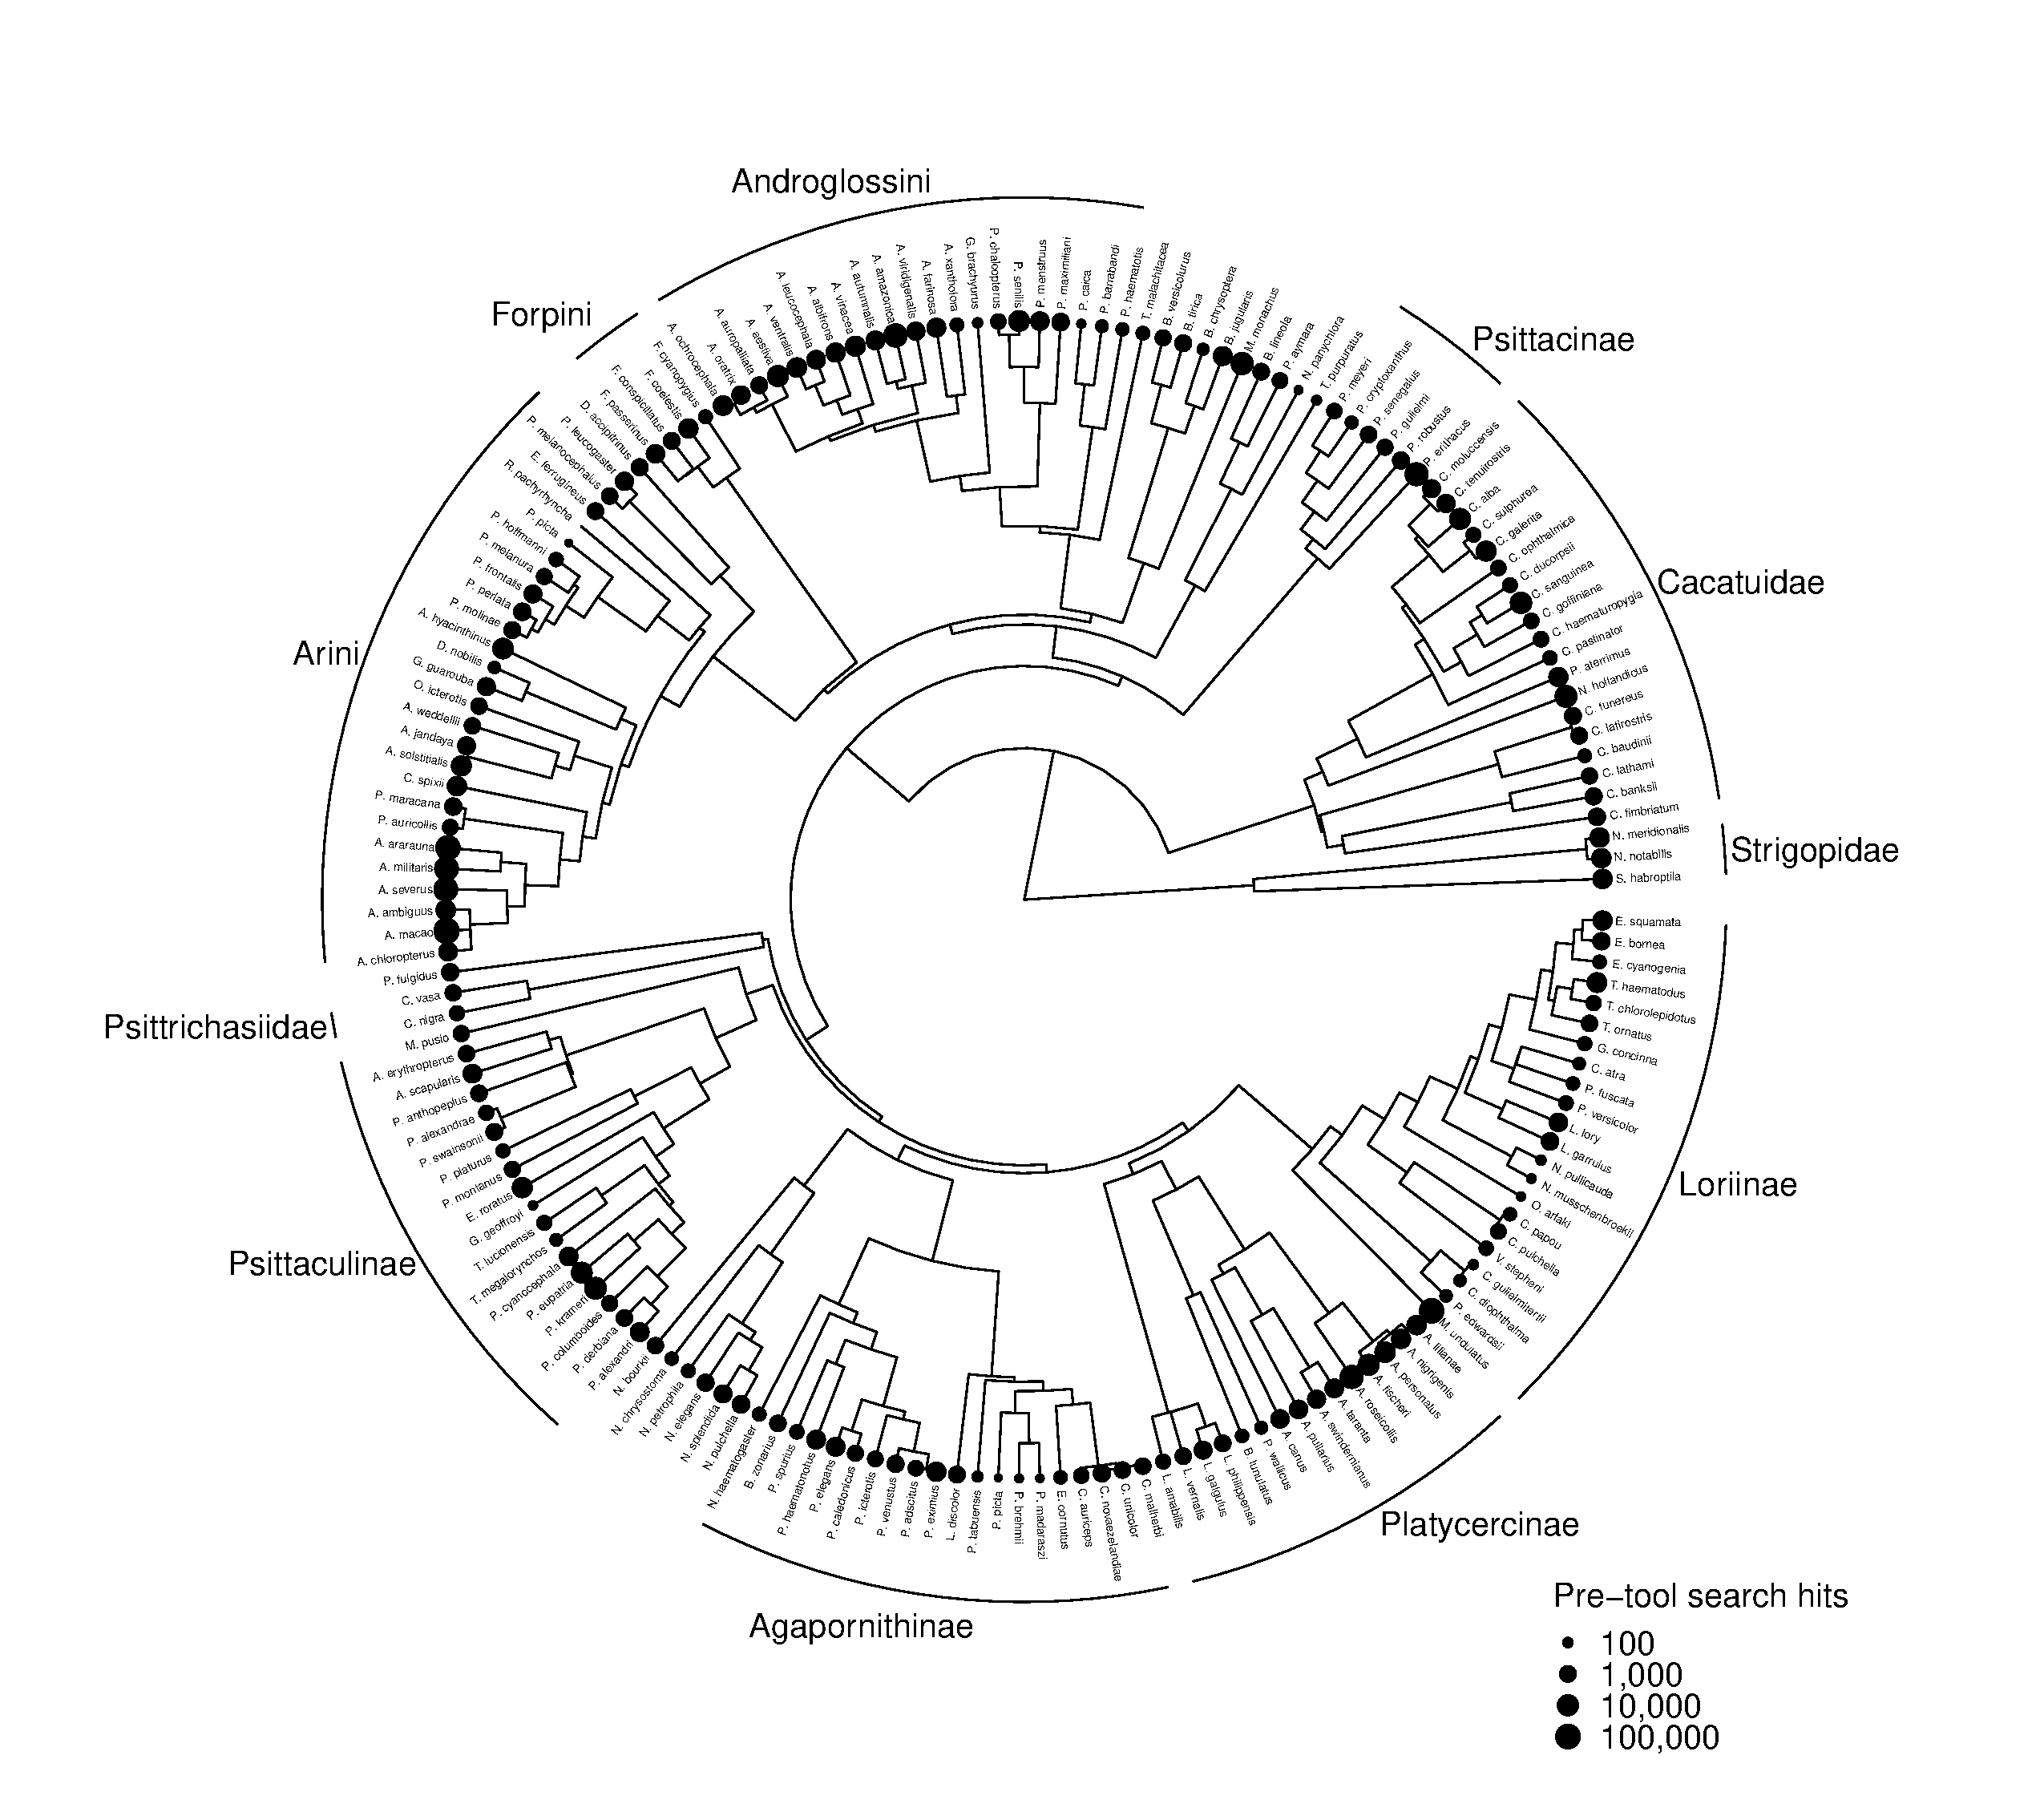
\includegraphics{manuscript_files/figure-latex/plotPhylo4-1.pdf}
\caption{\label{fig:plotPhylo4}\emph{Data on number of video search hits until tool use discovery for all parrots, presented on a maximum clade credibility tree.} Tip points are scaled according to the estimated number of video search hits up until tool use discovery (or, if tool use has not been observed, the current number of video search hits).}
\end{figure}

\newpage



\begin{figure}
\centering
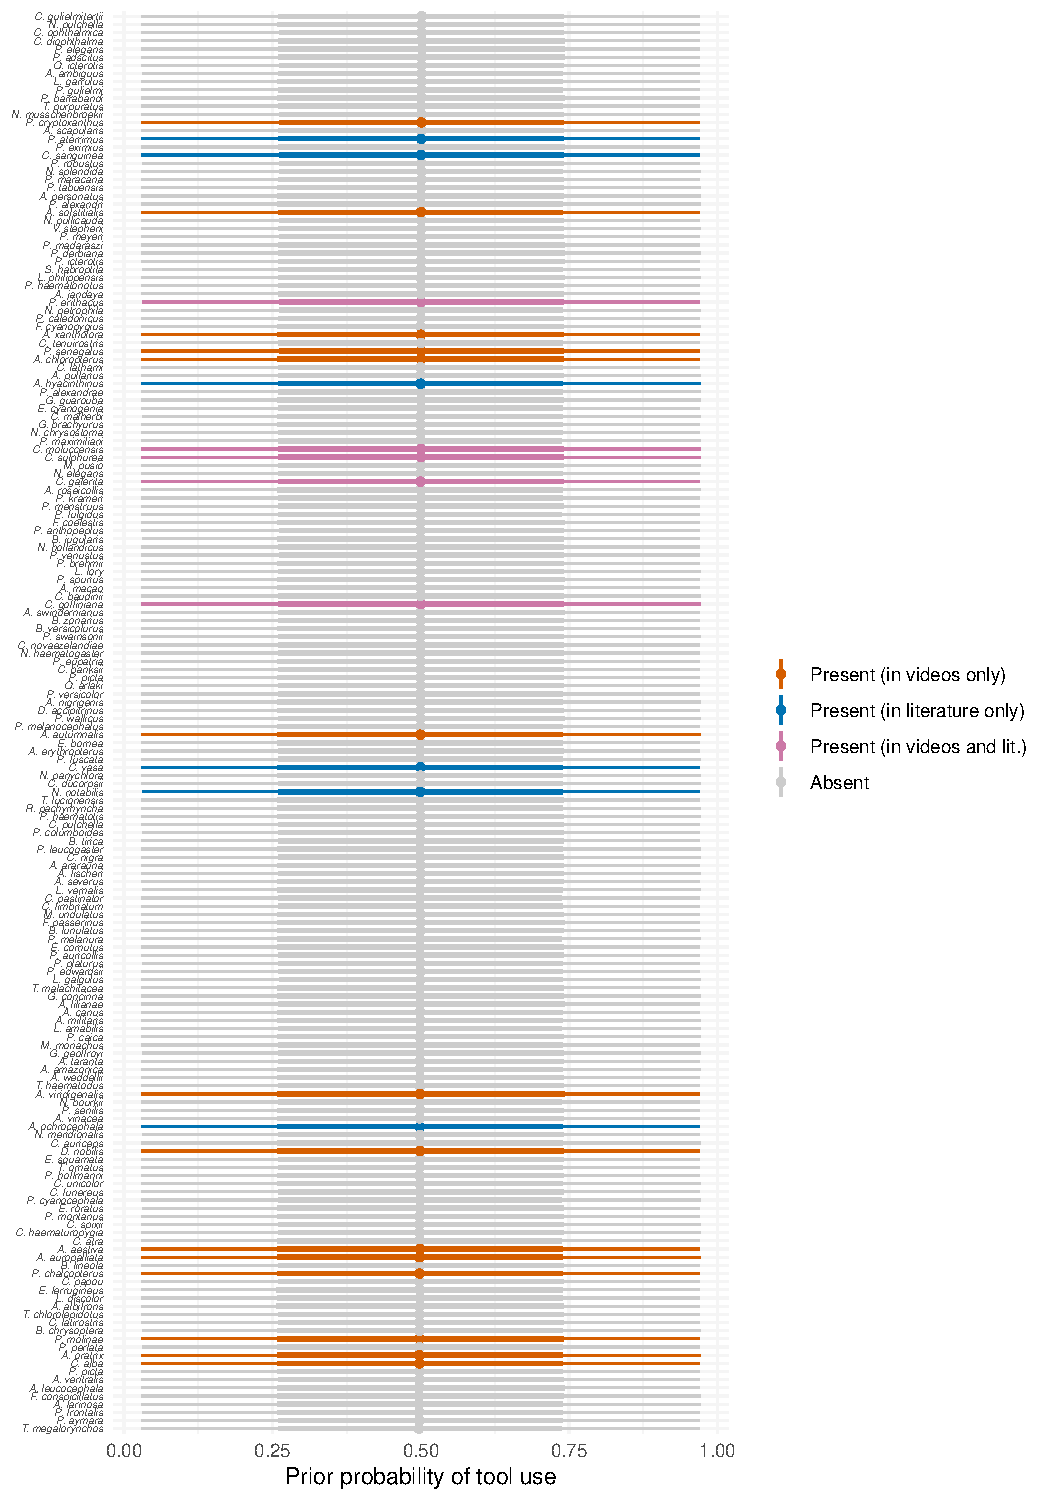
\includegraphics{manuscript_files/figure-latex/plotSurvCure7-1.pdf}
\caption{\label{fig:plotSurvCure7}\emph{Prior predicted probabilities of tool use for each species from our phylogenetic survival cure model.} Points are prior medians and lines are 50\% and 95\% credible intervals.}
\end{figure}

\newpage



\begin{figure}
\centering
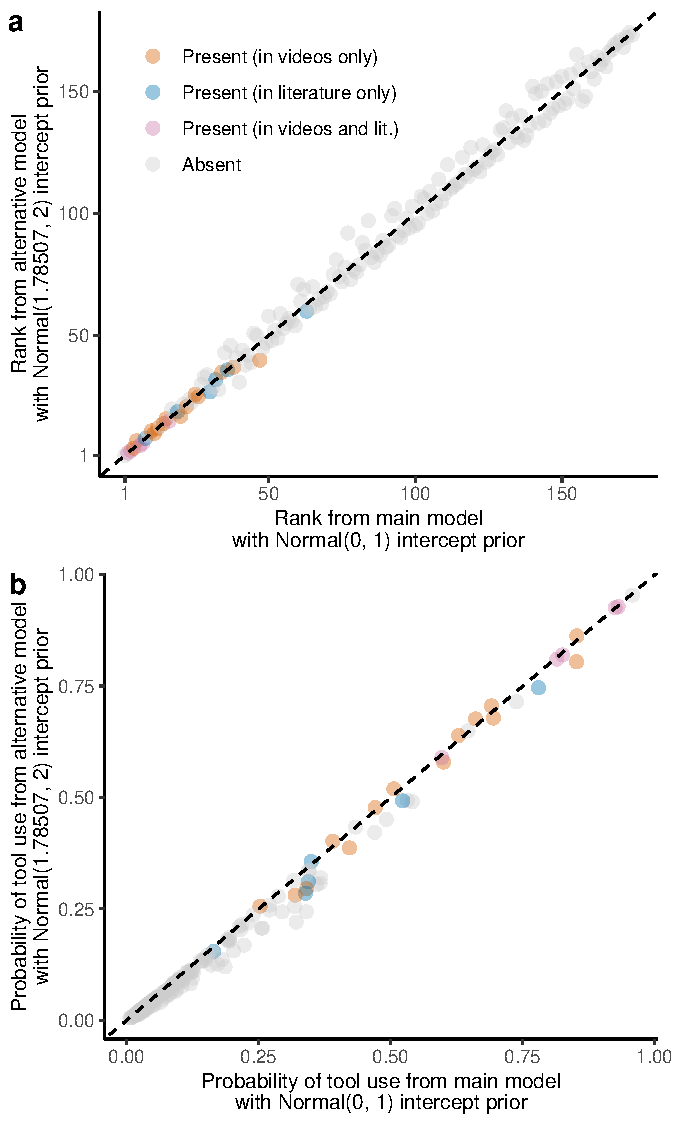
\includegraphics{manuscript_files/figure-latex/plotSurvCure8-1.pdf}
\caption{\label{fig:plotSurvCure8}\emph{Results of sensitivity analysis.} The phylogenetic survival cure model was fitted with either a standard Normal(0, 1) prior on the intercept or an alternative Normal(1.78507, 2) prior on the intercept. This latter prior is wider on the logit scale and roughly converts to a 0.86 prior probability of non-tool-use (or a 0.14 prior probability of tool-use, which is the proportion of tool users in the dataset). The sensitivity analysis showed that changing this intercept prior did not have a marked impact on (a) the posterior rankings of parrot species from 1st to 174th or (b) the median posterior probabilities of tool use for parrot species.}
\end{figure}

\newpage



\begin{figure}
\centering
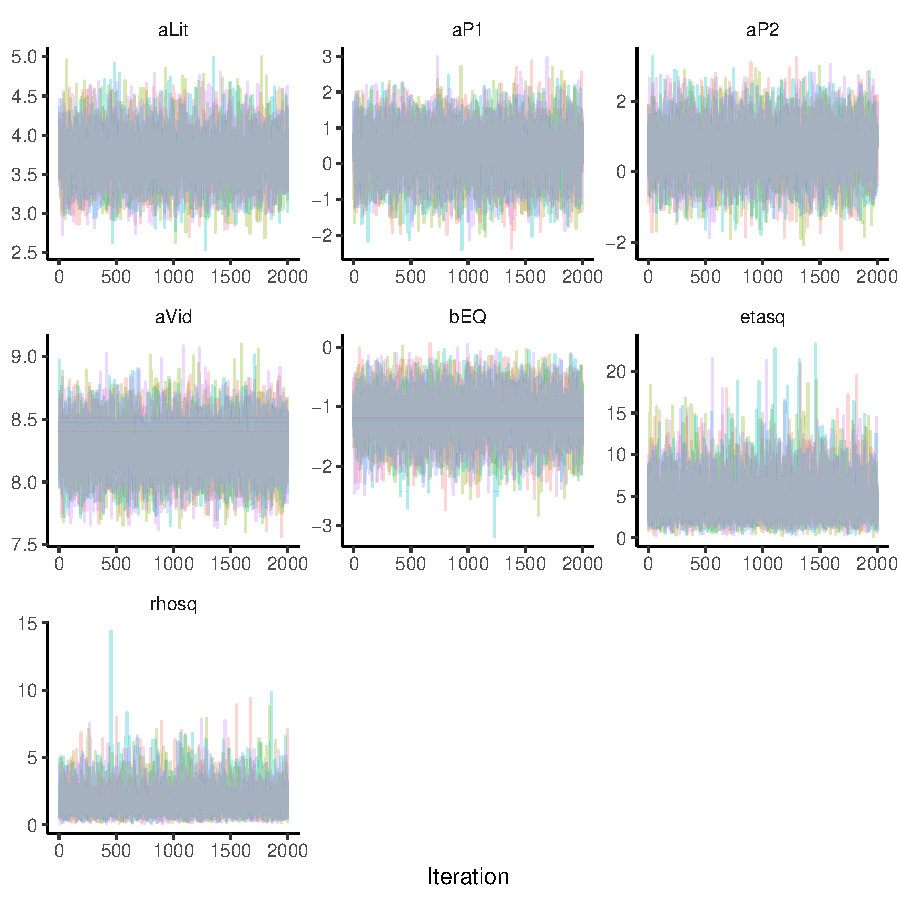
\includegraphics{manuscript_files/figure-latex/plotTrace-1.pdf}
\caption{\label{fig:plotTrace}\emph{Trace plots for the Bayesian phylogenetic survival cure model.} Only four chains are shown for ease of presentation.}
\end{figure}

\newpage



\begin{figure}
\centering
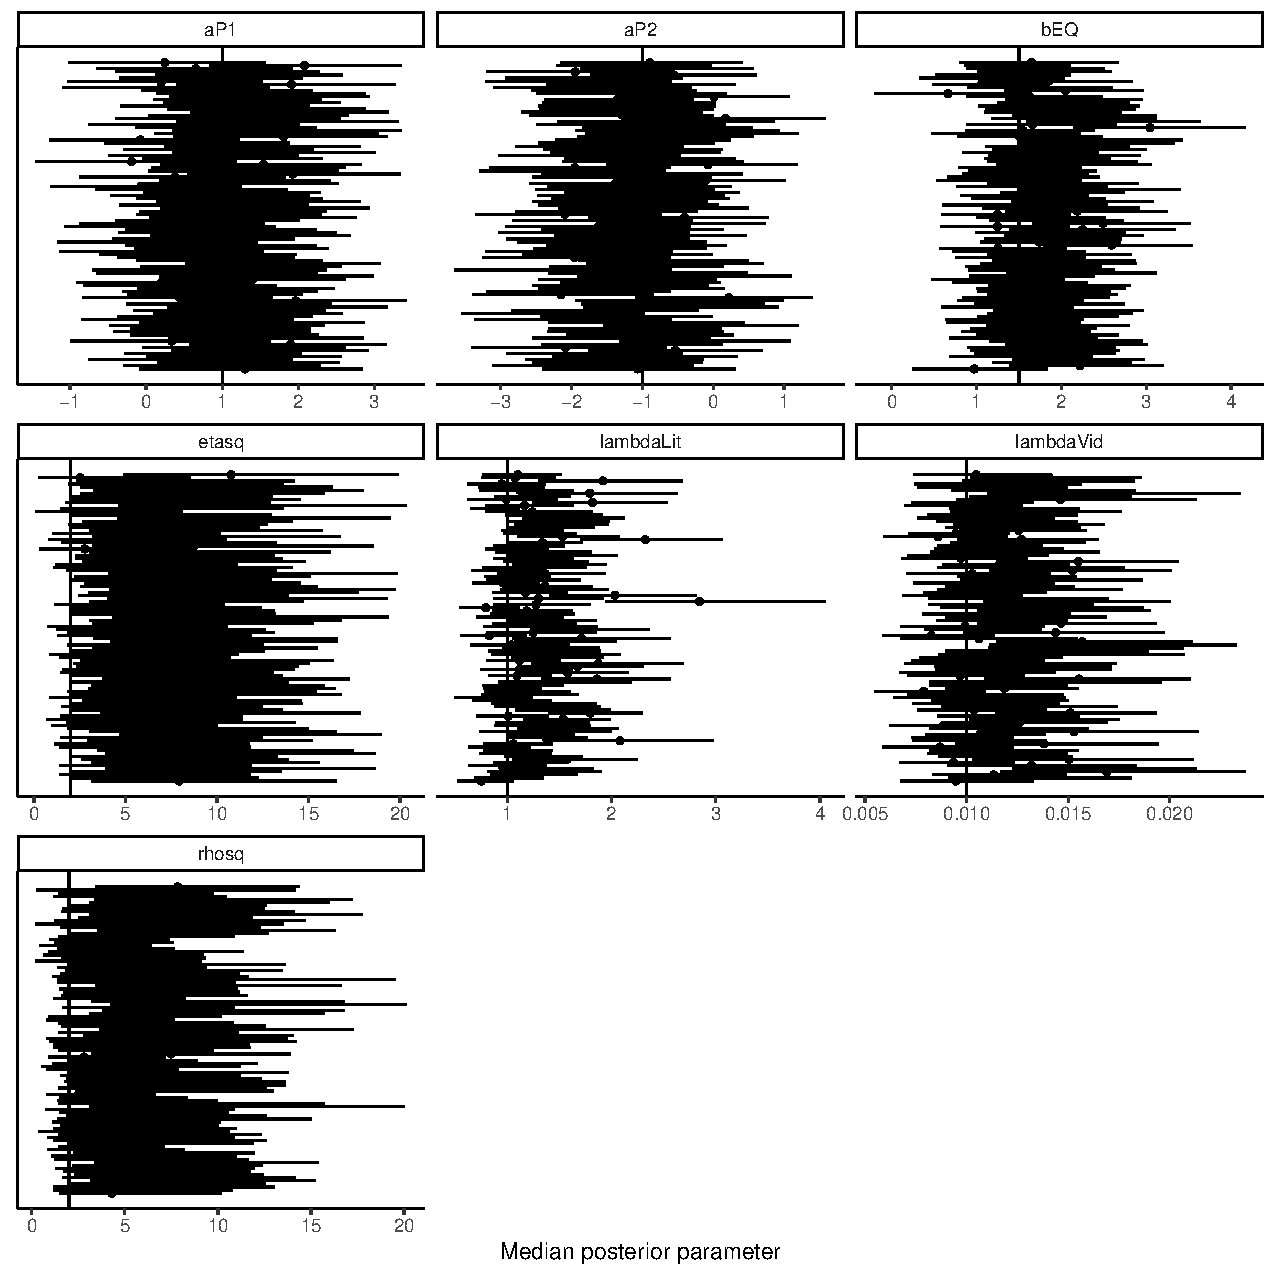
\includegraphics{manuscript_files/figure-latex/plotSurvCureSim-1.pdf}
\caption{\label{fig:plotSurvCureSim}\emph{Posterior estimates from Bayesian survival cure models fitted to 100 datasets simulated with known parameters.} Each dataset consisted of 100 species. Known parameters are presented as solid vertical lines, whereas points and horizontal lines represent posterior medians and 95\% credible intervals. The models were successfully able to recapture the parameters from the simulated datasets.}
\end{figure}


\end{document}
